\chapter{التطبيق خطوة بخطوة}
\label{ch:01b-build}

\section{ما الذي سنطبّقه؟}
\label{sec:build-start}

لنفترض أن لدينا مؤسسة اسمها «وزارة الاقتصاد والصناعة»، وتريد تنظيم الكشف على المنشآت التجارية. يكلّف أحمد الباحث نور بالكشف على «فرن الأمانة». يزور نور الفرن ويسجل نتيجة الزيارة في استمارة، ثم يرسلها إلى ريم للتدقيق. تقرأ ريم الكشف، ثم تختار واحداً من ثلاثة قرارات: تعتمده، أو تعيده إلى نور لاستكمال النواقص، أو ترفضه مع ذكر السبب. وعندما تعتمد ريم الكشف، تنتقل التصحيحات التي سجلها نور (مثل عنوان الفرن الجديد) إلى ملف الفرن تلقائياً.

سنبني هذا العمل كله من الصفر، بالترتيب الذي يحتاجه النظام: كل خطوة تعتمد على ما قبلها، فلا تقفز فوق خطوة.

\begin{table}[H]
\centering
\caption{فريق المثال}
\label{tab:team}
\begin{tabularx}{\linewidth}{R{4cm} R{4cm} Y}
\rcHeaderRow
\thh{الشخص} & \thh{منصبه} & \thh{عمله في العملية}\\
أحمد سالم — تجريبي & رئيس فريق الكشف الميداني — 01 & يجهّز التكليف ويتابع النتائج في لوحة المؤشرات.\\
نور حسن — تجريبي & باحث ميداني — 01 & يزور المنشأة ويعبئ استمارة الكشف ويرسلها.\\
ريم خالد — تجريبي & مدقق كشوف المنشآت — 01 & تراجع الكشف وتتخذ القرار.\\
\end{tabularx}
\end{table}

\subsection{خريطة العمل من البداية إلى النهاية}

\begin{enumerate}
\item \textbf{الفريق:} نُنشئ مكان الفريق في الهيكل، ثم الوظائف والمناصب، ثم الأشخاص، ونربط كل شخص بمنصبه.
\item \textbf{ملف المنشأة:} نُنشئ تطبيقاً يجمع عمل الفريق، ونوع سجلات اسمه «المنشآت التجارية» يحفظ بيانات كل منشأة، ثم نضيف «فرن الأمانة».
\item \textbf{استمارة الكشف:} نُنشئ نموذجاً بأسئلته وقواعده، ونربطه بملف المنشأة.
\item \textbf{الموافقة:} نحدد كيف ينتقل الكشف من نور إلى ريم، وما الذي يحدث بعد كل قرار.
\item \textbf{الوصول والنشر:} نمنح كل شخص ما يحتاجه فقط، ثم ننشر النموذج ونجربه.
\item \textbf{التكليف والتنفيذ:} يكلّف أحمد نور بالكشف، فيعبئه نور، وتقرر ريم.
\item \textbf{لوحة المؤشرات:} نعرض المنشآت في أرقام ورسوم وجدول، مع بحث وتصفية.
\end{enumerate}

\subsection{كيف تقرأ هذا الدليل؟}

\begin{itemize}
\item كل كلمة بين «» هي النص الذي تراه على الشاشة كما هو، مثل زر «إنشاء». ابحث عنها بعينك قبل الضغط.
\item السهم ← يعني «ثم افتح»: «الموارد البشرية» ← «الأعضاء» تعني: افتح تطبيق الموارد البشرية، ثم صفحة الأعضاء.
\item كل خطوة تبدأ بـ\textbf{لماذا؟}، ثم جدول بالحقول، ثم ما تضغطه وتكتبه، ثم \textbf{تحقق:} لتتأكد أن الخطوة نجحت قبل الانتقال.
\item في جداول الحقول: \req{} يعني أن النظام لا يحفظ بدون هذا الحقل، و\rec{} يعني أننا ننصح بتعبئته في هذا المثال، و\opt{} يعني أنك تستطيع تركه فارغاً، و\gen{} يعني أن النظام يملؤه وحده. أي حقل لا يذكره الجدول اتركه كما هو.
\item الحقل المطلوب الذي يبقى فارغاً تظهر تحته كلمة «مطلوب» باللون الأحمر، وتبقى الصفحة مكانها دون حفظ. هذا ليس عطلاً: أكمل الحقل ثم اضغط الزر مرة أخرى.
\end{itemize}

\begin{table}[H]
\centering
\caption{كلمات ستتكرر في الدليل}
\label{tab:glossary}
\begin{tabularx}{\linewidth}{R{3.2cm} Y}
\rcHeaderRow
\thh{الكلمة} & \thh{معناها ببساطة}\\
الوحدة التنظيمية & مديرية أو دائرة داخل المؤسسة، مثل «دائرة حماية المستهلك».\\
المنصب & كرسي وظيفي محدد في وحدة، مثل «باحث ميداني — 01». يبقى المنصب حتى لو تغيّر الشخص الذي يشغله.\\
العضو & حساب شخص في النظام، مثل نور.\\
التعيين & الرابط الذي يقول: «نور يشغل منصب الباحث». بدونه لا يعرف النظام من يعمل في المنصب.\\
الدور & مجموعة صلاحيات نعطيها لعدة مناصب دفعة واحدة.\\
نوع السجلات (الكيان) & جدول يحفظ نوعاً واحداً من الأشياء، مثل «المنشآت التجارية». الكلمتان بمعنى واحد في النظام.\\
السجل & صف واحد في ذلك الجدول، مثل «فرن الأمانة».\\
الحقل & عمود في الجدول، أي معلومة واحدة في كل سجل، مثل «المحافظة».\\
النموذج & الاستمارة الفارغة التي نصممها مرة واحدة.\\
الإجابة (الطلب) & استمارة واحدة عبّأها شخص. كل زيارة كشف هي إجابة جديدة.\\
الحالة & أين وصلت الإجابة الآن، مثل «مسودة» أو «مقبول».\\
خطوة الموافقة & المكان الذي ينتظر فيه الكشف قرار ريم.\\
التكليف & مهمة تصل إلى شخص: «عبّئ هذا النموذج عن هذه المنشأة».\\
الحفظ والنشر & الحفظ يحتفظ بعملك كمسودة لا يراها غيرك. النشر يجعل النسخة الجديدة تعمل عند الجميع.\\
\end{tabularx}
\end{table}

\begin{rcnote}[ماذا تحتاج قبل البدء؟]
حساب مسؤول يستطيع فتح «الموارد البشرية» و«ادوات البناء» و«الإعدادات». ولتجربة الدورة كاملة تحتاج أيضاً إلى الدخول بحساب نور وحساب ريم وحساب أحمد، أو إلى من يدخل بها معك.
\end{rcnote}

\textbf{النتيجة:} تعرف الآن من سيعمل، وعلى أي منشأة، وبأي ترتيب سنبني كل جزء.

\section{أنشئ مكان الفريق في الهيكل}
\label{sec:build-nodes}

\textbf{لماذا؟} يجب أن يعرف النظام في أي دائرة يعمل الفريق، لأن المناصب ستُربط بهذه الدائرة. «الوحدة التنظيمية» هي مديرية أو دائرة، وليست حساب موظف. سنبني ثلاث وحدات بعضها تحت بعض: إدارة عامة، تحتها مديرية، تحتها دائرة.

\begin{table}[H]
\centering
\caption{حقول الوحدة التنظيمية}
\label{tab:node-fields}
\begin{tabularx}{\linewidth}{R{2.6cm} R{2.4cm} Y}
\rcHeaderRow
\thh{الحقل} & \thh{هل هو مطلوب؟} & \thh{ماذا تكتب ولماذا}\\
الرمز & \req{} & اختصار قصير لا يتكرر، مثل \en{DIT-CPSF-CP}. يميّز الوحدة عندما تتشابه الأسماء. لا يمكن أن تحمل وحدتان الرمز نفسه، حتى لو اختلفت الأحرف الكبيرة والصغيرة.\\
الاسم & \req{} & اسم الوحدة كما يعرفه الموظفون.\\
النوع & \req{} & مستوى الوحدة: «وزارة» أو «إدارة عامة» أو «مديرية» أو «دائرة». القائمة يحددها مسؤول مؤسستك؛ إذا لم تجد النوع المطلوب فاطلب منه إضافته.\\
يتبع ل & \rec{} & الوحدة الأعلى مباشرة. منه يرسم النظام شجرة الهيكل. اتركه فارغاً لأعلى وحدة فقط.\\
الوردية، التوجيه، الملخص & \opt{} & لا نحتاجها في الكشف؛ اتركها فارغة.\\
\end{tabularx}
\end{table}

\begin{enumerate}
\item افتح «الموارد البشرية» ← «الوحدات التنظيمية»، ثم اضغط «إضافة» أعلى القائمة. تفتح صفحة وحدة جديدة فارغة.
\item اكتب في «الرمز» \en{MEI-DIT}، وفي «الاسم» «الإدارة العامة للتجارة الداخلية وحماية المستهلك»، واختر في «النوع» «إدارة عامة». اترك «يتبع ل» فارغاً لأنها أعلى وحدة في مثالنا، ثم اضغط «إنشاء».
\item عد إلى القائمة واضغط «إضافة» مرة ثانية. اكتب \en{DIT-CPSF} و«مديرية حماية المستهلك وسلامة الغذاء»، واختر النوع «مديرية». افتح «يتبع ل» واكتب أول كلمات اسم الإدارة العامة، ثم اخترها من النتائج، واضغط «إنشاء».
\item أضف الوحدة الثالثة: \en{DIT-CPSF-CP}، و«دائرة حماية المستهلك»، والنوع «دائرة»، و«يتبع ل» هي المديرية. اضغط «إنشاء».
\end{enumerate}

\begin{rcnote}[لماذا بهذا الترتيب؟]
لا تستطيع اختيار وحدة في «يتبع ل» قبل أن تُنشئها. لذلك ابدأ دائماً من الأعلى. وإذا أردت إنشاء عدة وحدات متتالية، يمكنك الضغط على «حفظ وإنشاء جديد» بدل «إنشاء»؛ فيحفظ الوحدة ويفتح صفحة فارغة للتالية. (في بعض الصفحات يكون بجانب «إنشاء» سهم صغير، فيه «حفظ وإنشاء سجل آخر» و«حفظ وتعديل».)
\end{rcnote}

\textbf{تحقق:} بعد كل «إنشاء» تظهر رسالة «تم الإنشاء بنجاح»، وتعود إلى القائمة أو تفتح الوحدة الجديدة. افتح «دائرة حماية المستهلك» من القائمة؛ يجب أن يظهر في «يتبع ل» اسم المديرية. وإذا ظهرت الرسالة «اختيار هذا الأصل سيُنشئ حلقة في تسلسل الوحدات التنظيمية.» فقد اخترت وحدة تتبع للوحدة الحالية نفسها؛ اختر الوحدة الأعلى الصحيحة.

\section{أنشئ الوظائف والمناصب}
\label{sec:build-positions}

\textbf{لماذا؟} نفرّق بين شيئين: «الوصف الوظيفي» يشرح نوع العمل، مثل «باحث ميداني»، ويمكن أن يستخدمه عشرون منصباً. أما «المنصب» فكرسي واحد محدد، مثل «باحث ميداني — 01» في دائرة حماية المستهلك. سنسند العمل والموافقة إلى المناصب لا إلى الأشخاص؛ فإذا انتقل نور إلى عمل آخر وجاء غيره، يكفي تغيير شاغل المنصب ولا نعيد إعداد النموذج.

\subsection{أولاً: الأوصاف الوظيفية}

\begin{table}[H]
\centering
\caption{حقول الوصف الوظيفي}
\label{tab:jd-fields}
\begin{tabularx}{\linewidth}{R{3cm} R{2.4cm} Y}
\rcHeaderRow
\thh{الحقل} & \thh{هل هو مطلوب؟} & \thh{ماذا تكتب}\\
المسمى الوظيفي & \req{} & اسم العمل، مثل «باحث ميداني».\\
الرمز الوظيفي & \req{} & رمز قصير، مثل \en{JD-CP-INSPECTOR}.\\
الهدف من الوظيفة & \opt{} & جملة تشرح سبب وجود الوظيفة؛ مفيدة لكنها لا تؤثر في الكشف.\\
\end{tabularx}
\end{table}

\begin{enumerate}
\item افتح «الموارد البشرية» ← «وصف الوظيفة»، واضغط «إضافة».
\item اكتب «رئيس فريق الكشف الميداني» في «المسمى الوظيفي»، و\en{JD-CP-FIELD-LEAD} في «الرمز الوظيفي»، ثم اضغط «إنشاء».
\item كرر مرتين: «باحث ميداني» برمز \en{JD-CP-INSPECTOR}، و«مدقق كشوف المنشآت» برمز \en{JD-CP-REVIEWER}.
\end{enumerate}

تبويبات «المؤهلات» و«المسؤوليات» و«المهارات المطلوبة» و«اللغات المطلوبة» في صفحة الوصف اختيارية؛ يمكنك ملؤها لاحقاً.

\subsection{ثانياً: المناصب}

\begin{table}[H]
\centering
\caption{حقول المنصب}
\label{tab:position-fields}
\begin{tabularx}{\linewidth}{R{2.6cm} R{2.4cm} Y}
\rcHeaderRow
\thh{الحقل} & \thh{هل هو مطلوب؟} & \thh{ماذا تختار ولماذا}\\
الرمز & \req{} & رمز لا يتكرر، مثل \en{POS-CP-INSPECTOR-01}.\\
الاسم & \req{} & اسم المنصب الذي سيظهر في القوائم، مثل «باحث ميداني — 01». الرقم في آخره يميّز المناصب المتشابهة.\\
المدير & \rec{} & المنصب الأعلى الذي يتبعه هذا المنصب. منه تُبنى شجرة المسؤولية.\\
الوصف الوظيفي & \rec{} & اختر الوصف الذي أنشأته قبل قليل.\\
الوحدة & \rec{} & الدائرة التي يعمل فيها المنصب: «دائرة حماية المستهلك».\\
بقية الحقول & \opt{} & مثل «الموقع» و«الوردية» و«مستوى الأقدمية»؛ اتركها فارغة في هذا المثال.\\
\end{tabularx}
\end{table}

\begin{table}[H]
\centering
\caption{أدخل هذه المناصب بهذا الترتيب}
\label{tab:positions}
\begin{tabularx}{\linewidth}{R{3cm} Y Y}
\rcHeaderRow
\thh{الوصف الوظيفي} & \thh{المنصب ورمزه} & \thh{المدير}\\
رئيس فريق الكشف الميداني & رئيس فريق الكشف الميداني — 01؛ \en{POS-CP-FIELD-LEAD-01} & رئيس دائرة حماية المستهلك.\\
باحث ميداني & باحث ميداني — 01؛ \en{POS-CP-INSPECTOR-01} & رئيس فريق الكشف الميداني — 01.\\
مدقق كشوف المنشآت & مدقق كشوف المنشآت — 01؛ \en{POS-CP-REVIEWER-01} & رئيس دائرة حماية المستهلك.\\
\end{tabularx}
\end{table}

\begin{enumerate}
\item إذا لم يكن منصب «رئيس دائرة حماية المستهلك» موجوداً، أنشئه أولاً بالطريقة نفسها برمز \en{POS-CPSF-CP-H} ووحدته «دائرة حماية المستهلك»؛ لأن منصبين في الجدول يتبعانه.
\item افتح «الموارد البشرية» ← «المناصب»، واضغط «إضافة».
\item اكتب اسم منصب رئيس الفريق ورمزه من الجدول. في «الوصف الوظيفي» اختر «رئيس فريق الكشف الميداني»، وفي «الوحدة» اختر «دائرة حماية المستهلك»، وفي «المدير» اختر «رئيس دائرة حماية المستهلك»، ثم اضغط «إنشاء».
\item أنشئ منصب الباحث بالطريقة نفسها، واختر «رئيس فريق الكشف الميداني — 01» في «المدير».
\item أنشئ منصب المدقق، واختر «رئيس دائرة حماية المستهلك» في «المدير».
\end{enumerate}

\begin{rcnote}[لماذا يتبع المدقق رئيس الدائرة لا رئيس الفريق؟]
لأن ريم تراجع عمل فريق أحمد. إذا جعلناها تحت أحمد صار المراجِع تابعاً لمن يراجع عمله. هذا قرار تنظيمي في مثالنا؛ يمكن أن تختار مؤسستك ترتيباً آخر.
\end{rcnote}

\textbf{تحقق:} افتح كل منصب؛ يجب أن ترى فيه وصفاً ووحدةً ومديراً. وإذا ظهرت «لا يمكن للمنصب أن يكون مدير نفسه.» فقد اخترت المنصب نفسه في «المدير».

\section{أضف الأشخاص واربط كل شخص بمنصبه}
\label{sec:build-members}

\textbf{لماذا؟} المنصب يحدد المسؤولية، لكنه لا يحدد من يؤديها. «العضو» هو حساب الشخص، و«التعيين» هو الرابط بين الحساب والمنصب. لاحقاً سنقول للنظام: «أرسل الكشف إلى شاغل منصب المدقق»، فيبحث عن التعيين ليعرف أن الشاغل هي ريم.

\subsection{أولاً: الأعضاء}

\begin{table}[H]
\centering
\caption{حقول العضو التي نحتاجها}
\label{tab:member-fields}
\begin{tabularx}{\linewidth}{R{2.8cm} R{2.4cm} Y}
\rcHeaderRow
\thh{الحقل} & \thh{هل هو مطلوب؟} & \thh{ماذا تكتب ولماذا}\\
رقم الموظف & \req{} & رقم لا يتكرر، مثل \en{DEMO-CP-002}.\\
الاسم & \req{} & اسم الشخص كما سيظهر للفريق.\\
البريد الإلكتروني & \rec{} & بريد العمل الذي يدخل به الشخص. لا يمكن أن يستخدم شخصان البريد نفسه.\\
التسجيل & \rec{} & مفعّل افتراضياً، ويعني أن الشخص يستطيع الدخول. اتركه مفعّلاً؛ لأن نور وريم وأحمد يحتاجون الدخول.\\
نوع المقعد & \req{} & «مقعد كامل» يفتح كل أجزاء النظام. «موظف» يمنع أدوات البناء ولوحات المعلومات وبعض التطبيقات. اختر «مقعد كامل» لأحمد لأنه سيفتح لوحة المؤشرات؛ ويكفي «موظف» لنور وريم إذا كانت مؤسستك تستخدم هذا النوع.\\
بقية التبويبات & \opt{} & «الاتصال» و«الشخصي» بيانات شخصية لا يحتاجها الكشف.\\
\end{tabularx}
\end{table}

\begin{enumerate}
\item افتح «الموارد البشرية» ← «الأعضاء»، واضغط «إضافة».
\item اكتب «أحمد سالم — تجريبي» في «الاسم»، و\en{DEMO-CP-001} في «رقم الموظف»، وبريد عمله في «البريد الإلكتروني». اختر «مقعد كامل» في «نوع المقعد»، ثم اضغط «إنشاء».
\item كرر مع «نور حسن — تجريبي» برقم \en{DEMO-CP-002}، و«ريم خالد — تجريبي» برقم \en{DEMO-CP-003}.
\end{enumerate}

\subsection{ثانياً: التعيينات}

\begin{table}[H]
\centering
\caption{حقول التعيين}
\label{tab:assignment-fields}
\begin{tabularx}{\linewidth}{R{2.6cm} R{2.4cm} Y}
\rcHeaderRow
\thh{الحقل} & \thh{هل هو مطلوب؟} & \thh{ماذا تختار ولماذا}\\
العضو & \req{} & الشخص، مثل نور.\\
المنصب & \req{} & الكرسي الذي سيشغله، مثل «باحث ميداني — 01».\\
الحالة & \gen{} & تبدأ «نشط». اتركها كذلك. «متوقف» و«منتهي» و«مكتمل» تعني أن الشخص لم يعد يعمل في المنصب، فلا تصله المهام ولا الموافقات.\\
تاريخ البدء & \rec{} & اليوم الذي بدأ فيه العمل. ليس مطلوباً للحفظ، لكنه يوضح تاريخ التعيين.\\
نوع التوظيف، نوع العقد & \opt{} & مثل «موظف» و«دائم». لا تؤثر في الكشف.\\
الراتب، العملة & \opt{} & تُدخل عند الإنشاء فقط. لا نحتاجها هنا.\\
\end{tabularx}
\end{table}

\begin{enumerate}
\item افتح «الموارد البشرية» ← «التعيينات»، واضغط «إضافة».
\item في «العضو» اكتب «أحمد» واختره من النتائج. في «المنصب» اختر «رئيس فريق الكشف الميداني — 01».
\item حدد «تاريخ البدء»، وتأكد أن «الحالة» «نشط»، ثم اضغط «إنشاء».
\item أنشئ تعيين نور في «باحث ميداني — 01»، وتعيين ريم في «مدقق كشوف المنشآت — 01».
\end{enumerate}

\textbf{تحقق:} افتح «التعيينات»؛ يجب أن تجد ثلاثة تعيينات حالتها «نشط». إذا بقيت الصفحة مكانها بعد «إنشاء»، فابحث عن كلمة «مطلوب» تحت «العضو» أو «المنصب». تذكر أن الموافقة والتكليف يصلان إلى \textbf{شاغل} المنصب؛ المنصب بلا تعيين نشط لا يوصل العمل إلى أحد.

\section{جهّز التطبيق وملف المنشأة}
\label{sec:build-entity}

\textbf{لماذا؟} نريد أن نحفظ بيانات كل منشأة مرة واحدة، ثم نربط بها كل الكشوف. لهذا نحتاج «نوع سجلات» اسمه «المنشآت التجارية». تخيله جدولاً: الجدول هو «المنشآت التجارية»، وكل صف فيه منشأة مثل «فرن الأمانة»، وكل عمود حقل مثل «العنوان التفصيلي». ونحتاج قبله «تطبيقاً» يجمع صفحات عمل الفريق في مكان واحد في القائمة، و«قسماً» داخل التطبيق.

\subsection{أولاً: التطبيق وقسمه}

\begin{table}[H]
\centering
\caption{حقول التطبيق وقسم التطبيق}
\label{tab:app-fields}
\begin{tabularx}{\linewidth}{R{2.6cm} R{2.4cm} Y}
\rcHeaderRow
\thh{الحقل} & \thh{هل هو مطلوب؟} & \thh{ماذا تكتب ولماذا}\\
العنوان & \req{} & اسم التطبيق في القائمة: «حماية المستهلك». لا يمكن أن يحمل تطبيقان العنوان نفسه.\\
الوصف & \req{} & جملة تشرح عمل التطبيق. يجب أن تكون 12 حرفاً وكلمتين على الأقل، وإلا ظهرت «صِف في 12 حرفاً وكلمتين على الأقل.».\\
الأيقونة & \req{} & الرمز الصغير بجانب الاسم، مثل الدرع.\\
التطبيق (للقسم فقط) & \req{} & التطبيق الذي يتبعه القسم. انتبه: حذف التطبيق يحذف أقسامه معه.\\
الترتيب & \opt{} & رقم يحدد مكانه بين التطبيقات؛ الفارغ يعني صفراً.\\
\end{tabularx}
\end{table}

\begin{enumerate}
\item افتح «ادوات البناء» ← «التطبيقات»، واضغط «إضافة».
\item اكتب «حماية المستهلك» في «العنوان»، و«متابعة المنشآت التجارية والكشف عليها» في «الوصف»، واختر أيقونة، ثم اضغط «إنشاء».
\item افتح «ادوات البناء» ← «أقسام التطبيق»، واضغط «إضافة». اكتب «السجلات» في «العنوان»، ووصفاً مثل «ملفات المنشآت ونماذج الكشف»، واختر أيقونة، واختر «حماية المستهلك» في «التطبيق»، ثم اضغط «إنشاء».
\end{enumerate}

\subsection{ثانياً: نوع السجلات «المنشآت التجارية» وحقوله}

\begin{table}[H]
\centering
\caption{الحقول التي سنضيفها وسبب اختيار نوع كل منها}
\label{tab:fields}
\begin{tabularx}{\linewidth}{R{3.4cm} R{1.6cm} Y}
\rcHeaderRow
\thh{الحقل} & \thh{نوعه} & \thh{لماذا هذا النوع؟}\\
اسم المنشأة & نص & الاسم الذي نختار به المنشأة في القوائم. نجعله مطلوباً.\\
رقم السجل التجاري & نص & رقم تعريف لا نجمعه ولا نطرحه، وقد يبدأ بصفر. حقل «رقم» يحذف الصفر الأول، لذلك نختار «نص».\\
النشاط & اختيار & قائمة ثابتة تمنع كتابة النشاط بأكثر من صيغة («فرن» و«أفران» و«مخبز»)، فتستطيع اللوحة تجميع المنشآت حسب النشاط.\\
المحافظة & اختيار & السبب نفسه: كل منشأة في دمشق تُحسب تحت «دمشق» وحدها.\\
العنوان التفصيلي & نص & وصف حر للوصول، مثل اسم الشارع وأقرب معلم.\\
الموقع على الخريطة & موقع & نقطة على الخريطة. يختلف عن العنوان: أحدهما لا يملأ الآخر.\\
\end{tabularx}
\end{table}

\begin{enumerate}
\item افتح «ادوات البناء» ← «الكيانات»، واضغط «إضافة كيان». تفتح صفحة كيان جديد.
\item اكتب «المنشآت التجارية» في المربع الكبير «عنوان الكيان»، وجملة قصيرة في «اضافة وصف». «الكيان» اسم آخر لنوع السجلات.
\item يبدأ الكيان بحقل نصي واحد اسمه «حقل 1». اضغط عليه لتفتح «إعدادات الحقل»، وغيّر «عنوان الحقل» إلى «اسم المنشأة»، وفعّل «مطلوب».
\item اضغط «اضافة حقل جديد» لكل حقل باقٍ في الجدول. لكل حقل: اختر نوعه في «اختر نوع الحقل»، واكتب «عنوان الحقل». تحت العنوان يظهر «المفتاح»، وهو اسم داخلي بالإنجليزية يولّده النظام؛ يمكنك تعديله قبل الحفظ الأول فقط، ثم يثبت.
\item لحقلي «النشاط» و«المحافظة» أضف الخيارات بزر «إضافة اختيار». مثلاً للمحافظة: «دمشق» و«ريف دمشق» و«حلب»، وللنشاط: «أفران ومخابز» و«مطاعم» و«بقاليات». سنشرح بعد قليل الفرق بين نص الخيار وقيمته المخزّنة.
\item اترك «مصفوفة» متوقفاً في «النشاط» و«المحافظة»: المصفوفة تعني أن الحقل يقبل أكثر من قيمة، ونحن نريد محافظة واحدة ونشاطاً واحداً لكل منشأة.
\item اضغط «انشاء كيان» أعلى الصفحة. تفتح نافذة «إعدادات الكيان»، وفيها الإعدادات التالية.
\end{enumerate}

\begin{table}[H]
\centering
\caption{نافذة «إعدادات الكيان»: ما نختاره}
\label{tab:entity-settings}
\begin{tabularx}{\linewidth}{R{3.2cm} Y}
\rcHeaderRow
\thh{الإعداد} & \thh{اختيارنا ومعناه}\\
حقول الاسم المعروض & «اسم المنشأة». هذا ما يظهر للفرن في القوائم وفي سؤال اختيار المنشأة. بدونه يظهر معرّف غير مفهوم.\\
إضافي & \opt{} يمكنك اختيار «المحافظة» لتظهر بخط صغير تحت الاسم، فيميّز الباحث بين فرعين بالاسم نفسه.\\
إظهار في التنقل & فعّله، كي تظهر «المنشآت التجارية» في قائمة التطبيق. يكون متوقفاً عند البداية.\\
التطبيق، قسم التطبيق & \req{} «حماية المستهلك» ثم «السجلات». مطلوبان حتى لو أوقفت الإظهار. القسم لا يُفتح قبل اختيار التطبيق.\\
الوصف & يصبح مطلوباً عند تفعيل «إظهار في التنقل»: 12 حرفاً وكلمتان على الأقل.\\
تفرد التسمية & اتركه «فريد»: لا يُسمح بمنشأتين بالاسم نفسه. اختر «إظهار تحذير» إذا كانت مؤسستك تسمح بفروع متشابهة الأسماء.\\
إنشاء ضمن النطاق، يمتلك parent\_id & اتركهما كما هما. الثاني يصنع شجرة سجلات أب وابن، ولا نحتاجها للمنشآت.\\
\end{tabularx}
\end{table}

ثم أكمل:

\begin{enumerate}
\item بعد ضبط الإعدادات، اضغط «انشاء كيان» في النافذة. يعود النظام إلى قائمة «الكيانات».
\item افتح «حماية المستهلك» ← «المنشآت التجارية» من القائمة الجانبية، واضغط «إضافة». أدخل «فرن الأمانة»، ورقم سجله، واختر نشاطه ومحافظته، واكتب عنوانه، وحدد موقعه بزر «اختر الموقع» أو «استخدم موقعي الحالي»، ثم اضغط «إنشاء».
\end{enumerate}

\subsection{الخيار له نص يُرى وقيمة تُحفظ}

كل خيار في حقل الاختيار له جزءان: النص الذي يراه الناس، مثل «دمشق»، و«القيمة المخزّنة» التي تظهر بجانبه بخط صغير، وهي حروف إنجليزية يولّدها النظام من النص. النظام يحفظ القيمة لا النص. لذلك:

\begin{itemize}
\item إذا غيّرت نص الخيار \textbf{قبل} النشر، تتغير القيمة معه.
\item بعد النشر تُقفل القيمة؛ وتغيير النص بعدها يغيّر ما يراه الناس فقط، وتبقى السجلات القديمة مرتبطة بالخيار نفسه. هذا ما يجعل تصحيح إملاء «ريف دمشق» آمناً.
\item عندما يطلب منك الدليل لاحقاً «قيمة الخيار»، انسخها من هذا المكان؛ لا تكتب الاسم العربي.
\end{itemize}

\subsection{تعديل الحقول لاحقاً: المسودة و«المراجعة والنشر»}

عندما تفتح «المنشآت التجارية» مرة ثانية من «الكيانات»، تفتح شاشة الإعداد الكاملة الظاهرة في الصورة. فيها يُحفظ كل تعديل كمسودة، ولا يراه أحد حتى تنشره. هذا يختلف عن الإنشاء الأول، الذي يعمل فوراً.

\begin{figure}[H]
\centering
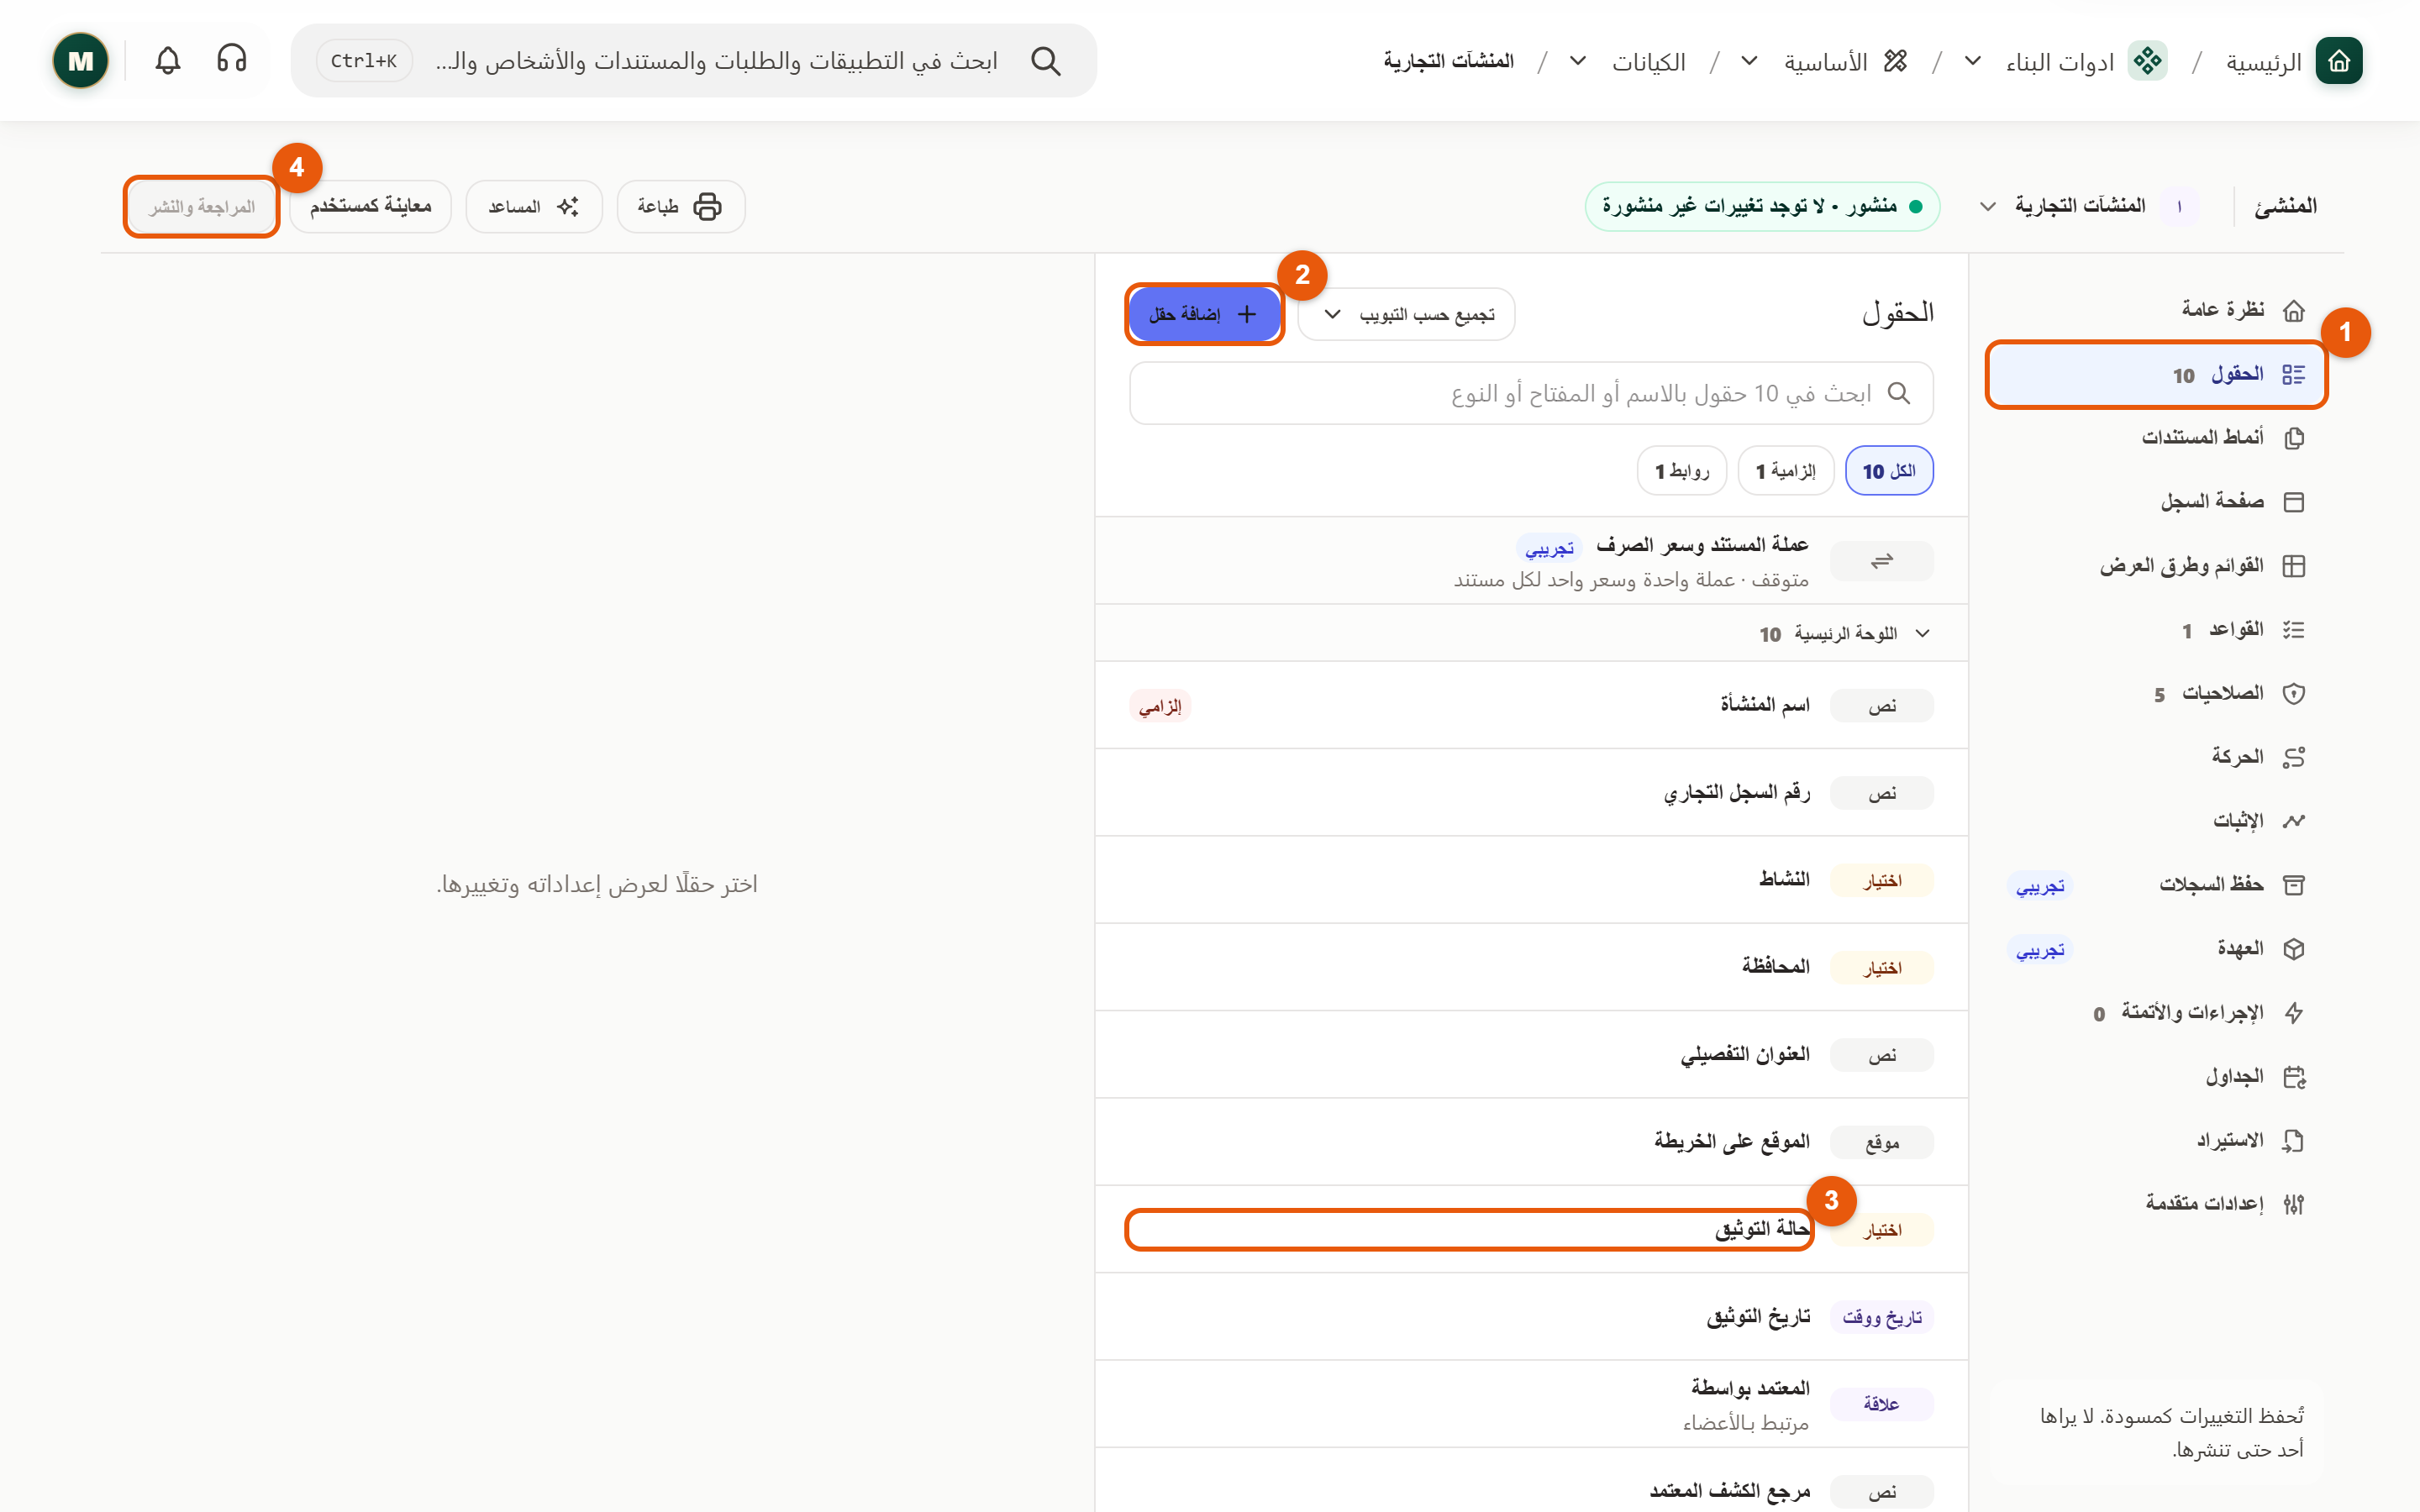
\includegraphics[width=0.95\linewidth]{assets/screens/entity-fields.png}
\caption{إعداد حقول المنشآت التجارية}
\label{fig:fields}
\shotnote{هذه شاشة تعديل نوع السجلات بعد إنشائه. ① «الحقول»: قائمة كل الحقول وأنواعها. ② «إضافة حقل»: أضف معلومة جديدة لاحقاً. ③ «حالة التوثيق»: مثال لحقل إضافي، وليس حالة سير الكشف. ④ «المراجعة والنشر»: يصبح متاحاً عندما توجد تعديلات في المسودة؛ تراجعها ثم تضغط «نشر» لتصل إلى المستخدمين.}
\end{figure}

\begin{enumerate}
\item اضغط على أي حقل في القائمة لتفتح إعداداته على اليسار: «التسمية» و«نص المساعدة» تحت «الأساسيات»، والخيارات تحت «إعدادات النوع»، و«إلزامي» تحت «القيمة» بخياراته «أبدًا» و«دائمًا» و«فقط عندما…».
\item بعد أي تعديل، اضغط «المراجعة والنشر». تفتح نافذة تعرض كل تغيير وبجانبه مربع اختيار. التغيير الذي تزيل علامته يبقى في المسودة.
\item إذا ظهر «أصلح … مشكلة للنشر» فاقرأ المشكلة وعالجها أولاً، مثل «في … خيار بلا قيمة مخزّنة».
\item اضغط «نشر 1 تغيير» أو «نشر … تغيير». تظهر «تم النشر.».
\end{enumerate}

\begin{rcwarn}[قبل حذف حقل أو تغيير نوعه]
تغيير نوع الحقل يمسح إعدادات نوعه القديم، مثل الخيارات. وحذف حقل فيه بيانات يعرض تحذيراً بعدد السجلات التي تحمل قيمة. لا تحذف حقلاً لأن اسمه غير مناسب: غيّر «التسمية» فقط. والنظام يمنع حذف الحقل الذي يسمّي السجلات، مثل «اسم المنشأة».
\end{rcwarn}

\textbf{تحقق:} يظهر «فرن الأمانة» باسمه في قائمة «المنشآت التجارية»، ويفتح ببياناته كلها. أعد فتحه وتأكد أن المحافظة والنشاط والموقع محفوظة. إذا ظهر بمعرّف بدل الاسم، فراجع «حقول الاسم المعروض».

\section{أنشئ استمارة الكشف}
\label{sec:build-form}

\textbf{لماذا؟} ملف المنشأة يحفظ معلوماتها الثابتة، أما «النموذج» فهو الاستمارة التي يعبئها الباحث في كل زيارة. للمنشأة الواحدة عدة كشوف عبر السنين، ولكل كشف إجاباته وقراره. النموذج قالب نصممه مرة واحدة؛ وكل استمارة يعبئها نور تسمى «إجابة».

\subsection{افهم أجزاء النموذج قبل أن تبدأ}

\begin{itemize}
\item \textbf{القسم:} عنوان يجمع أسئلة متقاربة، مثل «بيانات المنشأة».
\item \textbf{السؤال:} يجمع معلومة واحدة، مثل «ملاحظات الكشف».
\item \textbf{القاعدة:} تحدد متى يظهر السؤال، ومتى يكون مطلوباً، ومتى تكون إجابته صحيحة.
\item \textbf{الربط بالسجل:} يجلب بيانات المنشأة إلى الاستمارة، ويعيد التصحيح إلى ملفها.
\item \textbf{المسار:} ما يحدث للإجابة بعد الإرسال: من يراجعها وإلى أين تنتقل.
\end{itemize}

رتّب الاستمارة كما تحدث الزيارة: يختار الباحث المنشأة أولاً ويراجع بياناتها، ثم يكتب ما رآه وتوصيته، ثم يرفق الصور. لهذا يأتي سؤال المنشأة في أول الاستمارة دائماً.

\begin{table}[H]
\centering
\caption{حقول نافذة «إنشاء نموذج»}
\label{tab:form-create}
\begin{tabularx}{\linewidth}{R{3cm} R{2.4cm} Y}
\rcHeaderRow
\thh{الحقل} & \thh{هل هو مطلوب؟} & \thh{ماذا تكتب ولماذا}\\
اسم النموذج & \rec{} & «كشف منشأة تجارية لطلب سجل تجاري». يصبح عنوان الاستمارة. لا يُقبل اسم مستخدم لنموذج آخر.\\
كود النموذج & \req{} & \en{001}. يصبح المعرّف الدائم للنموذج ولا يتغير بعد الإنشاء. يحوّل النظام المسافات والرموز إلى \en{\_} والأحرف إلى صغيرة. إذا كان مستخدماً تظهر «يوجد نموذج برقم … بالفعل».\\
الوصف & \req{} & ما الغرض من الاستمارة، في 12 حرفاً وكلمتين على الأقل.\\
الاختصار المرجعي & \opt{} & حروف قصيرة مثل \en{KSHF} تميّز إجابات هذا النموذج. يجب ألا يستخدمه نموذج آخر. يختلف عن «كود النموذج».\\
إظهار في التنقل & \rec{} & مفعّل افتراضياً: يظهر النموذج في قائمة التطبيق.\\
التطبيق، قسم التطبيق & \req{} & «حماية المستهلك» ثم «السجلات».\\
\end{tabularx}
\end{table}

\begin{enumerate}
\item افتح «ادوات البناء» ← «النماذج»، واضغط «إنشاء نموذج».
\item املأ الحقول كما في الجدول، ثم اضغط «إنشاء». تظهر «تم إنشاء النموذج بنجاح» ويفتح المحرر.
\item يبدأ النموذج الجديد بقسم اسمه «القسم 1» فيه سؤال نصي اسمه «الحقل 1». سنعيد تسميتهما في الخطوة التالية بدل حذفهما.
\end{enumerate}

\begin{figure}[H]
\centering
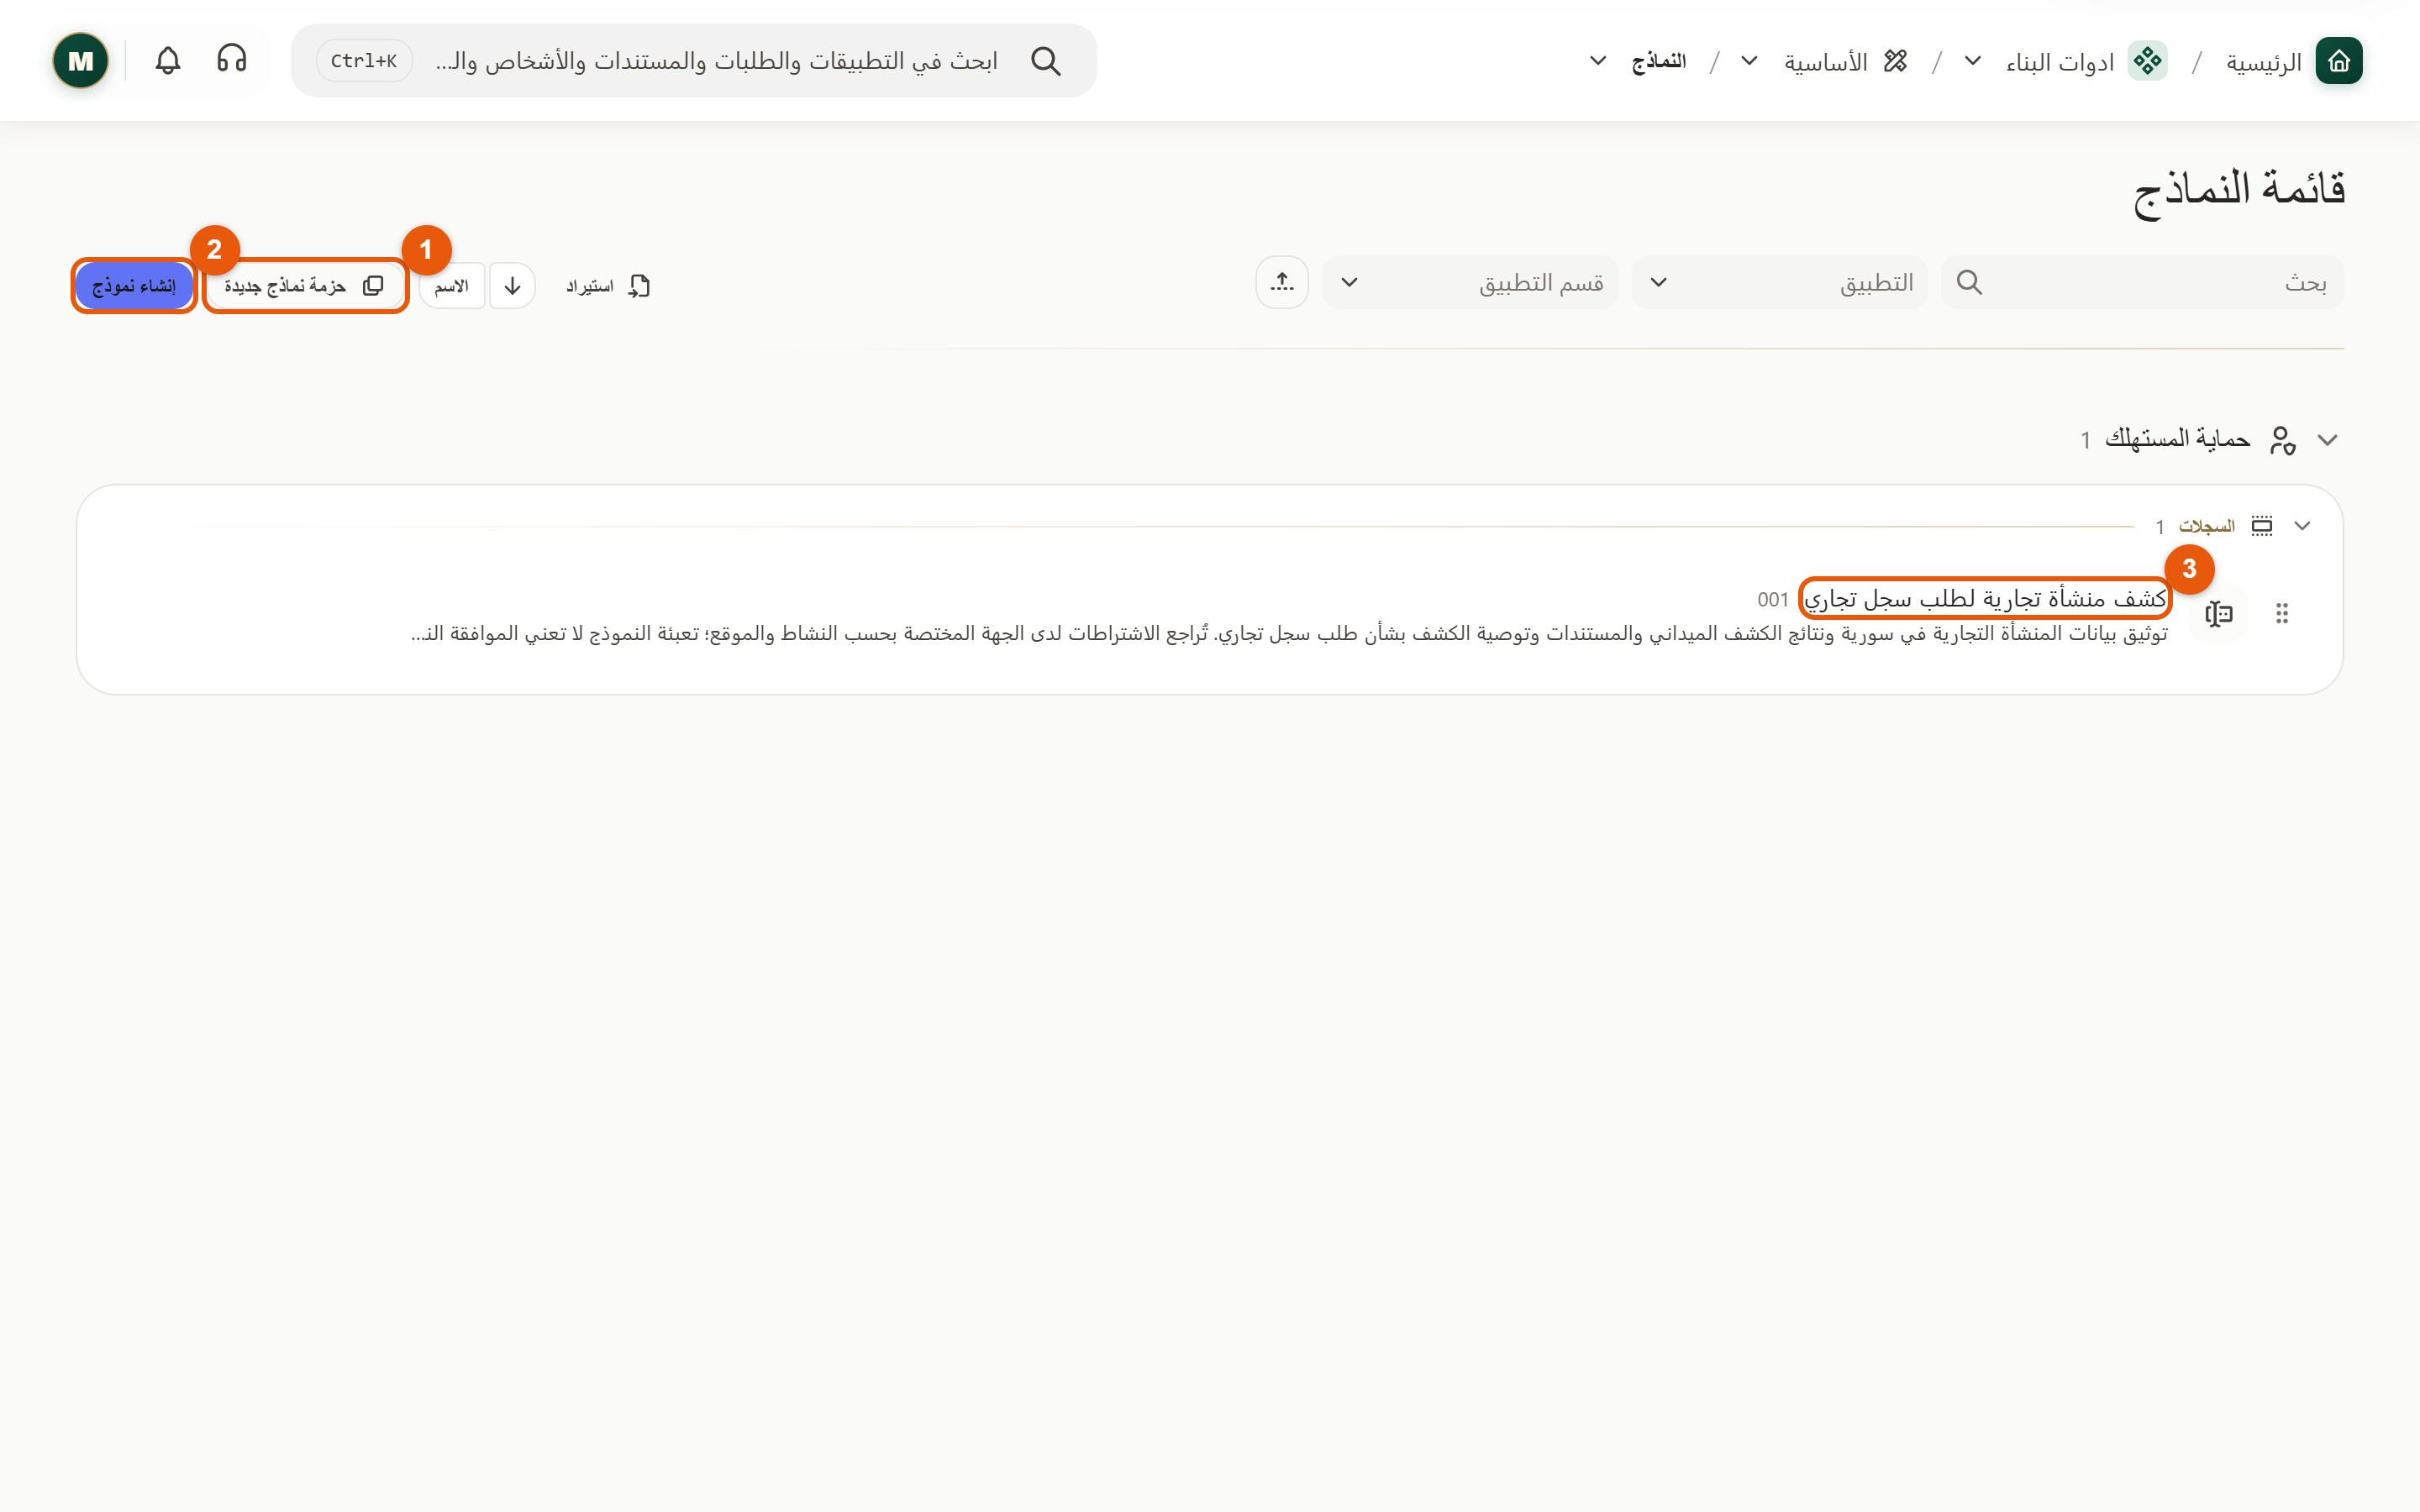
\includegraphics[width=0.95\linewidth]{assets/screens/forms-list.png}
\caption{إنشاء نموذج الكشف}
\label{fig:forms}
\shotnote{تبدأ الاستمارة من قائمة النماذج، ثم تفتح في المحرر. ① «حزمة نماذج جديدة»: تجمع عدة نماذج في طلب واحد؛ لا نحتاجها لهذا الكشف الواحد. ② «إنشاء نموذج»: ابدأ استمارة الكشف. ③ نموذج المثال باسمه وكوده.}
\end{figure}

\begin{rcnote}[الحفظ في المحرر تلقائي]
لا يوجد زر حفظ للأسئلة. كل تعديل يُحفظ وحده، وتظهر أعلى المحرر «جارٍ الحفظ» ثم «تم الحفظ». إذا ظهرت «فشلت المزامنة» فتحقق من اتصالك قبل متابعة العمل. ومع ذلك، ما تحفظه يبقى مسودة لا يراها الفريق حتى تضغط «نشر».
\end{rcnote}

\textbf{تحقق:} يظهر عنوان الكشف في المحرر، وتحته «القسم 1». النموذج لم يصل إلى الفريق بعد؛ سننشره بعد إكمال الأسئلة والربط والموافقة.

\subsection{ابنِ الأقسام والأسئلة واحداً واحداً}

عندما تضغط على قسم أو سؤال في المحرر، تفتح إعداداته في اللوحة الجانبية. في أعلى اللوحة «العنوان» ثم «الوصف». العنوان هو اسم المعلومة («ملاحظات الكشف»)، والوصف يشرح للباحث كيف يجيب («دوّن ما شاهدته وما يحتاج إلى تصحيح»). بجانب العنوان مفتاح رمادي يولّده النظام؛ يتغير مع العنوان حتى النشر الأول، ثم يثبت.

\begin{enumerate}
\item اضغط على «القسم 1» وغيّر «العنوان» إلى «بيانات المنشأة»، واكتب في «الوصف»: «اختر المنشأة ثم راجع بياناتها وصحح ما تغير». سنضيف سؤال المنشأة إلى هذا القسم لاحقاً، ثم نحذف «الحقل 1» إن لم نحتجه.
\item أضف قسماً ثانياً من زر «قسم» في شريط الإضافة، وسمّه «نتيجة الكشف».
\item داخل «نتيجة الكشف» افتح «اختر نوع الحقل» من شريط الإضافة، واختر «نص» من مجموعة «نص». يضيف هذا الزر سؤالاً \textbf{جديداً} في كل ضغطة؛ لتعديل سؤال موجود اضغط على السؤال نفسه.
\item اكتب عنوان السؤال «ملاحظات الكشف»، ووصفه «دوّن ما شاهدته في الزيارة وما يحتاج إلى تصحيح».
\item أضف سؤالاً من نوع «اختيار واحد» وسمّه «توصية القائم بالكشف». في مجموعة «الخيارات» اترك المصدر «يدوي»، واضغط «إضافة اختيار» أربع مرات: «التوصية بالموافقة»، و«استكمال نواقص قبل البت»، و«الحاجة إلى إعادة كشف»، و«عدم التوصية بالموافقة مع بيان الأسباب». تأكد أن «يختار المجيب» على «خيارًا واحدًا»، لأن الكشف ينتهي بتوصية واحدة.
\item أضف سؤالاً نصياً ثالثاً في القسم نفسه: «أسباب التوصية والنواقص المطلوب استكمالها». سنجعله مطلوباً بقاعدة في خطوة لاحقة.
\item أضف قسماً ثالثاً «المرفقات»، وفيه سؤال من نوع «ملف» من مجموعة «الملفات والوسائط»، عنوانه «صور الكشف ومستنداته». حدد في إعداده «الأنواع المقبولة» (مثل الصور وملفات \en{PDF}) و«أقصى حجم للملف» إذا أردت. اكتب في الوصف ما يجب تصويره.
\item أضف سؤال «رقم التواصل» إلى قسم «بيانات المنشأة» من النوع «هاتف أو رقم وطني». سنضبطه في الفقرة التالية.
\item رتّب الأسئلة بسحبها من مقبض السحب بجانبها. لنقل سؤال أو حذفه أو تكراره استخدم قائمة «إجراءات العنصر».
\end{enumerate}

\begin{rcnote}[توصية الباحث ليست القرار]
اختيار نور «التوصية بالموافقة» لا يعتمد الكشف. هو رأي يساعد ريم. القرار يبقى لريم في خطوة الموافقة.
\end{rcnote}

\subsection{اضبط السؤال: النوع والعرض والصيغة}

حدد سؤال «رقم التواصل»، ثم اتبع الأرقام في الصورة. اختر نوعه من ①، واضبط عرضه من ②، واجعل صيغته «رقم هاتف» عند ③ ورمز الدولة عند ④، ثم افتح «القواعد» عند ⑤. العرض يغيّر المساحة التي يأخذها السؤال على الشاشة، أما الصيغة فتحدد شكل الإجابة المقبولة.

\begin{figure}[H]
\centering
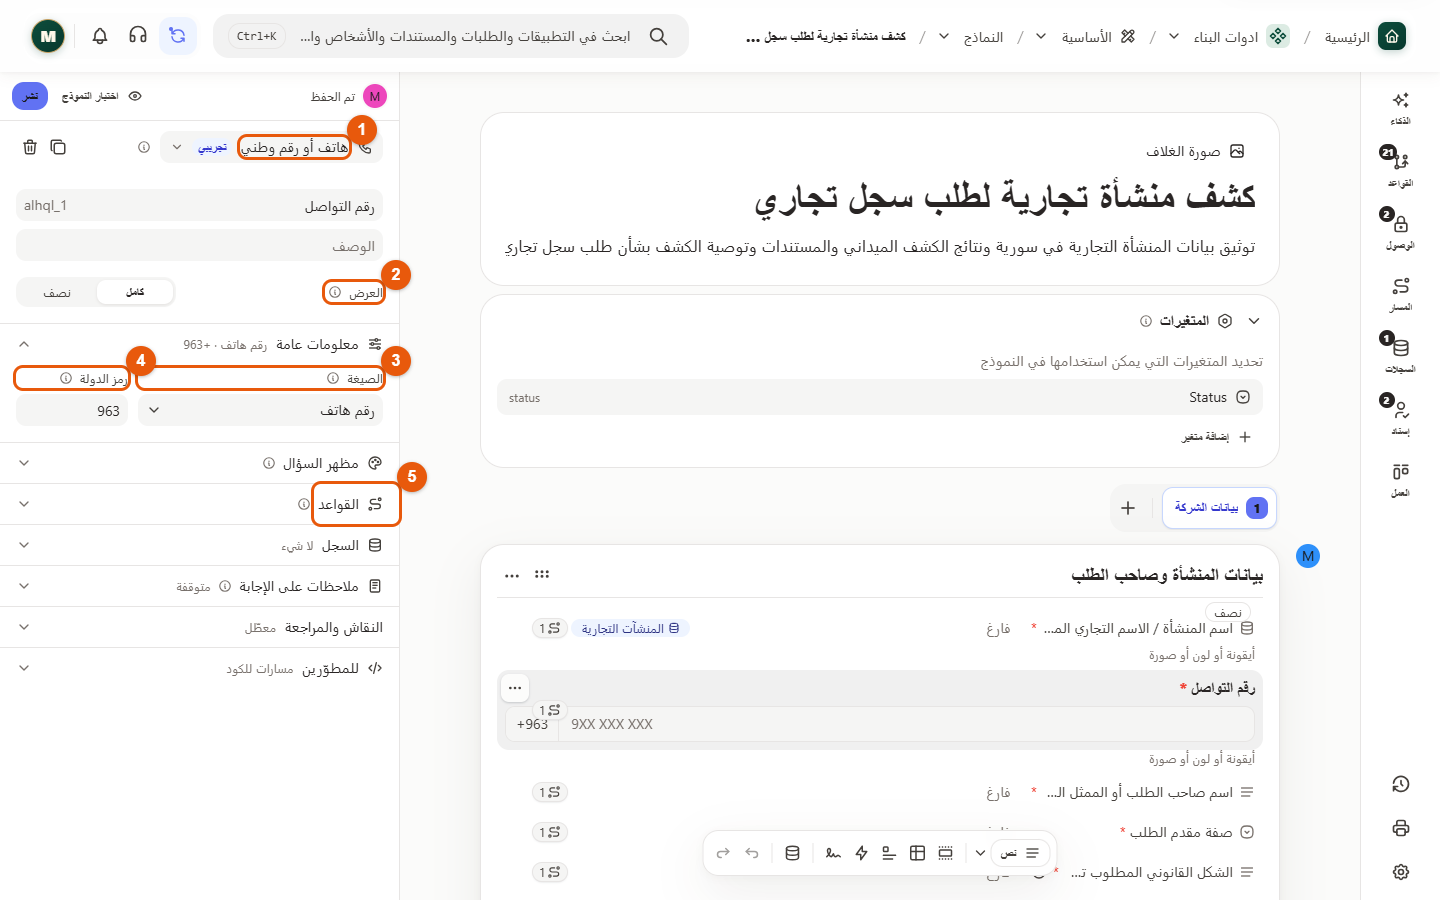
\includegraphics[width=0.95\linewidth]{assets/screens/org-question-settings.png}
\caption{إعداد نوع سؤال التواصل وعرضه وصيغته}
\label{fig:question-settings}
\shotnote{① نوع السؤال «هاتف أو رقم وطني». ② «العرض»: «كامل» يأخذ السطر كله، و«نصف» يضع السؤال بجانب سؤال آخر على الشاشات العريضة. ③ «الصيغة»: «رقم هاتف» يُفحص أثناء الكتابة ويُحفظ مع رمز الدولة. ④ رمز الدولة. ⑤ افتح قواعد السؤال لضبط الإلزام والظهور والتعديل.}
\end{figure}

\begin{table}[H]
\centering
\caption{خيارات «الصيغة» في السؤال النصي}
\label{tab:text-formats}
\begin{tabularx}{\linewidth}{R{3cm} Y}
\rcHeaderRow
\thh{الخيار} & \thh{متى تستخدمه}\\
أي نص & للملاحظات والوصف الحر. لا يفحص النظام شكل الإجابة.\\
رقم هاتف & لأرقام التواصل. يرفض الأرقام غير الصحيحة أثناء الكتابة.\\
رقم وطني & 11 رقماً، تُفحص أثناء الكتابة.\\
رقم سجل، بريد إلكتروني، رابط & لكل منها فحص يناسبه.\\
نمط & لصيغة خاصة. تكتب «النمط» و«الرسالة عند عدم التطابق» التي يراها الباحث.\\
\end{tabularx}
\end{table}

\subsection{قواعد السؤال: ستة إعدادات يجب أن تفهمها}

افتح مجموعة «القواعد» في إعدادات السؤال. اتبع ① لتحديد هل الإجابة مطلوبة، و② لظهور السؤال، و③ للسماح بتعديله. راجع ④ قبل وضع قيمة تلقائية، واترك ⑤ متوقفاً عندما تريد إجابة واحدة، واستخدم ⑥ لإضافة شرط صحة الإجابة.

\begin{figure}[H]
\centering
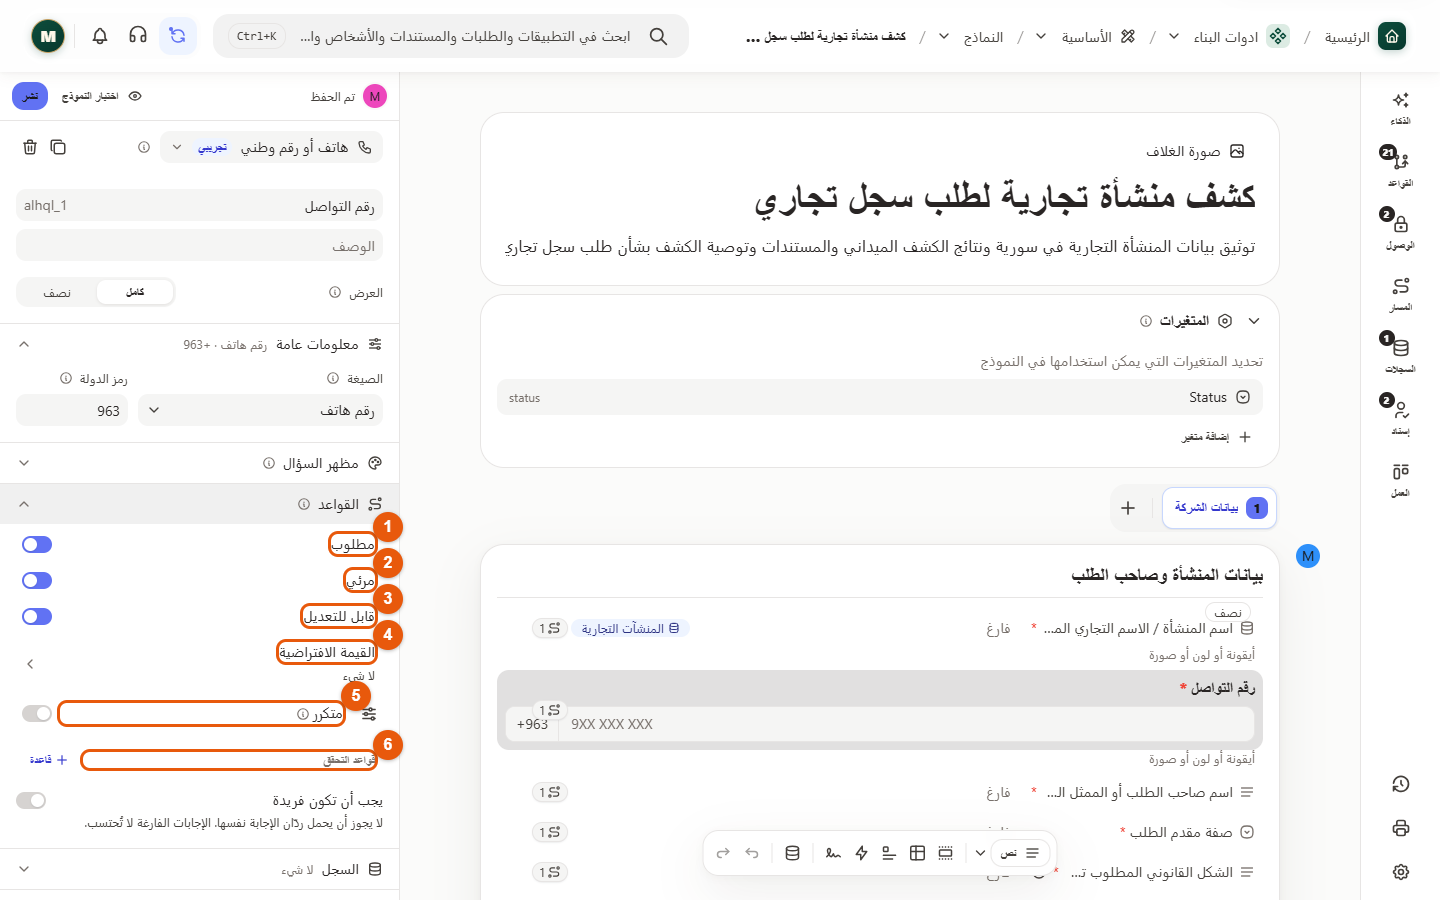
\includegraphics[width=0.95\linewidth]{assets/screens/org-question-rules.png}
\caption{قواعد السؤال: الإلزام والظهور والتعديل والقيمة الافتراضية}
\label{fig:question-rules}
\shotnote{① «مطلوب»: لا يُرسل الكشف وهذه الإجابة فارغة. ② «مرئي»: يظهر السؤال للباحث. ③ «قابل للتعديل»: إيقافه يقفل الإجابة. ④ «القيمة الافتراضية»: ما يُكتب في السؤال قبل أن يجيب الباحث. ⑤ «متكرر»: يسمح بعدة إجابات للسؤال نفسه. ⑥ «قواعد التحقق»: شروط تفحص صحة الإجابة.}
\end{figure}

\begin{table}[H]
\centering
\caption{معنى كل إعداد وقرارنا في الكشف}
\label{tab:question-settings}
\begin{tabularx}{\linewidth}{R{2.8cm} Y Y}
\rcHeaderRow
\thh{الإعداد} & \thh{معناه} & \thh{قرارنا في الكشف}\\
مطلوب & مفتاح: إما مطلوب دائماً، أو مطلوب بشرط (يظهر بجانبه «شرط»). & فعّله للمنشأة والتوصية. سؤال الأسباب مطلوب بشرط.\\
مرئي & يظهر السؤال أو يختفي، دائماً أو بشرط. & اترك كل أسئلة المثال ظاهرة.\\
قابل للتعديل & إيقافه يجعل السؤال للقراءة فقط. & لا تقفل سؤالاً مطلوباً لا يملؤه شيء، وإلا لن يُرسل الكشف.\\
القيمة الافتراضية & قيمة تُكتب في السؤال قبل أن يجيب الباحث، ويبقى قادراً على تغييرها. & لا تضع توصية افتراضية: دع الباحث يختار بنفسه.\\
متكرر & يحوّل السؤال إلى قائمة إجابات. & اتركه متوقفاً لكل الأسئلة، خصوصاً المرتبطة بحقل واحد في المنشأة.\\
قواعد التحقق & شروط على قيمة الإجابة، مع رسالة توضح الخطأ. & أضفها فقط عندما توجد قاعدة عمل واضحة.\\
يجب أن تكون فريدة & يمنع أن تحمل إجابتان القيمة نفسها. & لا نحتاجه هنا.\\
\end{tabularx}
\end{table}

\begin{rcnote}[مستويات قاعدة التحقق]
عند إضافة قاعدة تحقق بزر «+ قاعدة» تختار «المستوى». «خطأ» يمنع الإرسال تماماً. «تنبيه» يسمح بالإرسال بعد أن يكتب الباحث سبباً. «ملاحظة للمراجع» يراها المدقق وحده. «تلميح» نص رمادي لا يمنع شيئاً. ثم تكتب «الرسالة» التي يراها الباحث، وتختار «متى» تُفحص: «أثناء الكتابة» أو «عند مغادرة الصفحة» أو «عند الإرسال».
\end{rcnote}

الاختيار يختلف عن النص: قائمة الخيارات تمنع كتابة الشيء نفسه بعدة صيغ. والرقم يختلف عن المعرّف: رقم السجل التجاري نحفظه كنص لأننا لا نحسب به.

\textbf{تحقق:} اضغط «اختبار النموذج» أعلى المحرر. اترك التوصية فارغة وحاول الإرسال؛ يجب أن تظهر «أجب عن الأسئلة المطلوبة» ويُمنع الإرسال. أكمل التوصية وتأكد من زوال التنبيه. جرّب أيضاً كتابة رقم هاتف ناقص، ورفع صورة وفتحها.

\subsection{قواعد الظهور والإلزام: متى نحتاجها؟}

قاعدة الظهور تجيب: متى يحتاج الباحث أن يرى هذا السؤال؟ وقاعدة الإلزام تجيب: متى يجب أن يجيب عنه؟ في مثالنا: عندما يوصي نور بالموافقة لا نحتاج أسباباً، أما عند التوصيات الثلاث الأخرى فنحتاج أن يشرح السبب. لذلك نجعل سؤال الأسباب مطلوباً بشرط.

\begin{table}[H]
\centering
\caption{أنواع القواعد في نافذة القاعدة}
\label{tab:rule-kinds}
\begin{tabularx}{\linewidth}{R{3cm} Y}
\rcHeaderRow
\thh{التبويب} & \thh{خياراته}\\
إظهار أو إخفاء & «يظهر عندما» أو «يُخفى عندما» أو «دائماً».\\
إلزام & «مطلوب عندما» أو «مطلوب دائماً». لجعل السؤال غير مطلوب أوقف «مطلوب» في لوحة السؤال.\\
قفل التعديل & «مقفل عندما» أو «قابل للتعديل فقط عندما» أو «مقفل دائماً».\\
قيمة افتراضية، حساب، تحقق & قيمة البداية، أو قيمة تُحسب من إجابات أخرى، أو شرط صحة.\\
\end{tabularx}
\end{table}

\begin{enumerate}
\item حدد سؤال «أسباب التوصية والنواقص المطلوب استكمالها»، ثم اضغط صف «مطلوب» في «القواعد». تفتح نافذة القاعدة على تبويب «إلزام» عند ① في الصورة. اختر «مطلوب عندما».
\item تحت «عندما» أضف شرطاً: اختر سؤال «توصية القائم بالكشف»، والعامل «هو»، والخيار «استكمال نواقص قبل البت».
\item اضغط «+ أو» وأضف شرطاً ثانياً بالخيار «الحاجة إلى إعادة كشف»، ثم شرطاً ثالثاً بالخيار «عدم التوصية بالموافقة مع بيان الأسباب».
\item بعد إضافة شرطين أو أكثر يظهر «طريقة جمع الشروط». اختر «أيّ» عند ②: يكفي تحقق شرط واحد. («كل» تعني أن تتحقق جميعها معاً، وهذا مستحيل هنا لأن التوصية واحدة. و«لا شيء مما يلي» تعني ألا يتحقق أي منها.)
\item تأكد أن «ثم ألزم» عند ④ يشير إلى سؤال الأسباب، ثم اضغط «حفظ في المسودة» عند ⑤.
\end{enumerate}

\begin{figure}[H]
\centering
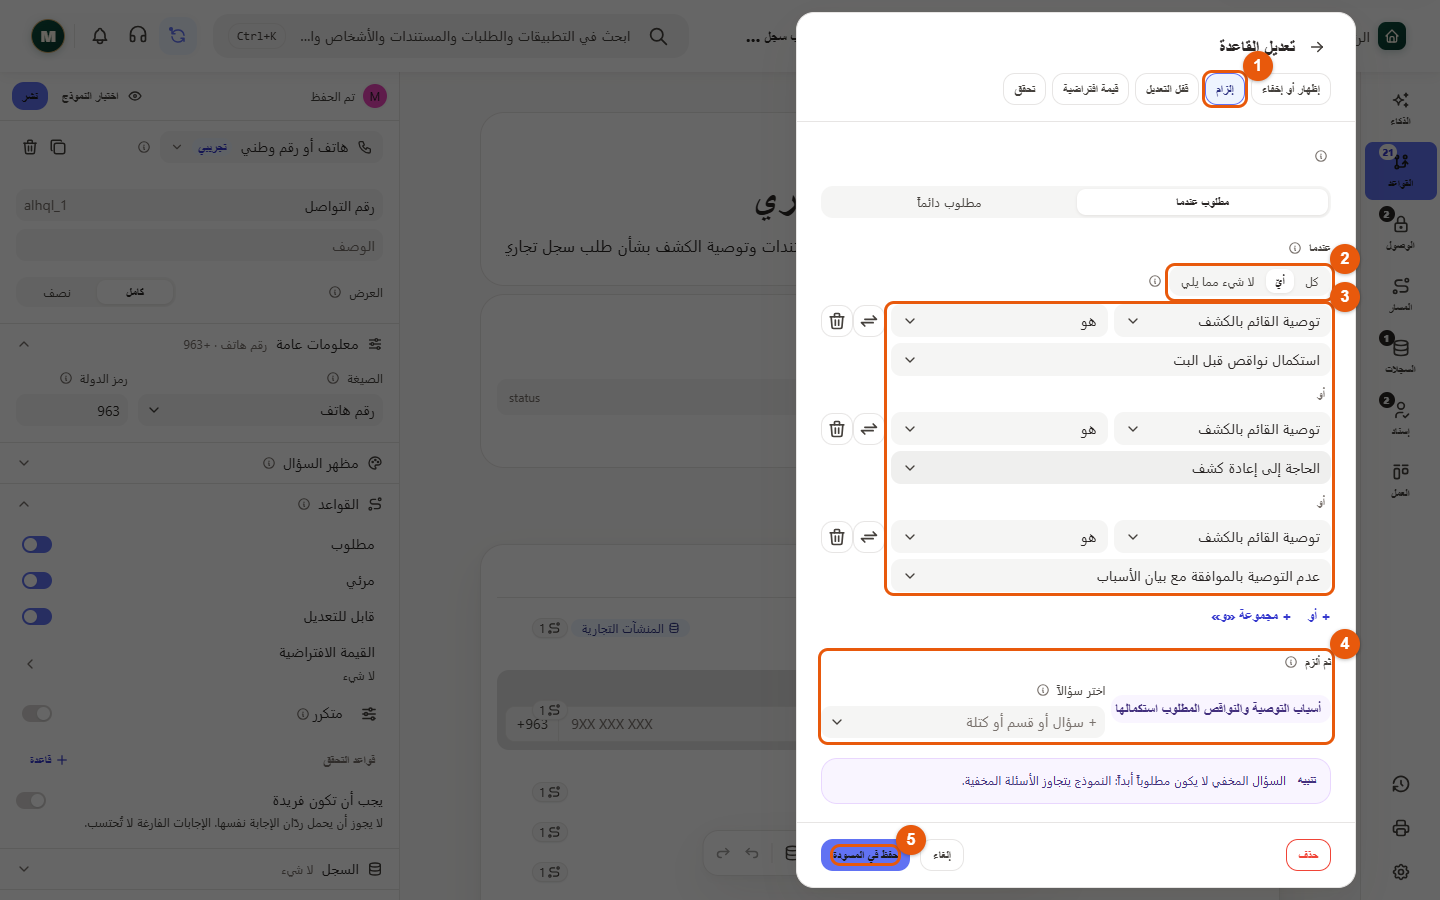
\includegraphics[width=0.95\linewidth]{assets/screens/org-required-condition.png}
\caption{إلزام أسباب التوصية عند الاستكمال أو إعادة الكشف أو عدم الموافقة}
\label{fig:required-condition}
\shotnote{① نوع القاعدة «إلزام». ② «أيّ»: تحقق واحد من الشروط يكفي. ③ شروط التوصية الثلاثة المتصلة بـ«أو». ④ السؤال الذي يصبح مطلوباً عند تحقق الشرط. ⑤ «حفظ في المسودة»: تُحفظ القاعدة في المسودة، ثم تختبرها قبل نشر النموذج.}
\end{figure}

\begin{table}[H]
\centering
\caption{العوامل التي ستراها في الشروط}
\label{tab:operators}
\begin{tabularx}{\linewidth}{R{3cm} Y}
\rcHeaderRow
\thh{نوع السؤال} & \thh{العوامل المتاحة}\\
اختيار واحد & «هو»، «ليس»، «أحد» (أي واحد من عدة خيارات)، «ليس أيًّا من»، «فارغ»، «معبّأ».\\
نص & «هو»، «ليس»، «يتضمن»، «لا يتضمن»، «يبدأ بـ»، «ينتهي بـ»، «فارغ»، «معبّأ».\\
رقم & «أكبر من»، «على الأقل»، «أقل من»، «على الأكثر»، وغيرها.\\
تاريخ & «قبل»، «بعد»، «قبل اليوم»، «خلال الأيام الماضية»، وغيرها.\\
\end{tabularx}
\end{table}

\begin{rcnote}[طريقة أقصر للشرط نفسه]
بدل ثلاثة شروط متصلة بـ«أو»، يمكنك كتابة شرط واحد بالعامل «ليس» والخيار «التوصية بالموافقة». النتيجة واحدة. لكن انتبه: هذا الشرط يتحقق أيضاً عندما تكون التوصية فارغة، فيظهر سؤال الأسباب مطلوباً قبل أن يختار الباحث توصية. الطريقة الأولى أوضح للمبتدئ.
\end{rcnote}

\begin{rcwarn}[السؤال المخفي لا يكون مطلوباً]
النموذج يتجاوز الأسئلة المخفية ولا يطلبها أبداً. لذلك إذا أخفيت سؤال الأسباب ثم جعلته مطلوباً بشرط، فلن يُطلب ما دام مخفياً. في مثالنا نترك سؤال الأسباب ظاهراً دائماً. والإخفاء ليس وسيلة لحماية بيانات سرية؛ الصلاحيات هي التي تحمي البيانات.
\end{rcwarn}

\textbf{تحقق:} داخل نافذة القاعدة يوجد جزء «جرّبها»: اختر في «إجابات للتجربة» كل توصية، واقرأ «النتيجة»: «مطلوب» للتوصيات الثلاث و«اختياري» للموافقة. ثم افتح «اختبار النموذج»، واختر «عدم التوصية بالموافقة مع بيان الأسباب»، واترك الأسباب فارغة وحاول الإرسال؛ يجب أن يمنعك النموذج. اكتب السبب وأعد المحاولة.

\subsection{القيم الافتراضية والمتغيرات دون خلطها بالربط}

القيمة الافتراضية قيمة بداية ثابتة أو محسوبة. أما بيانات المنشأة فتأتي من الملف الذي يختاره الباحث، عبر الربط الذي سنضبطه بعد قليل. لذلك لا تكتب عنوان الفرن كقيمة افتراضية: لو فعلت لظهر عنوان الفرن نفسه في كشف أي منشأة أخرى.

عند فتح «القيمة الافتراضية» تختار نوع «القيمة»:

\begin{itemize}
\item «ثابتة»: قيمة تكتبها بنفسك. في السؤال النصي اكتب النص كما هو، والنظام يضيف علامتي التنصيص. لا تحتاج إلى التنصيص إلا إذا كتبت في «التعديل كتعبير»، مثل \en{"KSHF"}. وفي سؤال الاختيار اكتب \textbf{قيمة الخيار المخزّنة} لا نصه العربي.
\item «من سؤال»: انسخ إجابة سؤال آخر.
\item «مَن / متى»: مثل «من يعبّئ النموذج» أو «اليوم / الآن». مفيد لسؤال «تاريخ الزيارة».
\item «حساب» و«معادلة» و«إذا… وإلا»: قيم محسوبة لمن يحتاجها.
\end{itemize}

ثم تختار «السلوك»: «قيمة أولى فقط» تضع القيمة مرة واحدة ويستطيع الباحث تغييرها، و«يُحسب دائماً (مقفل)» يعيد حسابها مع كل تغيير ويقفل السؤال.

\begin{rcnote}[ما المتغيرات؟]
في الشريط الجانبي «المتغيرات»: قيم داخلية لا يراها الباحث، تستخدمها القواعد أو تُمرَّر إلى النموذج عند فتحه. لكل نموذج متغير اسمه \en{status} يحفظ حالته ولا يُحذف. لا تحتاج إلى إنشاء متغير لكل سؤال أو لربط المنشأة.
\end{rcnote}

\textbf{تحقق:} لا يحمل النموذج توصية مسبقة، ولا عنواناً ثابتاً لمنشأة بعينها. وكل قيمة تلقائية تعرف مصدرها.

\section{أضف «سؤال سجل»: أي منشأة سنكشف عليها؟}
\label{sec:build-record-question}

\textbf{ما معنى سؤال سجل؟} هو سؤال يختار فيه الباحث سجلاً من نوع السجلات الذي أنشأناه. في مثالنا يختار «فرن الأمانة» من قائمة «المنشآت التجارية». النظام لا يحفظ اسم الفرن كنص، بل يحفظ رابطاً إلى ملفه.

\textbf{لماذا نحتاجه؟} لو كتب الباحث اسم الفرن في سؤال نصي، فلن يعرف النظام أي ملف يقصد، وقد يكتبه بصيغة مختلفة كل مرة. سؤال السجل هو الذي يربط الكشف بالملف الصحيح، ويسمح بجلب بياناته وتحديثها بعد الاعتماد.

\begin{enumerate}
\item داخل محرر النموذج، اضغط «السجلات» في الشريط الجانبي. تفتح لوحة عنوانها «السجلات».
\item اضغط «سؤال سجل» عند العلامة ① في الصورة. يُضاف سؤال جديد اسمه «سجل».
\item في إعدادات السؤال افتح «نوع السجل» واختر «المنشآت التجارية». هذا يحدد القائمة التي سيختار منها الباحث.
\item غيّر عنوان السؤال إلى «اسم المنشأة / الاسم التجاري المقترح»، وفعّل «مطلوب» في «القواعد».
\item تأكد أن «يختار المجيب» على «خيارًا واحدًا». سؤال السجل يحتاج اختياراً واحداً؛ وإلا ظهرت «سؤال السجل يحتاج اختياراً واحداً».
\item في «السجل» اختر «موجود فقط». انظر الجدول لمعنى الخيارات الأربعة.
\item اسحب السؤال إلى أول قسم «بيانات المنشأة»، قبل الأسئلة التي ستجلب بياناته. لا تضعه داخل قسم «متكرر».
\end{enumerate}

\begin{table}[H]
\centering
\caption{خيارات «السجل» في سؤال السجل}
\label{tab:record-modes}
\begin{tabularx}{\linewidth}{R{3cm} Y}
\rcHeaderRow
\thh{الخيار} & \thh{معناه ومتى تختاره}\\
موجود فقط & يختار الباحث منشأة موجودة ولا يستطيع إنشاء منشأة جديدة. \textbf{اختيارنا}، لأن الكشف يكون على منشأة مسجلة.\\
موجود أو جديد & يختار منشأة موجودة، أو يضغط «غير موجود في القائمة: سجل جديد». مناسب لكشف منشآت لم تُسجل بعد.\\
جديد دائماً & كل إجابة تُنشئ منشأة جديدة. مناسب لاستمارة تسجيل منشأة، لا لكشف.\\
يحدده شرط & جديد أو موجود بحسب إجابة أخرى.\\
\end{tabularx}
\end{table}

\begin{table}[H]
\centering
\caption{إعدادات أخرى في سؤال السجل}
\label{tab:record-question-more}
\begin{tabularx}{\linewidth}{R{3.4cm} Y}
\rcHeaderRow
\thh{الإعداد} & \thh{معناه وقرارنا}\\
اعرض القائمة على شكل & «قائمة منسدلة» أو «قائمة» أو «بطاقات» أو «جدول». القائمة المنسدلة أبسط للباحث.\\
أي السجلات & شروط تحدد المنشآت التي تظهر للاختيار، مثل منشآت محافظة واحدة. نتركها «لا شروط».\\
مستوى الوصول & «عرض جميع الخيارات» أو «حسب صلاحيات المستخدم». الثاني يعرض للباحث المنشآت التي يحق له رؤيتها فقط.\\
الاختيار التلقائي & «اختره عندما يطابق سجل واحد فقط». مفيد مع الشروط؛ لا نحتاجه هنا.\\
طريقة الكتابة & «مباشرة» تكتب الإجابات في الملف كما هي. «كتعديل محكوم» يطلب سبباً لكل تغيير. نتركها «مباشرة».\\
\end{tabularx}
\end{table}

\begin{figure}[H]
\centering
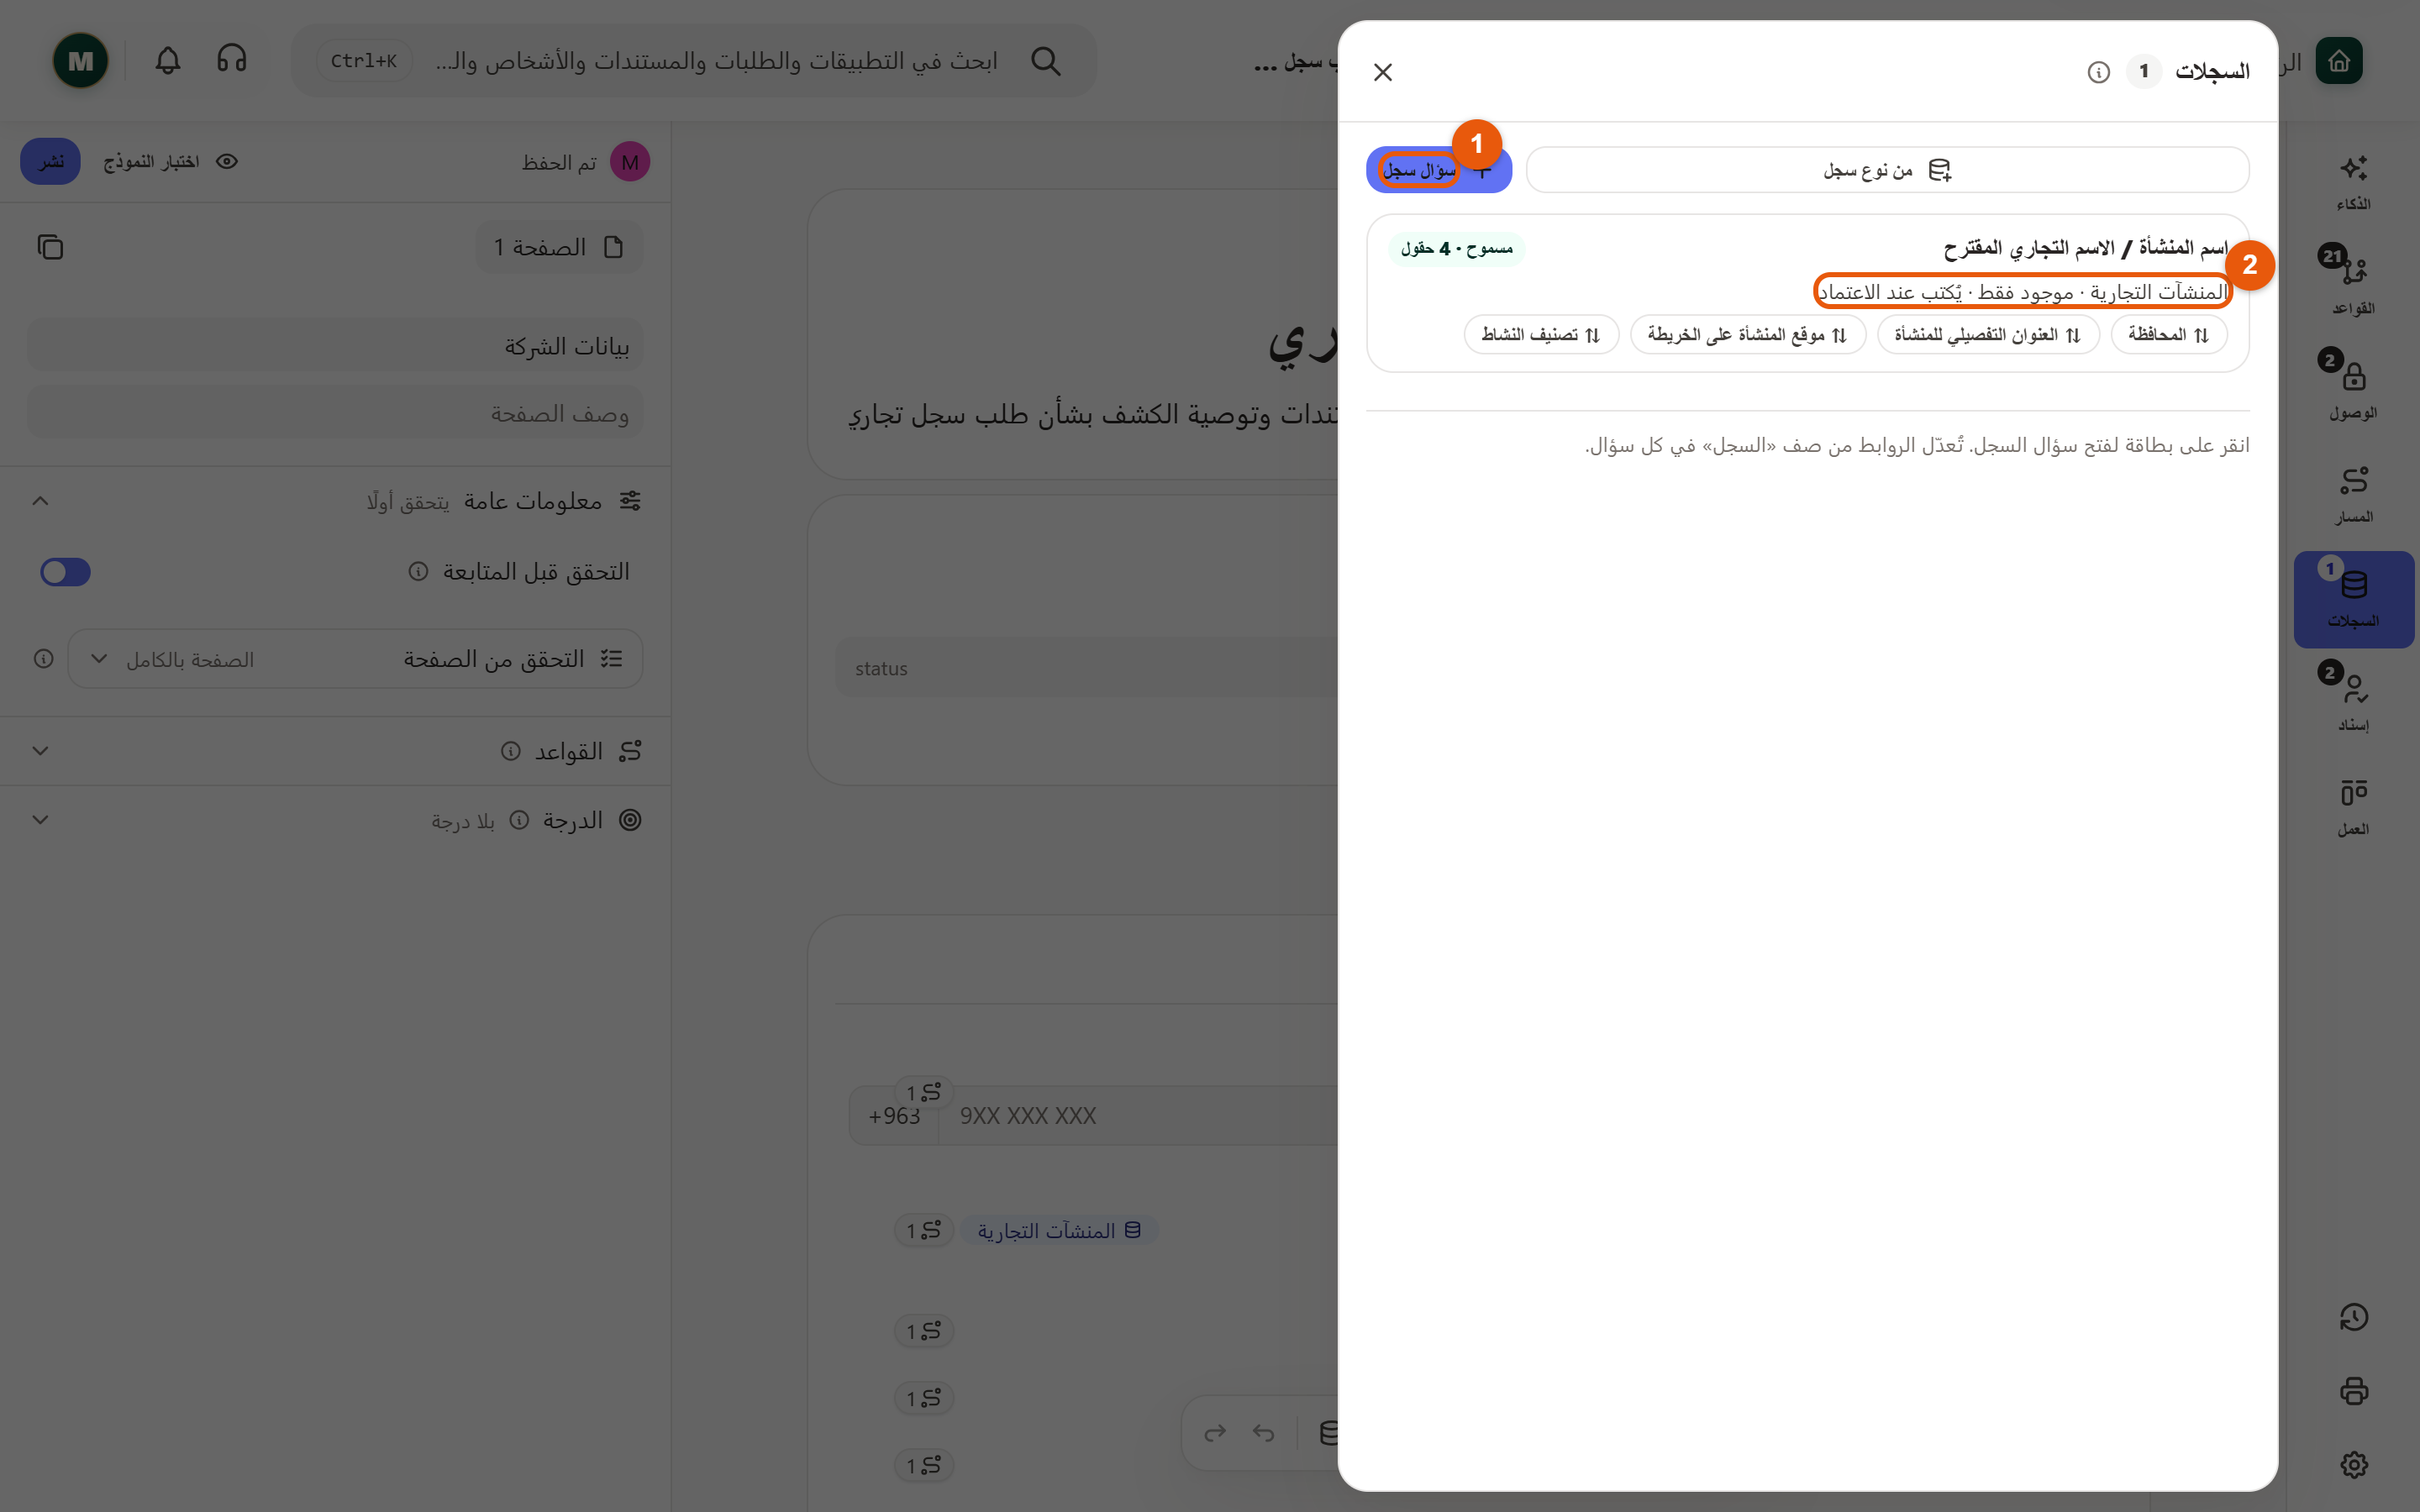
\includegraphics[width=0.95\linewidth]{assets/screens/form-records.png}
\caption{اختيار المنشأة وربط حقولها بالكشف}
\label{fig:record-question}
\shotnote{بطاقة السجل تجمع اختيار المنشأة والحقول المرتبطة بملفها. ① «سؤال سجل»: أضف سؤال اختيار المنشأة. ② ملخص البطاقة: نوع السجل «المنشآت التجارية»، و«موجود فقط» أي يُختار ملف قائم، و«يُكتب عند الاعتماد» أي تنتظر التغييرات المرتبطة الموافقة قبل تحديث ملف المنشأة.}
\end{figure}

\textbf{تحقق:} اضغط «اختبار النموذج»، وافتح سؤال المنشأة. يجب أن تتمكن من اختيار «فرن الأمانة». إذا لم يظهر، تأكد من «نوع السجل» ومن صلاحية قراءة المنشآت. وإذا ظهر في البطاقة «غير مستخدم: تحقق من نوع السجل والاختيار الواحد والمكان.» فراجع هذه الثلاثة بالترتيب.

\section{اجلب بيانات المنشأة إلى أسئلة الكشف}
\label{sec:build-links}

\textbf{لماذا؟} بعد اختيار الفرن نريد أن تظهر محافظته وعنوانه ونشاطه وموقعه تلقائياً، كي لا يعيد الباحث كتابتها. وإذا وجد في الزيارة معلومة تغيّرت، يصححها في الكشف، وينتقل التصحيح إلى ملف الفرن بعد اعتماد ريم.

«سؤال سجل» يختار المنشأة. أما «من نوع سجل» فيضيف أسئلة مأخوذة من حقول تلك المنشأة. الأول يحدد \textbf{أي منشأة}، والثاني يحدد \textbf{أي معلومات نأخذ منها}.

\subsection{الخطوة 1 من المعالج: «نوع السجل»}

افتح «السجلات» داخل النموذج، واضغط «من نوع سجل». يفتح معالج «إضافة أسئلة من نوع سجل» بأربع خطوات: «نوع السجل» ثم «الحقول» ثم «القوائم المرتبطة» ثم «مراجعة». اكتب «المنشآت التجارية» في البحث ① واخترها. على اليسار يظهر «السجل الذي تُربط به الأسئلة»: اختر بطاقة سؤال المنشأة الذي أضفته عند ②. الخيار ③ «سؤال سجل جديد» ينشئ سؤال اختيار ثانياً، و④ «بلا سؤال سجل» يضيف أسئلة عادية بلا ربط؛ لا تستخدمهما هنا. اضغط ⑤ للانتقال إلى الحقول.

\begin{figure}[H]
\centering
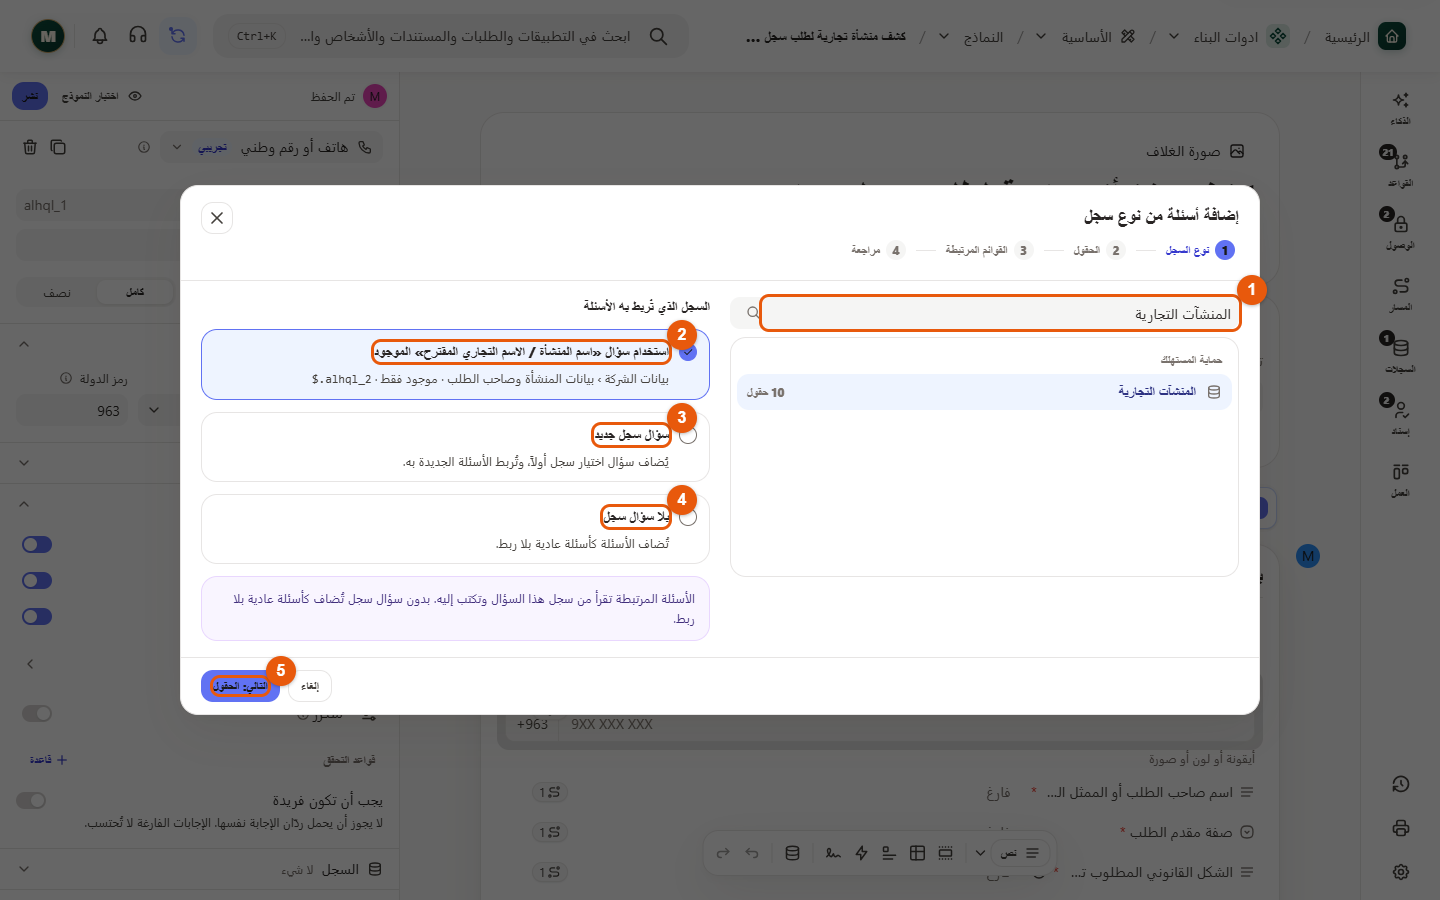
\includegraphics[width=0.95\linewidth]{assets/screens/org-record-source.png}
\caption{تحديد نوع السجلات والسؤال الذي يختار المنشأة}
\label{fig:record-source}
\shotnote{① البحث عن نوع السجلات. ② «استخدام سؤال … الموجود»: اربط الأسئلة بسؤال المنشأة الذي أنشأته. ③ «سؤال سجل جديد»: لاختيار سجل مستقل آخر. ④ «بلا سؤال سجل»: أسئلة عادية بلا ربط. ⑤ الانتقال إلى «الحقول».}
\end{figure}

\subsection{الخطوة 2: «الحقول» — ثلاثة أعمدة تقرر كل شيء}

في شاشة الحقول صف لكل حقل في «المنشآت التجارية». حدد صفوف «المحافظة» و«العنوان التفصيلي» و«الموقع على الخريطة» و«النشاط» من مربع الاختيار عند ①. ثم اضبط لكل صف ثلاثة أعمدة: «في النموذج» ②، و«الربط» ③، و«التعبئة المسبقة» ④.

\begin{figure}[H]
\centering
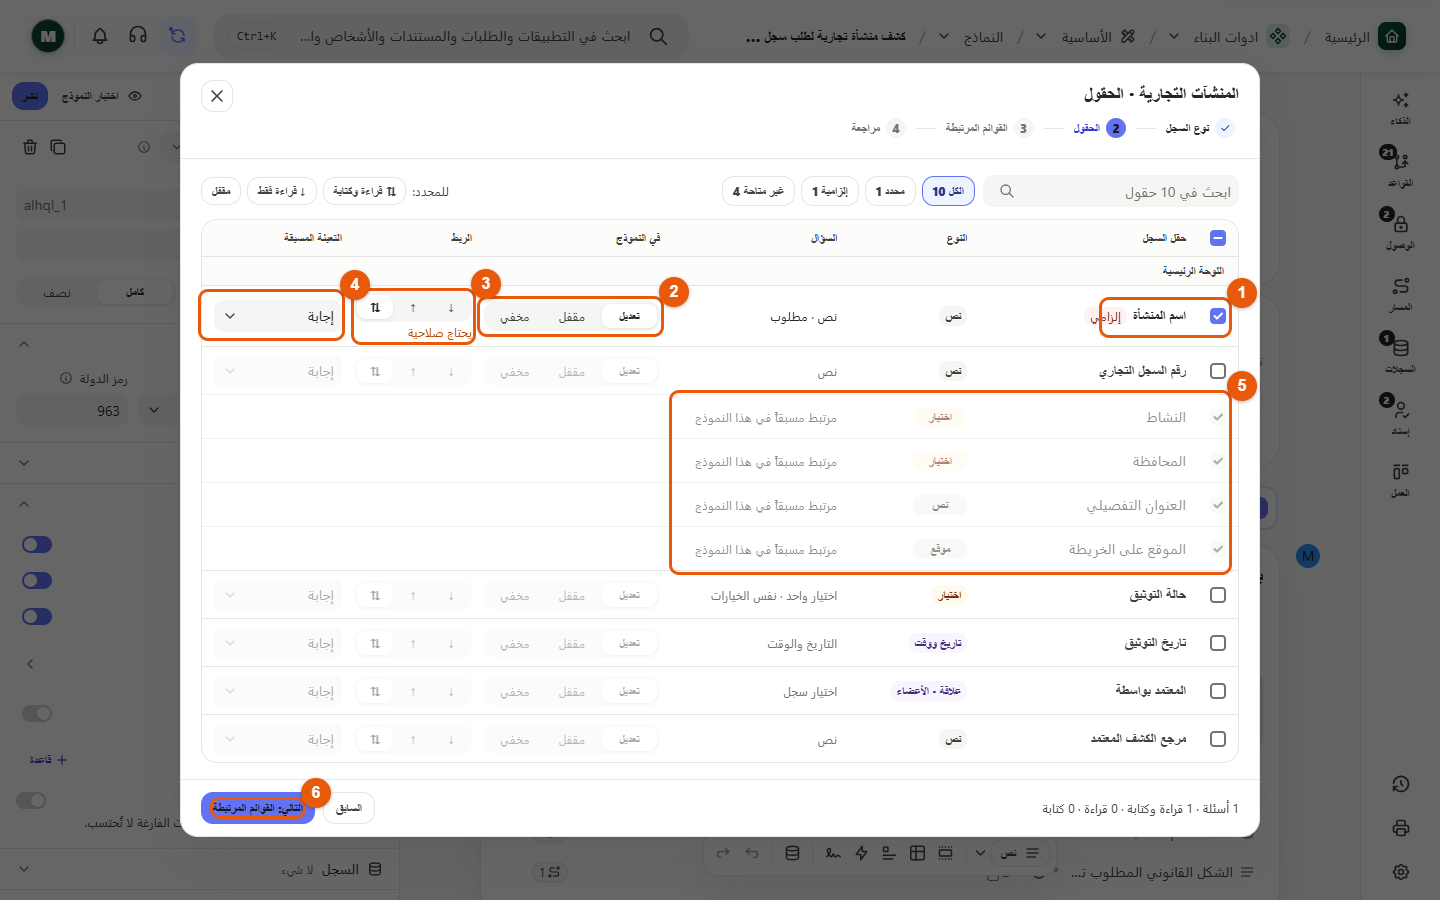
\includegraphics[width=0.95\linewidth]{assets/screens/org-record-fields.png}
\caption{اختيار الحقول واتجاه الربط وطريقة عرض الإجابة}
\label{fig:record-fields}
\shotnote{① تحديد الحقل؛ الاسم المحدد هنا يوضح مكان الاختيار. ② «في النموذج»: «تعديل» أو «مقفل» أو «مخفي». ③ «الربط»: ↓ قراءة، ↑ كتابة، ⇅ الاثنان؛ وتظهر تحته «يحتاج صلاحية» عندما تحتاج الكتابة إذناً. ④ «التعبئة المسبقة». ⑤ هذه الحقول الأربعة «مرتبط مسبقاً في هذا النموذج»، أي رُبطت من قبل، وليست حقولاً جديدة. ⑥ متابعة المعالج إلى «القوائم المرتبطة» ثم «مراجعة».}
\end{figure}

\begin{table}[H]
\centering
\caption{عمود «في النموذج»: كيف يرى الباحث السؤال؟}
\label{tab:in-form}
\begin{tabularx}{\linewidth}{R{2.4cm} Y}
\rcHeaderRow
\thh{الخيار} & \thh{معناه}\\
تعديل & يرى الباحث القيمة ويستطيع تصحيحها. \textbf{اختيارنا} للحقول الأربعة.\\
مقفل & يرى القيمة ولا يستطيع تغييرها. يجعل الربط «قراءة» وحدها تلقائياً. مناسب لرقم السجل التجاري إذا أردت عرضه فقط.\\
مخفي & لا يرى الباحث السؤال، لكنه موجود في الإجابة.\\
\end{tabularx}
\end{table}

\begin{table}[H]
\centering
\caption{عمود «الربط»: في أي اتجاه تنتقل القيمة؟}
\label{tab:link-modes}
\begin{tabularx}{\linewidth}{R{3cm} Y}
\rcHeaderRow
\thh{السهم} & \thh{ما الذي يحدث؟}\\
↓ قراءة & يجلب القيمة من ملف المنشأة إلى الكشف، ولا يغيّر الملف أبداً.\\
↑ كتابة & يرسل إجابة الكشف إلى حقل المنشأة، دون أن يجلب القيمة القديمة أولاً.\\
⇅ قراءة وكتابة & يجلب القيمة أولاً، ثم يحفظ التصحيح في الملف في موعد الكتابة. \textbf{اختيارنا} للحقول الأربعة.\\
\end{tabularx}
\end{table}

\begin{table}[H]
\centering
\caption{عمود «التعبئة المسبقة»: ماذا يرى الباحث عند فتح الاستمارة؟}
\label{tab:prefill}
\begin{tabularx}{\linewidth}{R{3cm} Y}
\rcHeaderRow
\thh{الخيار} & \thh{معناه}\\
إجابة & تُكتب القيمة الحالية في خانة الإجابة، ويعدّلها الباحث إن لزم. \textbf{اختيارنا}.\\
مرجع فقط & تظهر القيمة الحالية بجانب السؤال للمقارنة، وتبقى الخانة فارغة ليكتب الباحث ما شاهده.\\
بلا تعبئة & لا تُعرض القيمة الحالية.\\
\end{tabularx}
\end{table}

\begin{rcnote}[أزرار سريعة لكل الصفوف المحددة]
فوق الجدول، بجانب «للمحدد:»، ثلاثة أزرار تطبق اختياراً واحداً على كل الصفوف المحددة: «⇅ قراءة وكتابة» و«↓ قراءة فقط» و«مقفل». هي اختصار فقط؛ النتيجة نفسها لو ضبطت كل صف بيدك.
\end{rcnote}

\subsection{الخطوتان 3 و4: «القوائم المرتبطة» و«مراجعة»}

\begin{enumerate}
\item في «القوائم المرتبطة» يعرض المعالج سجلات أخرى تشير إلى المنشأة، مثل الفروع. لا نحتاجها؛ اضغط «تخطي».
\item في «مراجعة قبل الإضافة» اختر في «أضف إلى» «القسم المحدد» بعد أن تحدد قسم «بيانات المنشأة» في المحرر، أو «قسم جديد» واكتب «عنوان القسم».
\item اقرأ قائمة «سيُنشأ»، ثم السطر الذي يبدأ بـ«سيُطلب من مسؤول «المنشآت التجارية» السماح لهذا النموذج بالكتابة إلى 4 حقول». معناه أن القراءة تعمل فوراً، أما الكتابة فتحتاج موافقة نعالجها في الخطوة التالية.
\item اضغط «إضافة 4 أسئلة».
\end{enumerate}

\begin{table}[H]
\centering
\caption{المصدر والوجهة وموعد التحديث}
\label{tab:field-mapping-detail}
\begin{tabularx}{\linewidth}{R{3cm} Y Y}
\rcHeaderRow
\thh{المعلومة} & \thh{عند اختيار المنشأة} & \thh{بعد الاعتماد}\\
المحافظة & يقرأ السؤال خيار المحافظة من الملف المحدد. & يكتب الخيار الذي صححه الباحث في حقل المحافظة نفسه.\\
العنوان التفصيلي & يعرض عنوان المنشأة في سؤال العنوان. & يحفظ العنوان المصحح في الملف نفسه.\\
الموقع على الخريطة & يجلب الموقع إلى سؤال الموقع. & يحفظ الموقع المصحح.\\
النشاط & يجلب خيار النشاط بقيمته المخزّنة. & يكتب النشاط المعتمد إلى حقل النشاط.\\
الملاحظات والتوصية والمرفقات & تخص زيارة الكشف؛ يملؤها الباحث. & تبقى ضمن الكشف ولا تُكتب في ملف المنشأة.\\
\end{tabularx}
\end{table}

\begin{rcnote}[أسئلة الاختيار المرتبطة تأخذ خيارات الحقل نفسه]
سؤال «المحافظة» الذي أضافه المعالج يحمل علامة «نفس الخيارات»: خياراته هي خيارات حقل المحافظة في المنشآت. لا تضف إليه خيارات بيدك، ولا تنشئ سؤال محافظة آخر بخيارات مختلفة؛ وإلا رفض الملف القيمة عند الكتابة.
\end{rcnote}

\textbf{تحقق:} في «اختبار النموذج» اختر الفرن؛ يجب أن تمتلئ المحافظة والعنوان والنشاط والموقع تلقائياً، وبجانبها شارة «من السجل». إذا بقي حقل فارغاً رغم وجود قيمته في الملف، فافتح السؤال، ثم صف «السجل» ← «تعديل الربط بالسجل»، وتأكد أن «الاتجاه» فيه قراءة.

\section{اجعل التحديث ينتظر اعتماد المدقق}
\label{sec:build-allow}

\textbf{لماذا؟} التصحيح الذي يدخله الباحث قد يكون خطأ. نريد أن يبقى العنوان القديم في ملف المنشأة حتى تعتمد ريم الكشف، ثم ينتقل التصحيح. يحتاج هذا إلى شيئين: موعد كتابة صحيح، وإذن من مسؤول «المنشآت التجارية» للنموذج بأن يكتب في ملفاتها.

\subsection{أولاً: موعد الكتابة}

افتح أي سؤال مرتبط، مثل العنوان، ثم صف «السجل» ← «تعديل الربط بالسجل». تفتح نافذة «ربط بالسجل». في بطاقة «الكتابة إلى السجل» ثلاثة إعدادات:

\begin{table}[H]
\centering
\caption{إعدادات «الكتابة إلى السجل»}
\label{tab:write-settings}
\begin{tabularx}{\linewidth}{R{3cm} Y Y}
\rcHeaderRow
\thh{الإعداد} & \thh{الخيارات} & \thh{اختيارنا ولماذا}\\
متى تُكتب & «عند الاعتماد»: بعد قرار الاعتماد. «عند الإرسال»: فور إرسال الباحث، قبل المراجعة. «مع كل حفظ»: بعد كل حفظ للإجابة. & «عند الاعتماد». هو الافتراضي في المعالج، ويضمن ألا يتغير الملف قبل قرار ريم.\\
إجابة فارغة & «إبقاء قيمة السجل» أو «مسح». & «إبقاء قيمة السجل»: إذا ترك الباحث العنوان فارغاً لا نمسح عنوان الفرن.\\
تغيّر السجل بعد البدء & «السؤال عند الاعتماد» أو «إبقاء قيمة السجل» أو «الكتابة فوقها». & «السؤال عند الاعتماد»: إذا عدّل أحد الملف أثناء الكشف، يُعرض التعارض على المعتمِد بدل الكتابة فوقه بصمت.\\
\end{tabularx}
\end{table}

عندما تكون الكتابة «عند الاعتماد» يظهر في بطاقة السؤال في لوحة «السجلات» السطر «يُكتب عند الاعتماد».

\subsection{ثانياً: إذن الكتابة}

\begin{enumerate}
\item في لوحة «السجلات» انظر إلى شارة البطاقة. إذا كانت «غير مسموح بعد» أو «بانتظار موافقة مسؤول «المنشآت التجارية»»، اضغط «السماح في نوع السجل». تفتح صلاحيات «المنشآت التجارية» في تبويب جديد، والطلب جاهز فيها. (إذا لم تكن مسؤولاً عن نوع السجلات، يظهر بدلاً منه «نسخ رابط لمسؤوله»: انسخ الرابط وأرسله إلى المسؤول.)
\item في جدول «النماذج التي تكتب إلى «المنشآت التجارية»» يظهر نموذج الكشف وبجانبه «طلب جديد». راجع «الحقول القابلة للكتابة»: المحافظة والعنوان والموقع والنشاط.
\item اضغط «موافقة» لقبول الحقول كما هي، أو «اختيار الحقول» لقبول بعضها، أو «رفض». اترك «يمكنه إنشاء سجلات» و«يمكنه أرشفة السجلات أو حذفها» متوقفين: نموذج الكشف يحدّث منشآت موجودة فقط.
\item تظهر «أصبح بإمكان «كشف منشأة تجارية لطلب سجل تجاري» الكتابة هنا.». هذا الإذن يعمل فوراً، ولا يحتاج إلى نشر.
\item عد إلى النموذج؛ يجب أن تصبح الشارة «مسموح · 4 حقول».
\end{enumerate}

\begin{rcnote}[لماذا إذن منفصل؟]
نوع السجلات قد يكون مسؤولاً عنه فريق آخر. الإذن يحمي ملفات المنشآت من أي نموذج يحاول تغييرها دون علم مسؤولها. وإذا كان الحقل غير مسموح، يُتجاوز عند الكتابة ويظهر «غير مسموح» في نتيجة الكتابة.
\end{rcnote}

\textbf{تحقق:} تظهر «يُكتب عند الاعتماد» و«مسموح · 4 حقول» في بطاقة سؤال المنشأة. إذا بقيت «بانتظار موافقة مسؤول»، فلن تُكتب التصحيحات حتى يوافق، لكن القراءة تعمل وتستطيع النشر.

\section{حدّد كيف ينتقل الكشف إلى المدقق}
\label{sec:build-journey}

\textbf{لماذا؟} نحتاج أن نقول للنظام: بعد أن يرسل نور الكشف، أين يذهب؟ من يقرر؟ وماذا يحدث بعد كل قرار؟ هذا هو «المسار». فيه ثلاثة أشياء:

\begin{itemize}
\item \textbf{الحالة:} أين وصل الكشف الآن. تظهر على الخريطة كصندوق.
\item \textbf{الانتقال:} سهم ينقل الكشف من حالة إلى أخرى، مثل زر «إرسال».
\item \textbf{خطوة الموافقة:} بطاقة تعمل في حالة معينة، وتنتظر قرار شخص محدد، وتنقل الكشف حسب قراره.
\end{itemize}

\subsection{أولاً: فعّل المسار واضبط أسماء الحالات}

\begin{enumerate}
\item افتح «المسار» في الشريط الجانبي للنموذج. اقرأ البطاقة «شاهد مسار الطلب كاملاً على لوحة واحدة»، واضغط «تفعيل المسار». لا يتغير شيء على الفريق حتى تنشر.
\item يضيف النظام سبع حالات جاهزة (انظر الجدول). اضغط على كل حالة لتفتح لوحتها، وفيها «الاسم (للموظفين)» وهو ما يراه نور وريم، و«الاسم للمتعامل»، و«الفئة» التي تحدد سلوك الحالة.
\item غيّر «الاسم (للموظفين)» في «قيد المراجعة» إلى «قيد التدقيق»، وفي «بحاجة لاستكمال» إلى «بحاجة إلى تصحيح». لا تغيّر «الفئة»: هي التي تجعل الأولى تقفل الكشف على الباحث، والثانية تعيد فتحه له.
\item اضغط على سهم «إرسال» الخارج من «مسودة». تفتح لوحة «الانتقال» ونوعه «الإرسال». في «ينقل الطلب إلى» اختر «قيد التدقيق»، كي يصل الكشف إلى ريم مباشرة بعد إرسال نور.
\item اضغط على سهم «إرسال» الخارج من «بحاجة إلى تصحيح»، واجعل وجهته «قيد التدقيق» أيضاً. هذا ما يعيد الكشف المصحَّح إلى ريم.
\item اضغط «تفعيل خطوات الموافقة» في بطاقة «خطوات الموافقة». (إذا ظهر «معاينة وتفعيل» فاضغطه، ثم «تحويل وتفعيل».)
\end{enumerate}

\begin{table}[H]
\centering
\caption{الحالات الجاهزة وما نستخدمه منها}
\label{tab:states}
\begin{tabularx}{\linewidth}{R{3.2cm} R{2.6cm} Y}
\rcHeaderRow
\thh{الاسم الافتراضي} & \thh{اسمها عندنا} & \thh{معناها}\\
مسودة & مسودة & يعبئ نور الكشف ويعدّله بحرية قبل الإرسال.\\
مُرسل & مُرسل & حالة وصول عامة. في مثالنا يتجاوزها الإرسال إلى «قيد التدقيق» مباشرة.\\
قيد المراجعة & قيد التدقيق & لدى ريم، والكشف مقفل على نور. هنا تعمل خطوة الموافقة.\\
بحاجة لاستكمال & بحاجة إلى تصحيح & أعادته ريم؛ يُفتح لنور ليصحح ويعيد الإرسال.\\
مقبول & مقبول & اعتمدته ريم. نهاية ناجحة.\\
مرفوض & مرفوض & رفضته ريم. نهاية بلا اعتماد.\\
مسحوب & مسحوب & سحبه من أرسله قبل القرار. لا نستخدمه في المثال.\\
\end{tabularx}
\end{table}

\subsection{ثانياً: أضف خطوة الموافقة}

\begin{enumerate}
\item اضغط «خطوة موافقة» في شريط الخريطة. تفتح لوحة الخطوة.
\item اكتب في «الاسم» «تدقيق كشف المنشأة». «المفتاح» يتولد وحده، بأحرف إنجليزية صغيرة.
\item في «تعمل في» اضغط «تغيير» واختر «قيد التدقيق». إذا تُرك فارغاً يظهر تحذير «أي حالة (لم تُختر حالة)».
\item في «تبدأ» اختر «عند الوصول إلى حالتها». انظر الجدول لمعنى الخيارات الثلاثة.
\item في «من يوقّع» توجد مرحلة اسمها «المعتمِد». افتحها، ثم في صندوق «محدد» افتح «محدد العضوية»، واضغط شريحة «المناصب»، واختر «مدقق كشوف المنشآت — 01». بهذا تصل الموافقة إلى ريم لأنها تشغل المنصب.
\item في «صفة التوقيع» اختر «المنصب الحالي» إذا أردت أن يُسجّل القرار باسم المنصب، أو «شخصي» إذا أردته باسم ريم.
\end{enumerate}

\begin{table}[H]
\centering
\caption{خيارات «تبدأ»}
\label{tab:step-start}
\begin{tabularx}{\linewidth}{R{3.6cm} Y}
\rcHeaderRow
\thh{الخيار} & \thh{معناه}\\
عند الوصول إلى حالتها & تبدأ وحدها حين يصل الكشف إلى «قيد التدقيق». وإذا أُعيد للتصحيح ثم أُرسل من جديد، تبدأ جولة جديدة. \textbf{اختيارنا}.\\
عندما يبدؤها الموظفون & لا تبدأ إلا إذا ضغط موظف «بدء الموافقة». من يستطيع ذلك تحدده صلاحية «بدء الموافقات».\\
بإجراء آلي & يبدؤها زر أو إجراء آلي في النموذج.\\
\end{tabularx}
\end{table}

\subsection{ثالثاً: اضبط القرارات الثلاثة ووجهة كل منها}

تبدأ الخطوة بنتيجتين: «موافقة» و«رفض». نحتاج ثلاثاً، وكل نتيجة يجب أن تعرف إلى أي حالة تنقل الكشف. اسم الزر وحده لا يفعل شيئاً؛ أثره يأتي من «تنقل الطلب إلى».

\begin{enumerate}
\item في «النتائج» افتح «موافقة»، وغيّر اسمها إلى «اعتماد الكشف». اختر في «تنقل الطلب إلى» «مقبول».
\item افتح «رفض»، واختر «مرفوض» في «تنقل الطلب إلى»، واجعل «التعليق» «مطلوب» كي تكتب ريم سبب الرفض.
\item اضغط «إضافة إجراء» واختر «طلب تغييرات». غيّر اسمه إلى «إعادة للتصحيح»، واختر «بحاجة إلى تصحيح» في «تنقل الطلب إلى». «التعليق» فيه «مطلوب» من البداية، كي يعرف نور ما المطلوب.
\item لكل نتيجة إعداد «التوقيع»: «مطلوب» يطلب من ريم رقماً سرياً من 6 أرقام ومفتاح توقيع، و«غير مطلوب» يكتفي بالضغط. إذا لم تكن مؤسستك قد جهزت مفاتيح التوقيع، اختر «غير مطلوب»؛ وإلا ستظهر لريم «ليس لديك مفتاح توقيع بعد».
\end{enumerate}

\begin{table}[H]
\centering
\caption{قرارات المدقق وما يحدث بعدها}
\label{tab:decisions}
\begin{tabularx}{\linewidth}{R{3cm} R{3cm} Y}
\rcHeaderRow
\thh{النتيجة} & \thh{تنقل الطلب إلى} & \thh{المعنى}\\
اعتماد الكشف & مقبول & انتهى التدقيق بالموافقة، وتُكتب التصحيحات المسموح بها في ملف المنشأة.\\
رفض & مرفوض & انتهى الكشف دون اعتماد؛ لا يُكتب شيء في الملف. التعليق مطلوب.\\
إعادة للتصحيح & بحاجة إلى تصحيح & يعود الكشف إلى نور مفتوحاً ليكمل المطلوب ويعيد الإرسال. التعليق مطلوب.\\
\end{tabularx}
\end{table}

\begin{table}[H]
\centering
\caption{إعدادات أخرى في كل نتيجة}
\label{tab:outcome-settings}
\begin{tabularx}{\linewidth}{R{2.6cm} Y}
\rcHeaderRow
\thh{الإعداد} & \thh{معناه}\\
عند الاختيار & «متابعة مسار الموافقة» تكمل إلى المرحلة التالية إن وجدت، و«إنهاء الطلب» توقف الخطوة. في خطوة لها مرحلة واحدة مثل خطوتنا، تنتهي الخطوة في الحالتين.\\
النبرة & لون الزر فقط: «إيجابي» أو «محايد» أو «تحذير» أو «خطر».\\
التعليق & «اختياري» أو «مطلوب».\\
\end{tabularx}
\end{table}

\begin{figure}[H]
\centering
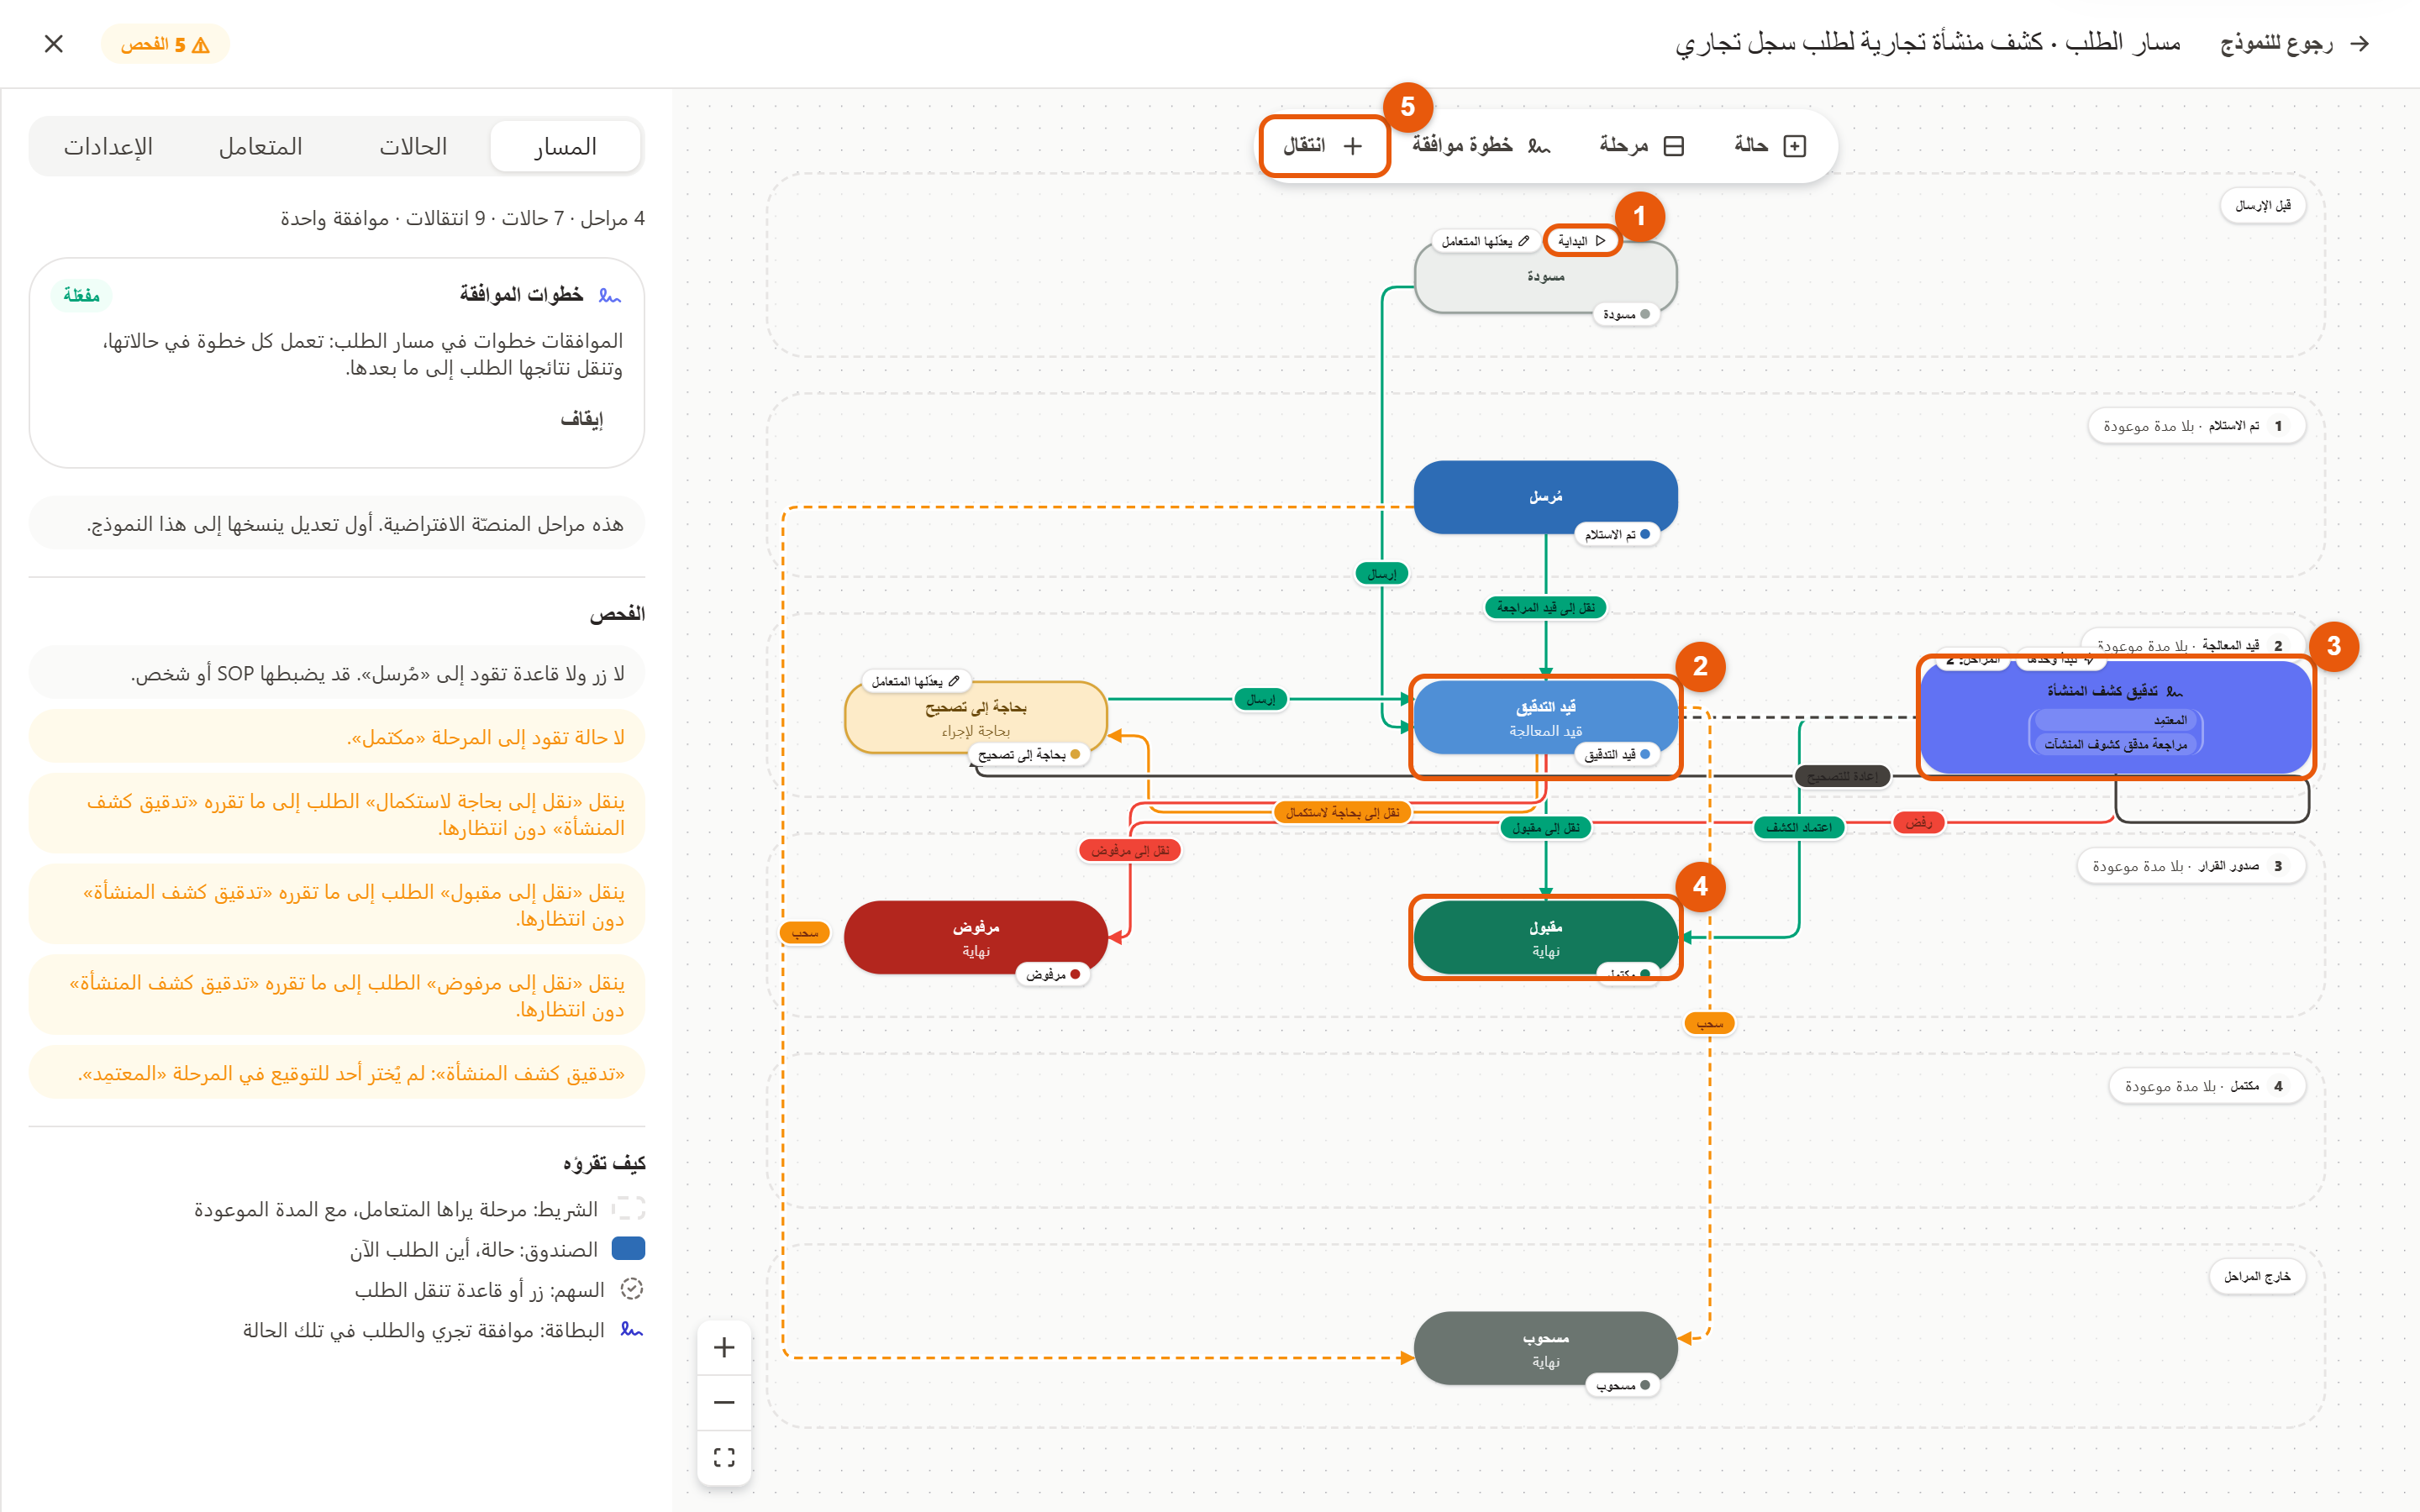
\includegraphics[width=0.95\linewidth]{assets/screens/journey-map.png}
\caption{إعداد مسار الكشف وخطوة الموافقة}
\label{fig:journey}
\shotnote{توضح الخريطة الفرق بين الحالات وخطوة القرار، وتظهر فيها ملاحظات الفحص التي يجب معالجتها قبل النشر. ① البداية. ② حالة «قيد التدقيق». ③ خطوة «تدقيق كشف المنشأة». ④ حالة «مقبول». ⑤ أداة إضافة انتقال.}
\end{figure}

\textbf{تحقق:} على الخريطة يجب أن ترى سهم «إرسال» من «مسودة» إلى «قيد التدقيق»، وبطاقة الخطوة بجانب «قيد التدقيق»، وثلاثة أسهم منها إلى «مقبول» و«مرفوض» و«بحاجة إلى تصحيح»، وسهم إرسال من «بحاجة إلى تصحيح» إلى «قيد التدقيق».

\subsection{رابعاً: اقرأ «الفحص» وأصلح كل تنبيه}

لوحة «الفحص» تقرأ المسار وتنبهك إلى ما يمنعه من العمل. عندما يكتمل المسار تظهر «لا شيء يحتاج انتباهاً». طابق التنبيهات مع الأرقام في الصورة: عالج ① بتحديد الموقّع، ثم ② بحذف أي سهم يصل إلى «مقبول» دون أن يمر بقرار ريم، ثم ③ بربط المرحلة بالحالة التي تشغّلها. أعد قراءة الفحص بعد كل تصحيح.

\begin{figure}[H]
\centering
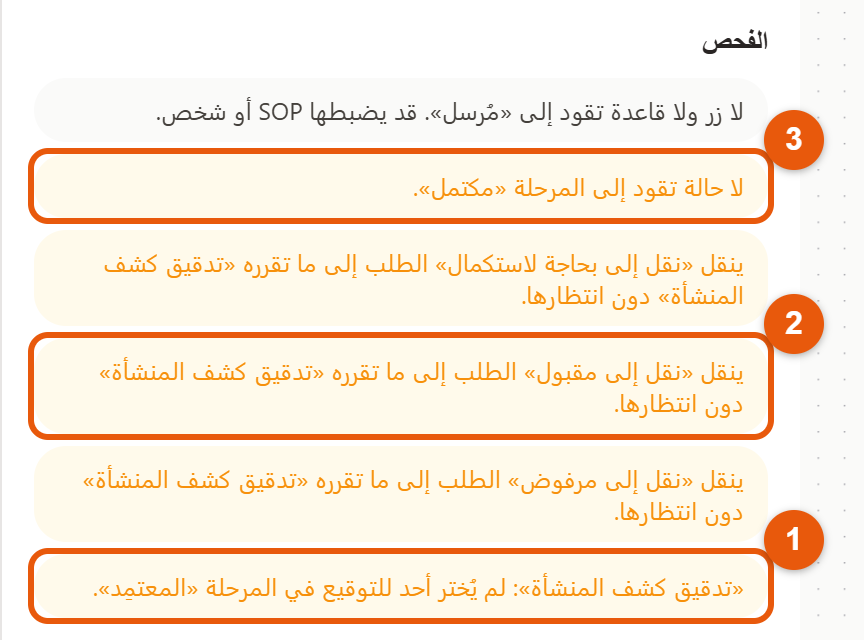
\includegraphics[width=0.8\linewidth]{assets/screens/journey-check.png}
\caption{قراءة تنبيهات فحص المسار وإصلاح أسبابها}
\label{fig:journey-check}
\shotnote{هذه شاشة تشخيص قبل اكتمال إعداد المسار. ① «لم يُختر أحد للتوقيع»: افتح المرحلة وحدد منصب المدقق. ② انتقال إلى «مقبول» دون انتظار الموافقة: احذف الزر الذي يتجاوز الخطوة، أو اجعل الانتقال من نتيجة «اعتماد الكشف» فقط. ③ لا حالة تقود إلى المرحلة: اربط المرحلة بحالة يصل إليها الكشف؛ لا تترك مرحلة لا يمكن الوصول إليها.}
\end{figure}

\begin{table}[H]
\centering
\caption{تنبيهات شائعة في «الفحص» وإصلاحها}
\label{tab:journey-warnings}
\begin{tabularx}{\linewidth}{Y Y}
\rcHeaderRow
\thh{التنبيه} & \thh{الإصلاح}\\
لم يُختر أحد للتوقيع في المرحلة «المعتمِد». & افتح المرحلة واختر المنصب في «محدد العضوية».\\
ينقل «مقبول» الطلب إلى … دون انتظار «تدقيق كشف المنشأة». & يوجد زر يتجاوز القرار. احذفه أو غيّر وجهته.\\
لا يمكن أن تعمل خطوتان في حالة واحدة. & لكل حالة خطوة موافقة واحدة. احذف الخطوة المكررة.\\
المرحلة لا يشغلها أحد، فيبقى الطلب بانتظارها دون نهاية. & المنصب المختار بلا تعيين نشط. راجع تعيين ريم.\\
لا زر ولا قاعدة تقود إلى «مُرسل». & متوقع في مثالنا لأن الإرسال يذهب إلى «قيد التدقيق» مباشرة. هذا تنبيه للعلم، لا يمنع العمل.\\
\end{tabularx}
\end{table}

\textbf{تحقق:} تستطيع أن تجيب عن أربعة أسئلة لكل سهم: ما الذي يشغّله؟ من يملك تنفيذه؟ إلى أين يصل؟ وهل يكتب في ملف المنشأة؟ لا تنشر قبل أن تفهم كل سهم.

\section{امنح الوصول وانشر النموذج}
\label{sec:build-publish}

\textbf{لماذا؟} معرفة النظام بمنصب نور لا تمنحه أي صلاحية تلقائياً. نحتاج أربعة أذونات منفصلة:

\begin{enumerate}
\item إذن على \textbf{النموذج}: كي يفتح نور الكشف ويرسله.
\item إذن على \textbf{المنشآت التجارية}: كي يرى نور قائمة المنشآت ويختار الفرن.
\item إذن \textbf{كتابة} للنموذج على المنشآت: منحناه في الخطوة السابقة.
\item \textbf{إسناد} القرار إلى ريم: ضبطناه في خطوة الموافقة.
\end{enumerate}

منح واحد منها لا يعوّض غياب الآخر. ولا يحتاج الباحث إلى أي صلاحية على أدوات البناء ليعبئ كشفاً.

\subsection{أولاً: الوصول إلى النموذج}

\begin{table}[H]
\centering
\caption{صلاحيات «الوصول» في النموذج}
\label{tab:form-access}
\begin{tabularx}{\linewidth}{R{3cm} Y}
\rcHeaderRow
\thh{الصلاحية} & \thh{معناها}\\
قائمة & رؤية الكشوف في القوائم.\\
فتح & فتح الكشف وقراءته.\\
تعديل & تعديل إجابات كشف يستطيع فتحه.\\
إرسال الطلبات & إرسال كشف يستطيع تعديله، حتى لو بدأه غيره.\\
مشاركة، حذف & مشاركة الكشف مع آخرين، أو حذفه. لا نعطيهما للفريق.\\
بدء الموافقات & بدء خطوة موافقة يدوياً. لا نحتاجها لأن خطوتنا تبدأ وحدها.\\
\end{tabularx}
\end{table}

\begin{enumerate}
\item في النموذج افتح «الوصول». تظهر ثلاث مجموعات: «من يبدأ النموذج» (موجودة دائماً)، و«أشخاص ثابتون» (أعضاء أو مناصب أو وحدات بعينها)، و«من الإجابات» (يُحددون من سؤال، مثل مدير مقدم الطلب).
\item اضغط «إضافة أشخاص ثابتين». في «الاسم» اكتب «فريق الكشف»، وفي «من» اختر منصب «باحث ميداني — 01»، وفي «يستطيع» اختر «قائمة» و«فتح» و«إرسال الطلبات»، ثم «حفظ في المسودة».
\item أضف مجموعة ثانية «المدقق ورئيس الفريق» بمنصبي «مدقق كشوف المنشآت — 01» و«رئيس فريق الكشف الميداني — 01»، مع «قائمة» و«فتح». قرار ريم لا يحتاج صلاحية «تعديل»: يصلها من خطوة الموافقة.
\end{enumerate}

\subsection{ثانياً: دور يقرأ المنشآت}

«الدور» مجموعة صلاحيات تعطيها لعدة مناصب دفعة واحدة. سننشئ دوراً واحداً يقرأ المنشآت، ونعطيه للمناصب الثلاثة.

\begin{enumerate}
\item افتح «الإعدادات» ← «الأدوار»، واضغط «إضافة الدور». تفتح نافذة «إنشاء الدور».
\item اكتب «مراقب حماية المستهلك» في «عنوان الدور». «الكود» اختياري: إذا تركته فارغاً يولّده النظام من العنوان، مثل \en{mraqb\_hmayt\_almsthlk}، ولا يتغير بعد الإنشاء. اترك «النطاق» «المنظمات»، ثم اضغط «إنشاء الدور».
\item في صفحة الدور افتح تبويب «المسؤولين»، ثم «تعيين الأعضاء والمناصب والعقد». اضغط شريحة «المناصب» واختر المناصب الثلاثة. بجانب كل منصب يظهر نطاقه: «فقط» يعني المنصب نفسه، و«الأبناء» يضيف المناصب التي تتبعه. اختر «فقط».
\item افتح «ادوات البناء» ← «الكيانات» ← «المنشآت التجارية» ← «الصلاحيات» ← «الأدوار». في صف «مراقب حماية المستهلك» فعّل «قائمة» (الرؤية في القوائم) و«فتح» (فتح سجل). لا تفعّل «تعديل» أو «حذف»: التصحيح يمر عبر الكشف المعتمد فقط.
\item اضغط «المراجعة والنشر» ثم «نشر … تغيير». الصلاحيات هنا لا تعمل قبل النشر.
\end{enumerate}

\subsection{ثالثاً: انشر النموذج}

\begin{enumerate}
\item عد إلى النموذج واضغط «اختبار النموذج». اختر منشأة، وتأكد من ظهور بياناتها والأسئلة المطلوبة.
\item اضغط «نشر». إذا ظهرت «يرجى إصلاح الخطأ قبل نشر النموذج» فعالج الخطأ المذكور أولاً.
\item تفتح نافذة «نشر الإصدار 1» وتحتها «نشر أول: كل شيء جديد». اقرأ قائمة التغييرات، واكتب في «ملاحظة التغيير (اختيارية)» جملة مثل «الإصدار الأول لكشف المنشآت»، ثم اضغط «نشر».
\item تظهر «تم نشر النموذج بنجاح».
\end{enumerate}

\begin{figure}[H]
\centering
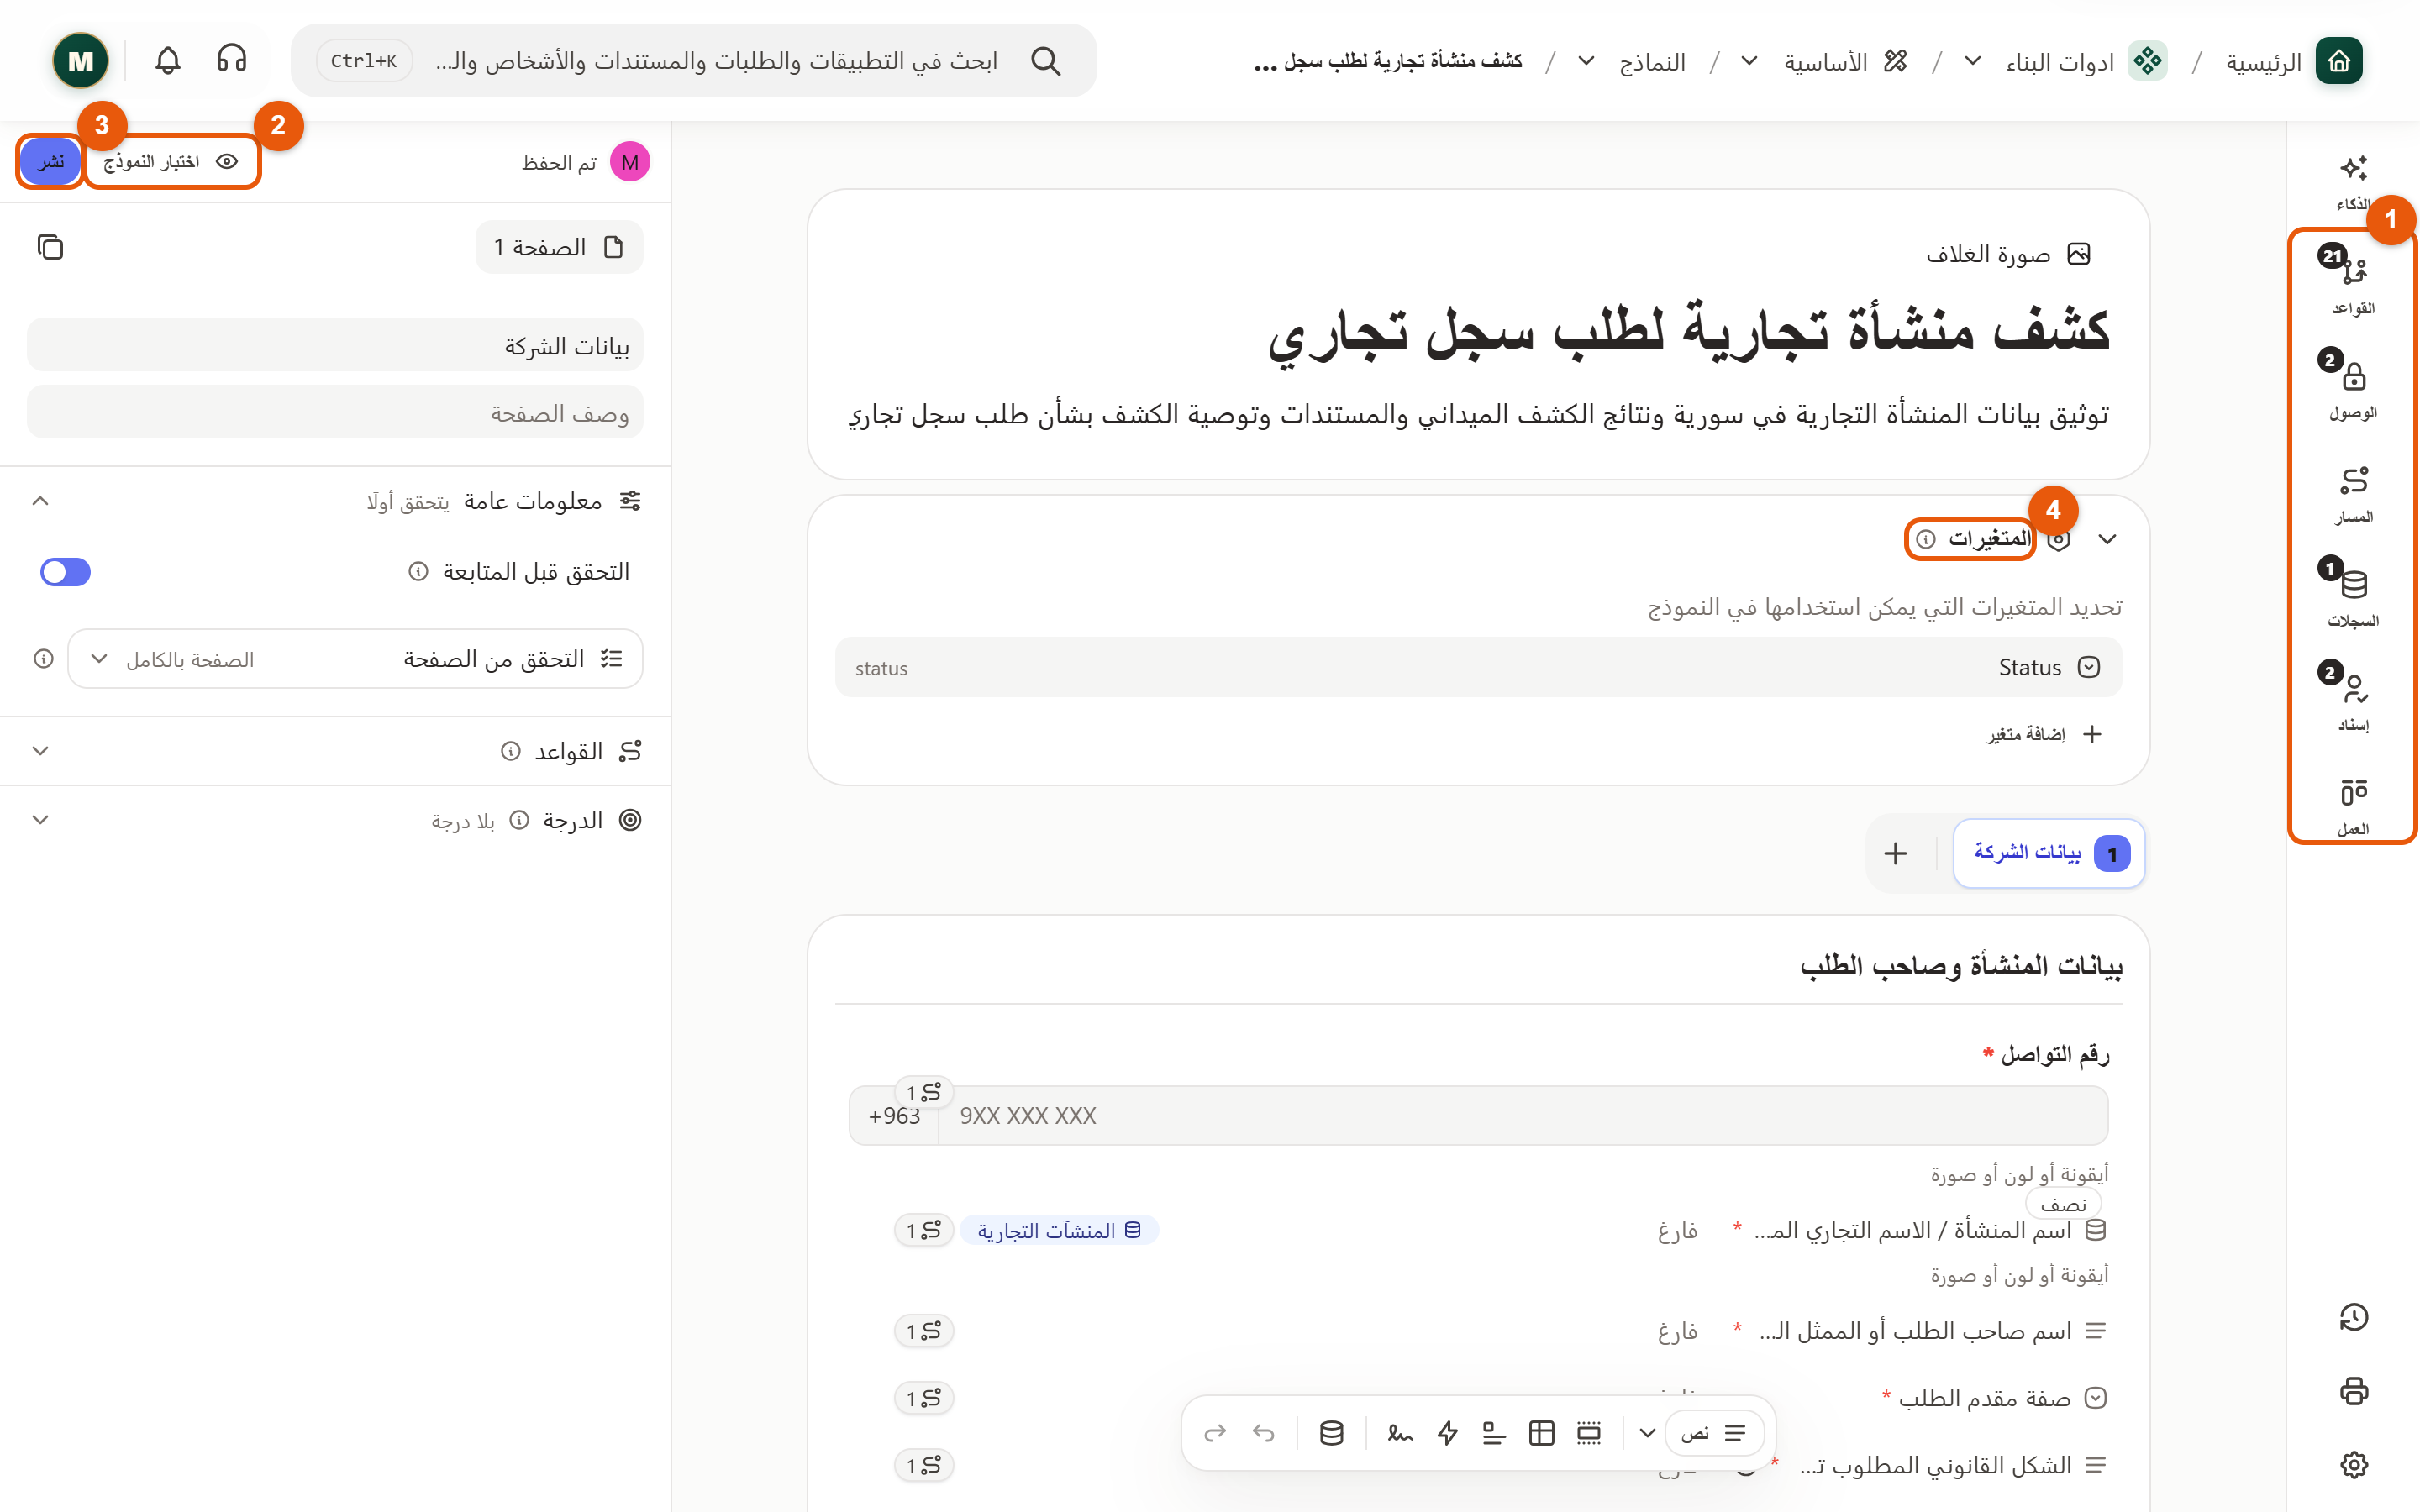
\includegraphics[width=0.95\linewidth]{assets/screens/form-builder.png}
\caption{أدوات الإعداد والاختبار والنشر}
\label{fig:builder}
\shotnote{الشريط الجانبي يجمع الإعدادات التي أكملتها، بينما يبقى الاختبار والنشر أعلى المحرر. ① أدوات الربط والوصول والمسار والتكليف. ② «اختبار النموذج»: جرّب الأسئلة قبل التشغيل. ③ «نشر»: أتح النسخة للفريق. ④ «المتغيرات»: قيم يستخدمها النموذج، ولا تحتاج لإضافة متغير جديد لمجرد ربط المنشأة.}
\end{figure}

\begin{rcnote}[ماذا يحدث للكشوف عند نشر إصدار جديد؟]
الكشف الذي بدأه نور يبقى على الإصدار الذي بدأ به، والكشوف الجديدة تستخدم الإصدار الجديد. وتعديل النموذج بعد النشر يبدأ مسودة جديدة؛ يبقى الإصدار المنشور يعمل حتى تنشر المسودة. تجد كل الإصدارات في «الإصدارات».
\end{rcnote}

\textbf{تحقق:} يستطيع الباحث فتح النموذج وقراءة المنشأة. إذا ظهر منع وصول، افحص صلاحية النموذج وصلاحية «المنشآت التجارية» كلّاً على حدة.

\subsection{افصل الصلاحيات حتى تعرف سبب كل منع}

إذا لم يستطع نور فتح الاستمارة فالمشكلة في «الوصول». وإذا فتحها ولم يجد الفرن فالمشكلة في صلاحيات «المنشآت التجارية». وإذا اعتُمد الكشف ولم يتغير الملف فالمشكلة في إذن الكتابة. وإذا لم يصل الكشف إلى ريم فالمشكلة في «من يوقّع» أو في تعيينها. كل عرض له مكان واحد تبحث فيه.

\subsection{اختبر النسخة قبل تكليف الفريق}

«اختبار النموذج» يشغّل المسودة في جلسة معزولة: لا يتحول شيء فيها إلى كشف حقيقي، ولا تُكتب في أي سجل، ولا تُرسل إشعارات. تستطيع في «الاختبار بصفة» أن تختار «عضو» وتجرّب بصلاحيات نور الحقيقية. أما وصول الموافقة إلى ريم وكتابة التصحيح في الملف، فتختبرهما بكشف فعلي في الخطوات التالية.

\begin{table}[H]
\centering
\caption{اختبارات النموذج ونتائجها المطلوبة}
\label{tab:form-acceptance}
\begin{tabularx}{\linewidth}{Y Y}
\rcHeaderRow
\thh{التجربة} & \thh{النتيجة التي تبحث عنها}\\
الإرسال دون منشأة أو توصية & تظهر «أجب عن الأسئلة المطلوبة» ويُمنع الإرسال.\\
اختيار الفرن & تمتلئ الحقول المرتبطة من ملفه.\\
التوصية بعدم الموافقة دون أسباب & تعمل قاعدة الإلزام، ثم يُسمح بالإرسال بعد كتابة السبب.\\
تصحيح العنوان ثم إرسال الكشف & يبقى عنوان الملف القديم إلى حين الاعتماد.\\
إعادة الكشف من ريم إلى نور & يصل التعليق لنور ويستطيع التصحيح وإعادة الإرسال.\\
رفض كشف & لا يُكتب شيء في الملف.\\
اعتماد كشف & يصبح «مقبول»، ويتغير ملف الفرن.\\
فتح النموذج بحساب الباحث & تعمل صلاحياته دون الاعتماد على صلاحيات المسؤول الذي بناه.\\
\end{tabularx}
\end{table}

\textbf{تحقق:} لا تعتبر النموذج جاهزاً لمجرد أن نشره نجح. الجاهزية تعني أن الباحث يستطيع تعبئته، والمدقق يستطيع اتخاذ القرارات الثلاثة، والكتابة تحدث في موعدها وعلى الملف الصحيح.

\section{كلّف الباحث بالكشف على المنشأة}
\label{sec:build-plan}

\textbf{لماذا؟} النموذج يحدد \textbf{ما} سيُعبأ. أما التكليف فيحدد \textbf{من} سيعبئه، وعن \textbf{أي منشأة}، و\textbf{متى}. سنطلب من نور تعبئة كشف عن فرن الأمانة. نفعل ذلك في مكانين: إعداد التكليف في النموذج، ثم «خطة تكليف» توزع العمل.

\subsection{أولاً: اسمح بالتكليف في النموذج}

افتح النموذج واضغط «إسناد» في الشريط الجانبي. تفتح لوحة «التكليف». يجب أن يكون النموذج منشوراً قبل هذا.

\begin{figure}[H]
\centering
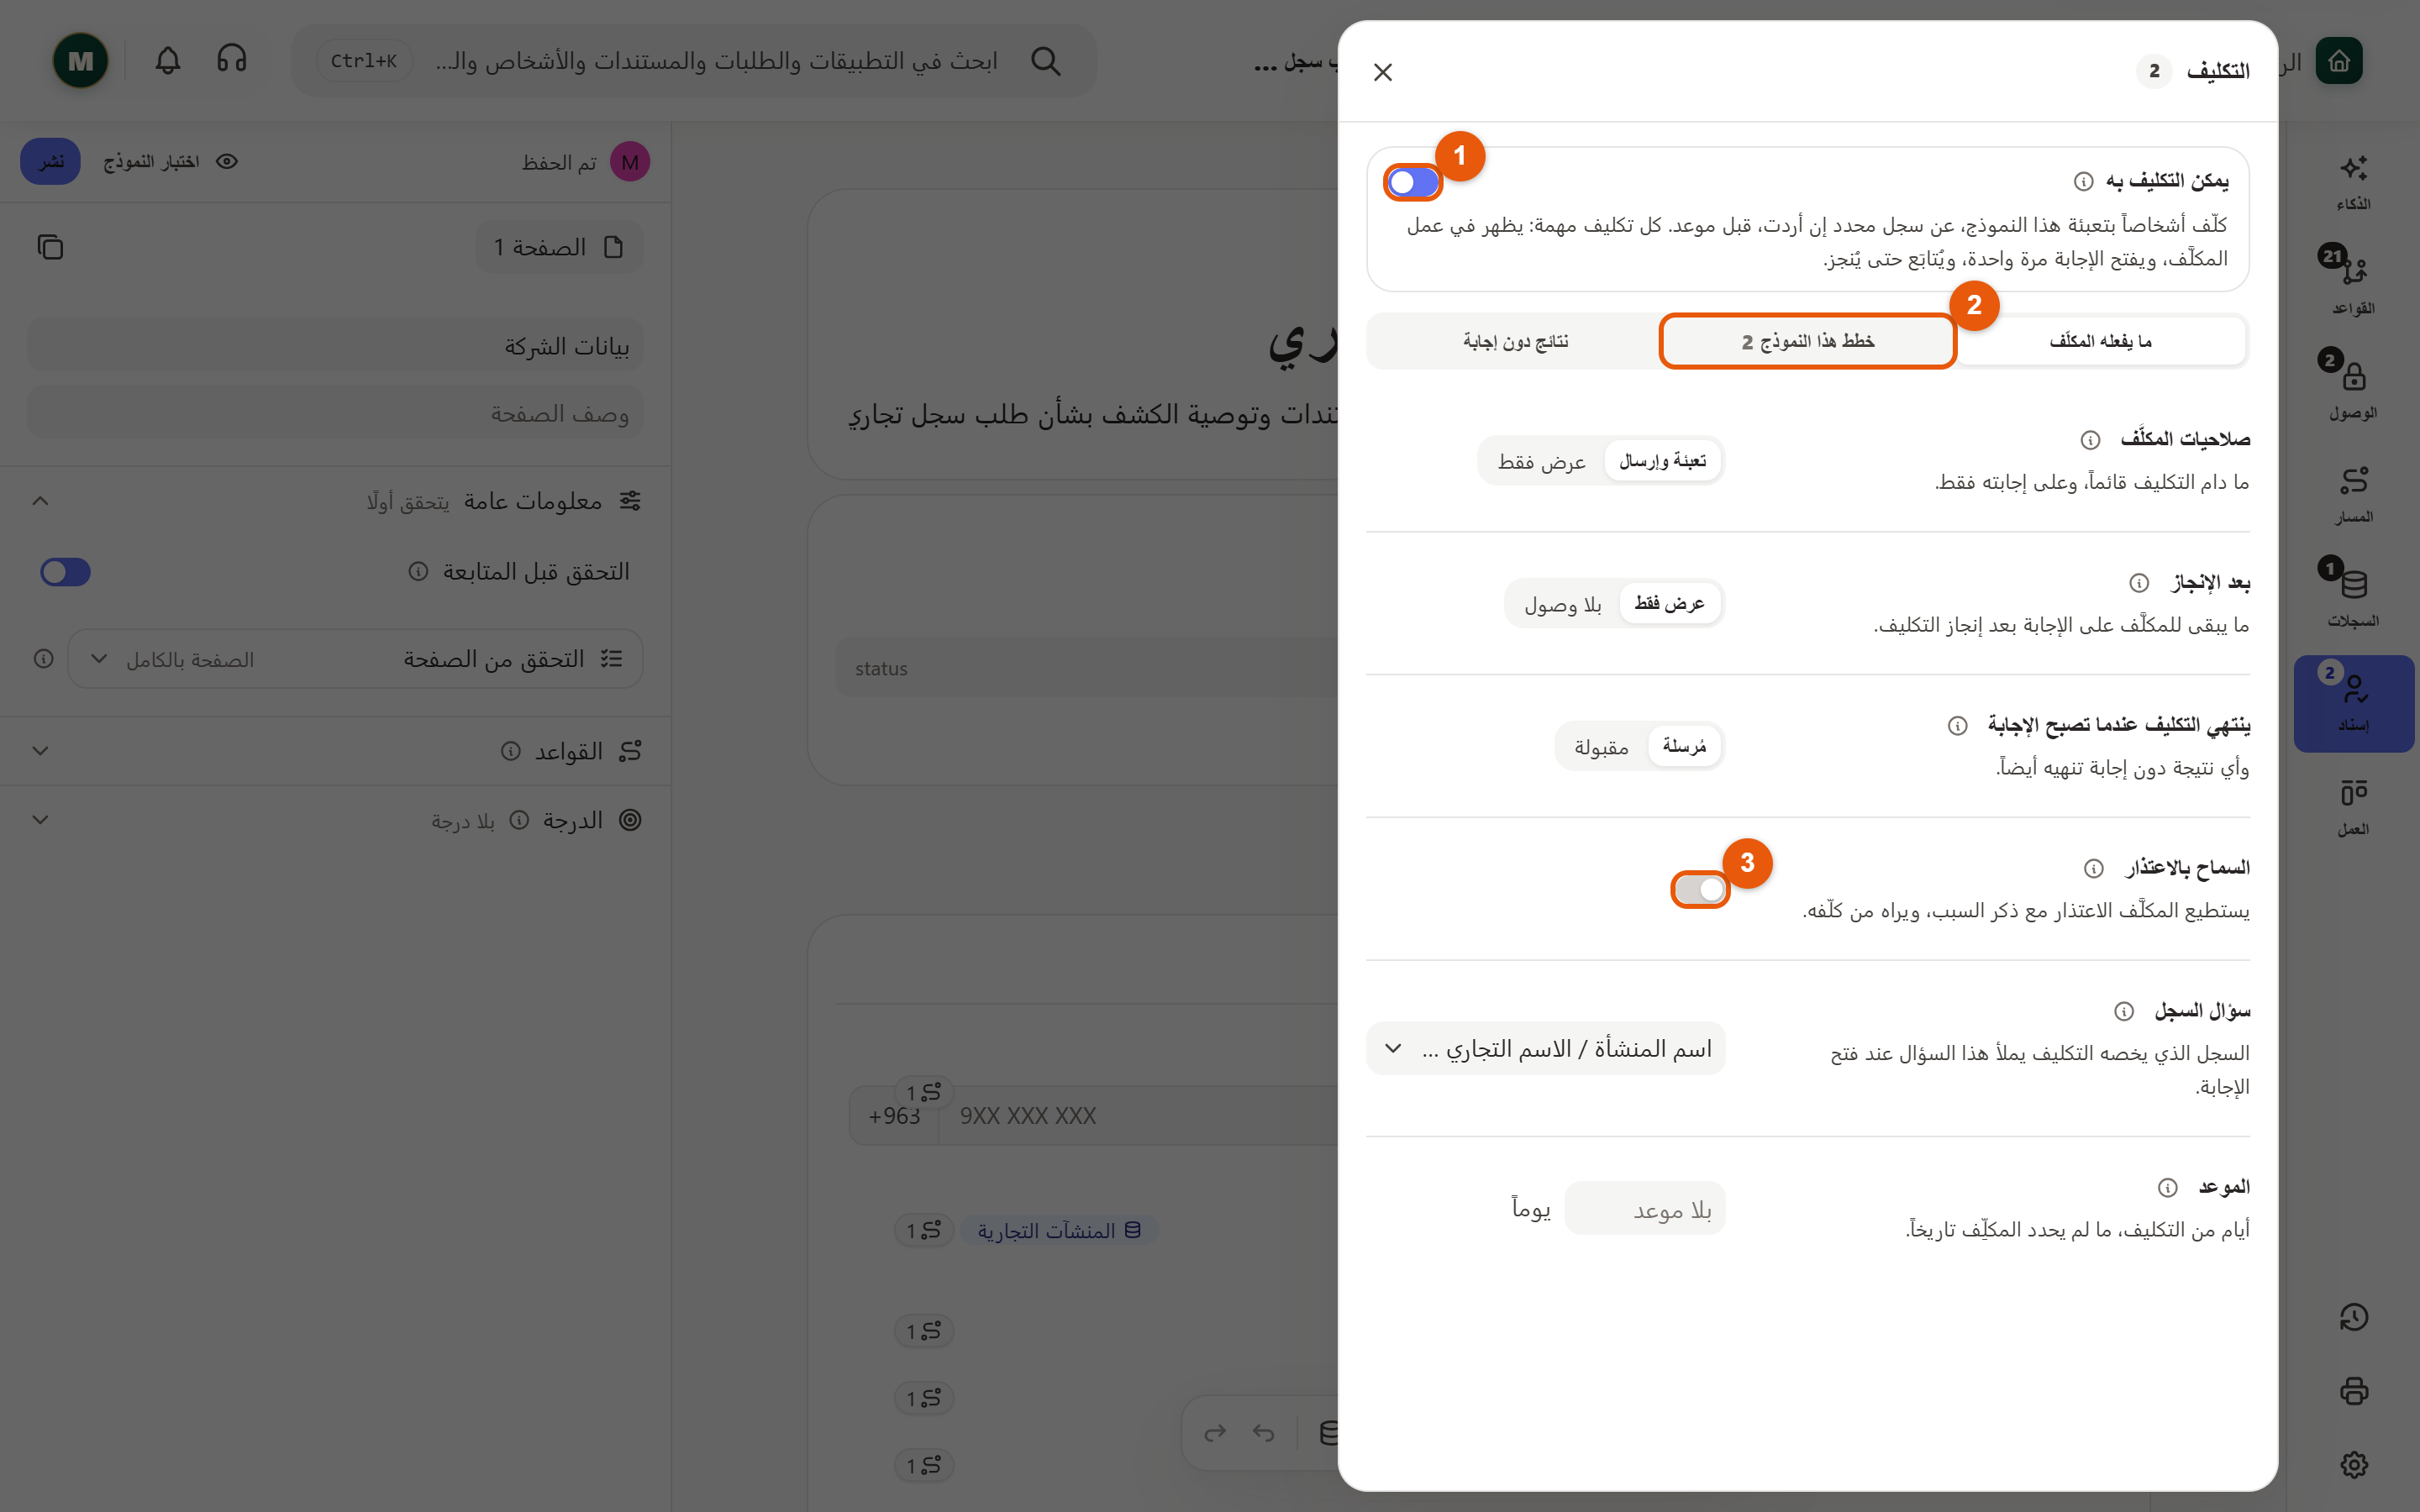
\includegraphics[width=0.95\linewidth]{assets/screens/form-assign.png}
\caption{السماح بتكليف شخص بتعبئة النموذج}
\label{fig:assign}
\shotnote{تحدد هذه الشاشة كيف يعمل التكليف، وما يمكن للباحث فعله في إجابته. ① «يمكن التكليف به»: متوقف افتراضياً، وما دام متوقفاً لا يمكن لأحد التكليف بالنموذج. ② «خطط هذا النموذج»: افتح الخطط المرتبطة به. ③ «السماح بالاعتذار»: خيار إضافي إن كانت إجراءات العمل تسمح باعتذار الباحث.}
\end{figure}

\begin{table}[H]
\centering
\caption{إعدادات «ما يفعله المكلّف»}
\label{tab:assign-settings}
\begin{tabularx}{\linewidth}{R{3.4cm} Y Y}
\rcHeaderRow
\thh{الإعداد} & \thh{الخيارات} & \thh{اختيارنا ولماذا}\\
صلاحيات المكلَّف & «تعبئة وإرسال» أو «عرض فقط». & «تعبئة وإرسال»: نور يملأ الكشف ويرسله. هذه الصلاحية على إجابته فقط وما دام التكليف قائماً.\\
بعد الإنجاز & «عرض فقط» أو «بلا وصول». & «عرض فقط»: يرى نور كشفه بعد إنجازه.\\
ينتهي التكليف عندما تصبح الإجابة & «مُرسلة» أو «مقبولة». & «مقبولة»: تبقى المهمة مفتوحة عند نور حتى تعتمد ريم، فإذا أعادته للتصحيح يجده في مهامه.\\
السماح بالاعتذار & مفعّل أو متوقف. & متوقف، إلا إذا كانت إجراءاتكم تسمح للباحث بالاعتذار مع ذكر السبب.\\
سؤال السجل & أسئلة السجل في النموذج. & «اسم المنشأة / الاسم التجاري المقترح»: يفتح التكليف والفرن مختار مسبقاً.\\
الموعد & عدد أيام، أو «بلا موعد». & مثلاً 7 أيام من التكليف.\\
\end{tabularx}
\end{table}

\begin{enumerate}
\item فعّل «يمكن التكليف به» عند ①.
\item اضبط الإعدادات كما في الجدول، ثم اضغط «حفظ».
\end{enumerate}

\subsection{ثانياً: أنشئ خطة التكليف}

\begin{enumerate}
\item افتح «خطط التكليف» ← «خطة جديدة». تفتح نافذة «خطة تكليف جديدة».
\item في «ماذا سيعبّئ الأشخاص؟» اختر «كشف منشأة تجارية لطلب سجل تجاري»؛ يجب أن تظهر بجانبه شارة «جاهز». (إذا ظهرت «التكليف متوقف لهذا النموذج» فارجع وفعّل «يمكن التكليف به».) اكتب في «اسم الخطة» «جولة كشف فرن الأمانة»، ثم اضغط «إنشاء والإعداد».
\item تفتح الخطة في أقسام مرقمة. اضبطها كما في الجدول التالي. القسم الذي فيه مشكلة يعرض سببها، مثل «اختر نوع السجل.» أو «أضف مرشحين.».
\end{enumerate}

\begin{table}[H]
\centering
\caption{أقسام خطة التكليف}
\label{tab:plan-sections}
\begin{tabularx}{\linewidth}{R{3cm} Y Y}
\rcHeaderRow
\thh{القسم} & \thh{ما فيه} & \thh{اختيارنا}\\
1 · السجلات & «نوع السجل»، و«متى تُنشأ التكليفات»، و«السجلات». & «المنشآت التجارية»؛ «عند الإطلاق»؛ «اختيار سجلات» ثم «فرن الأمانة». (الخيار الآخر «كل السجلات المطابقة» يكلّف بكل منشأة تطابق شرطاً.)\\
2 · المرشحون & «المرشحون من»: «حقل في السجل» أو «قائمة ثابتة» أو «سجلات تشير إليه» أو «بالكود». & «قائمة ثابتة» ثم منصب «باحث ميداني — 01». «حقل في السجل» مفيد لاحقاً إذا كان لكل منشأة باحث مسؤول عنها.\\
3 · التوزيع بين المرشحين & «يُكلَّف»: «شخص واحد» أو «كلهم · إجابة مشتركة» أو «قائمة يستلمون منها». & «شخص واحد».\\
4 · المراجعون & من يراجع الكشوف. & اتركه كما في النموذج: ريم من خطوة الموافقة.\\
5 · الموعد والتذكير & الموعد، و«ينتهي التكليف عندما تصبح الإجابة»، و«الاعتذار». & يظهر بجانب كل منها «من النموذج»: اتركها تأخذ إعداد النموذج.\\
6 و7 ومتقدم & المتابعة، ومن يدير الخطة، وإصدار النموذج. & اتركها كما هي.\\
\end{tabularx}
\end{table}

بعد ضبط الأقسام:

\begin{enumerate}
\item اضغط «تشغيل المعاينة». يظهر سطر مثل «المعاينة: 1 سجلات ← 1 تكليفات لـ1 أشخاص». افتح التفاصيل وتأكد أن «فرن الأمانة» يقابل «نور حسن — تجريبي».
\item اضغط «حفظ»، ثم «إنشاء التكليفات». تسأل النافذة «إنشاء التكليفات الآن؟ تصل الإشعارات إلى المكلَّفين فوراً.»؛ أكّد.
\end{enumerate}

\begin{figure}[H]
\centering
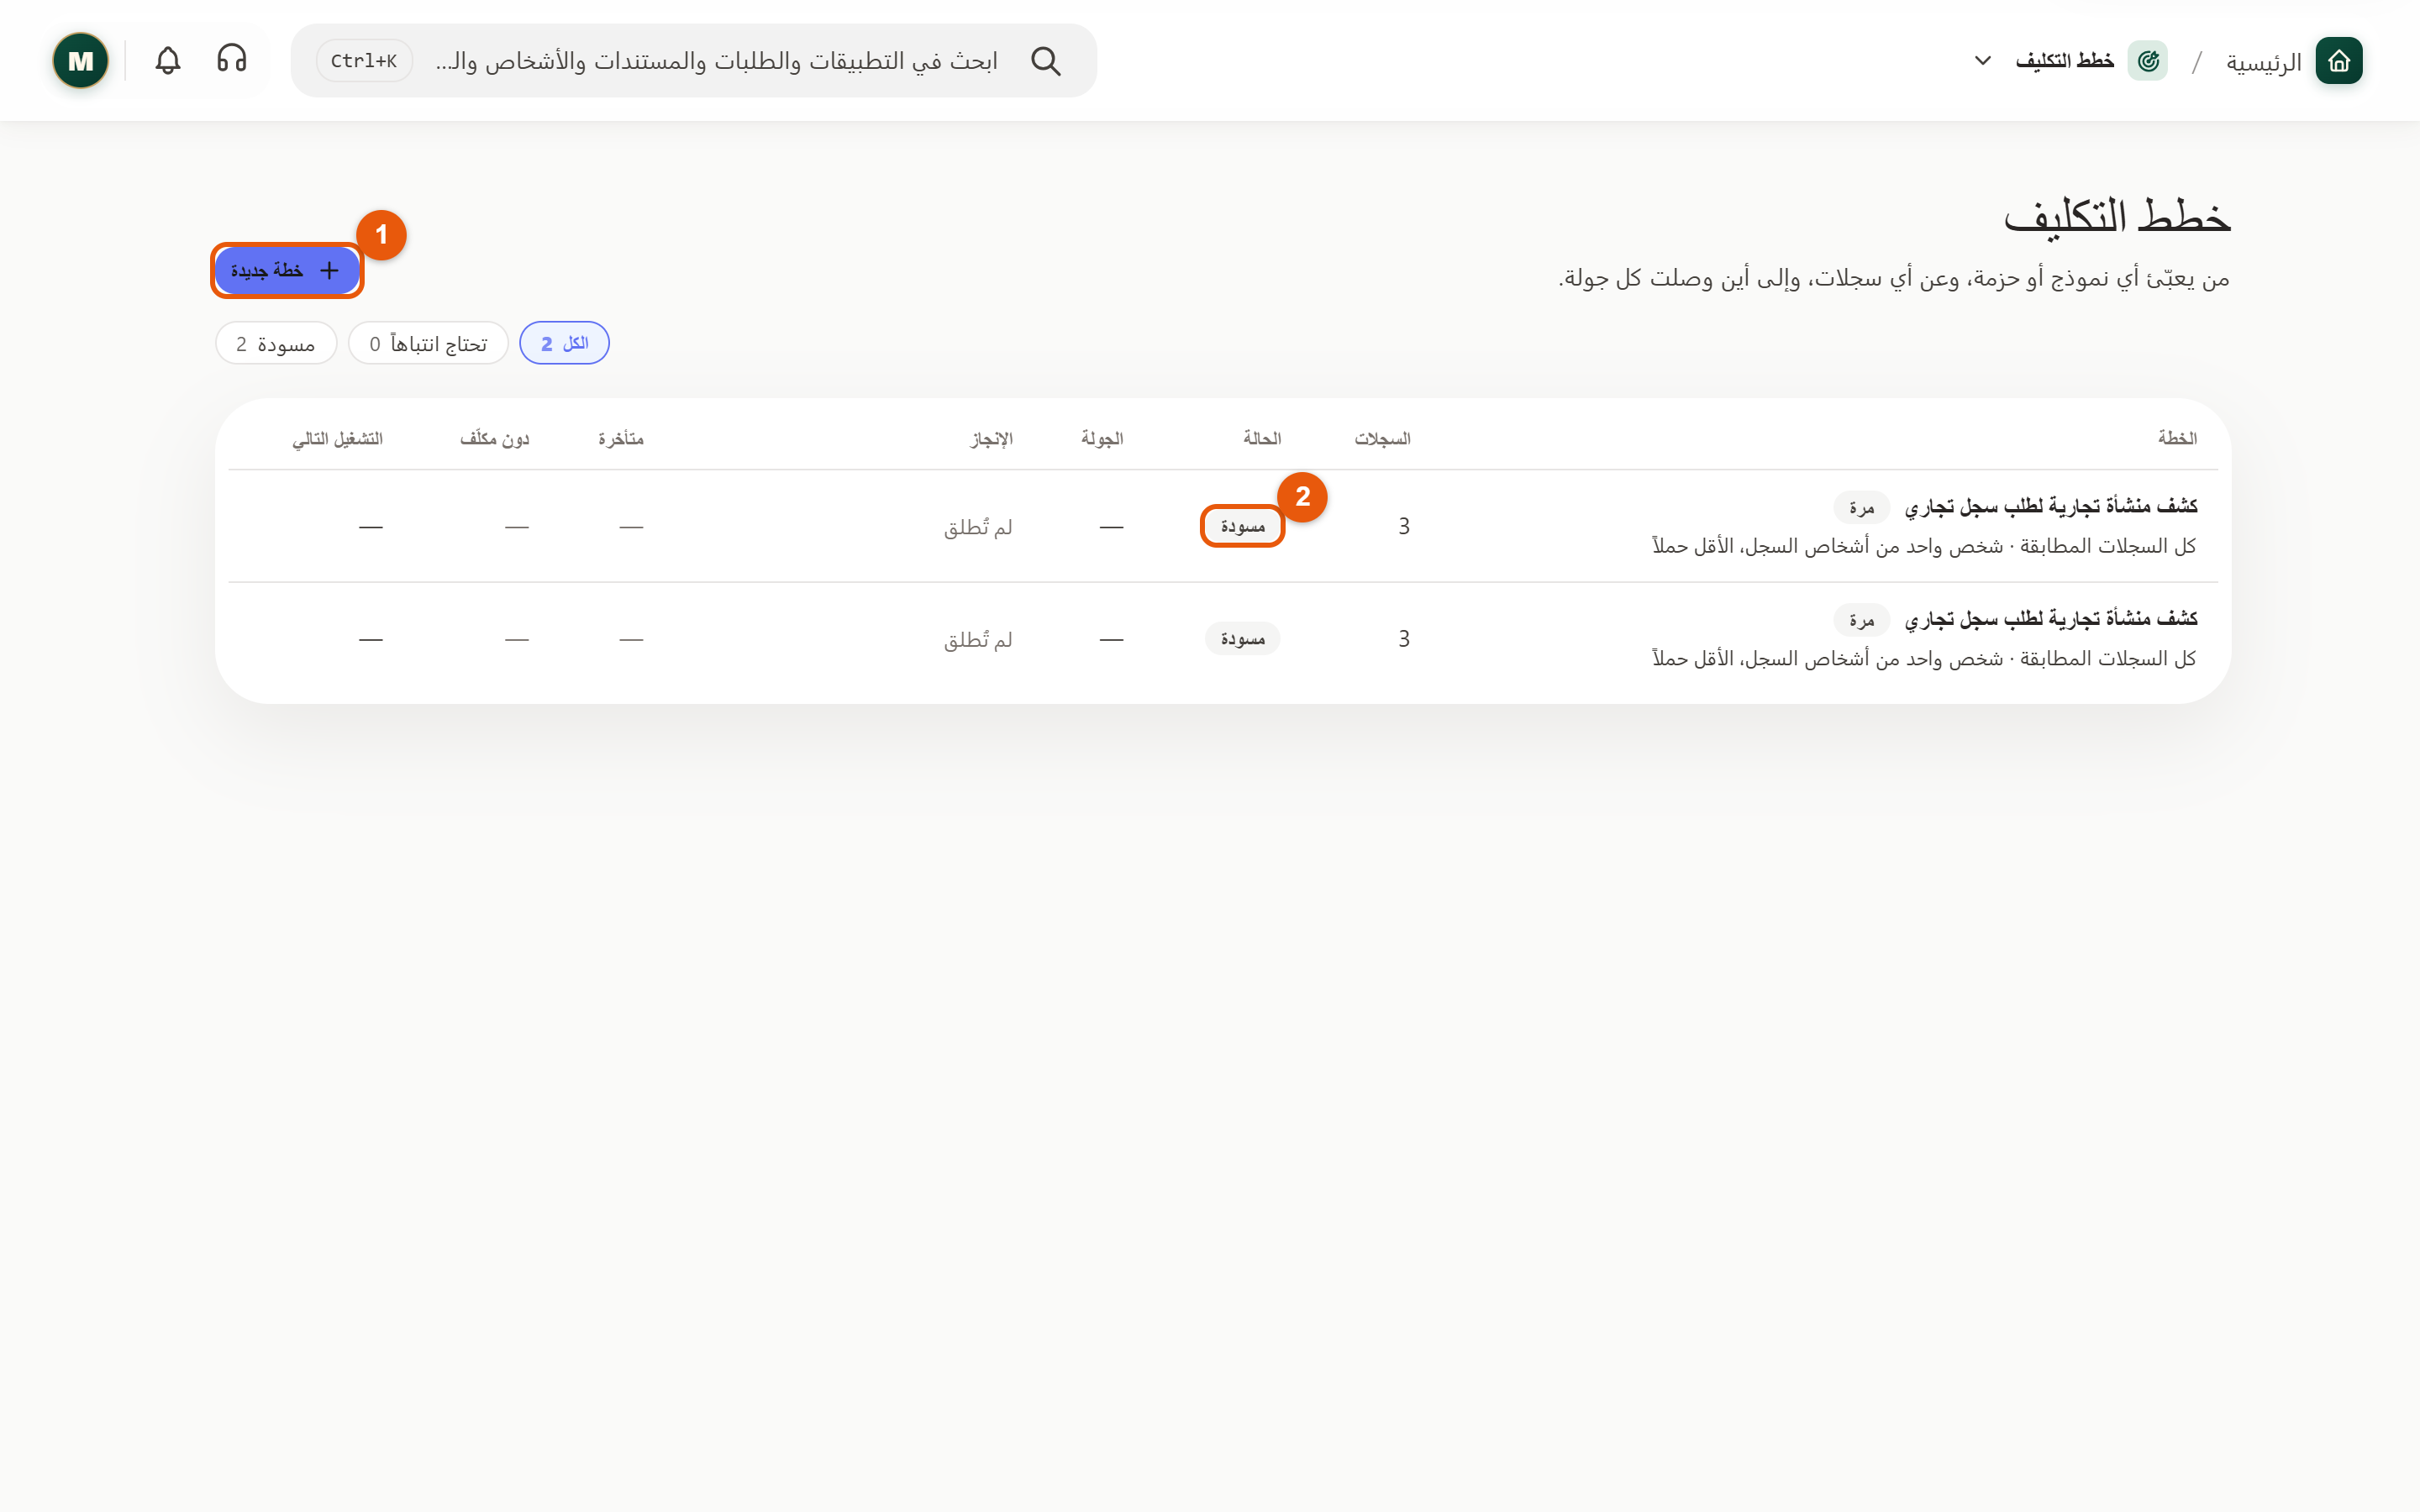
\includegraphics[width=0.95\linewidth]{assets/screens/plans-list.png}
\caption{من مسودة خطة إلى تكليف فعلي}
\label{fig:plans}
\shotnote{الخطة المحفوظة كمسودة لا تعني أن العمل وصل إلى الباحث. ① «خطة جديدة»: ابدأ إعداد الجولة. ② «مسودة»: أكمل الإعداد والمعاينة ثم اضغط «إنشاء التكليفات» لإطلاق العمل؛ بعدها تصبح الخطة «نشطة».}
\end{figure}

\textbf{تحقق:} تصبح حالة الخطة «نشطة» بدل «مسودة»، ويظهر التكليف لنور في «تكليفات مطلوبة منك». إذا عرضت المعاينة «دون مرشح» فاقرأ السبب بجانبه: «لا شاغل للمنصب هناك» يعني أن تعيين نور غير نشط أو غير موجود.

\section{نفّذ الكشف وأرسله للتدقيق}
\label{sec:build-run}

\textbf{ماذا يفعل الباحث؟} يفتح نور المهمة، ويتأكد من المنشأة، ثم يسجل ما وجده في الزيارة. تحفظ الإجابة تفاصيل الزيارة، أما تعديل ملف المنشأة فينتظر قرار ريم.

\begin{enumerate}
\item يدخل نور بحسابه. في الصفحة الرئيسية يجد بطاقة «تكليفات مطلوبة منك»، وفيها الكشف عن فرن الأمانة وموعده. يضغط «ابدأ».
\item يرى الفرن مختاراً في سؤال المنشأة، ومحافظته وعنوانه ونشاطه وموقعه معبأة، وبجانبها «من السجل».
\item إذا وجد العنوان تغيّر، يصححه. تظهر بجانب السؤال «تغيّر» مع القيمة القديمة بعد «كانت»، ويستطيع إلغاء تصحيحه بـ«استعادة».
\item يكتب «ملاحظات الكشف»، ويختار التوصية، ويكتب الأسباب إن طُلبت، ويرفع الصور.
\item يضغط «إرسال الطلب». تسأل النافذة «إرسال الطلب؟» وتنبه «لن تتمكّن من تعديله أثناء معالجته.». يضغط «إرسال الطلب» مرة ثانية.
\item إذا ظهرت «أكمل الحقول المطلوبة قبل الإرسال.» أو «للإرسال: أجب عن الأسئلة المطلوبة»، يضغط على السؤال المذكور، ويكمله، ثم يعيد الإرسال.
\end{enumerate}

\textbf{تحقق:} يتحول الكشف إلى «قيد التدقيق»، وتصل الموافقة إلى ريم. ملف الفرن يبقى بعنوانه القديم حتى الاعتماد؛ تغيير الإجابة وحده لا يغيّر الملف.

\section{اتخذ القرار وتأكد من النتيجة}
\label{sec:build-decision}

\textbf{ماذا تفعل المدققة؟} تقرأ ريم الإجابة والمرفقات، ثم تختار قراراً. الإعادة تسمح لنور بالتصحيح، والرفض ينهي الكشف دون اعتماد، والاعتماد يقبل الكشف ويكتب التصحيحات في ملف المنشأة.

\begin{enumerate}
\item تدخل ريم بحسابها، وتفتح من الصفحة الرئيسية بطاقة «موافقات بانتظارك»، ثم الكشف الخاص بفرن الأمانة.
\item تقرأ الأقسام وتفتح المرفقات. قبل القرار يظهر لها «ما سيُنشأ أو يتغيّر في السجلات»، مثل «سيتحدّث: فرن الأمانة» مع الحقول التي ستتغير.
\item في «ردك» تختار نتيجة واحدة: «اعتماد الكشف» أو «رفض» أو «إعادة للتصحيح».
\item تكتب في «التعليق (مطلوب)» سبب الرفض أو المطلوب استكماله. ثم تضغط زر التأكيد، واسمه يتبع النتيجة، مثل «تأكيد اعتماد الكشف». (إذا كانت النتيجة تحتاج توقيعاً يصبح «توقيع و…» ويطلب «الرقم السري».)
\item تظهر «تم تسجيل الرد».
\item عند الإعادة: يجد نور الكشف نفسه في مهامه بحالة «بحاجة إلى تصحيح»، ومعه تعليق ريم. يصححه ويرسله مجدداً، فتبدأ جولة تدقيق جديدة. لا ينشئ كشفاً جديداً.
\item عند الاعتماد: افتح ملف فرن الأمانة وتأكد من وصول العنوان المصحح.
\end{enumerate}

\textbf{تحقق:} اكتمل الكشف عندما أصبحت حالته «مقبول»، ووصلت التغييرات إلى ملف المنشأة. في الكشف زر «السجلات · …» يعرض نتيجة الكتابة: «كُتبت» أو «كُتبت جزئياً» أو «لم تُكتب».

\begin{rcwarn}[إذا ظهر «لم تُحفظ الإجابات في السجلات»]
قرار ريم سُجّل، لكن الكتابة في ملف المنشأة فشلت. اضغط «السجلات · لم تُحفظ» واقرأ ما بعد «السبب:». «غير مسموح» يعني أن إذن الكتابة ناقص: راجع «مسموح · 4 حقول». و«قيم غير صالحة» يعني أن القيمة لا تناسب الحقل، مثل خيار محافظة غير موجود في الحقل. و«السجل غير موجود» يعني أن ملف المنشأة حُذف. عالج السبب، ثم اضغط «اكتب مجدداً». القرار لا يتغير؛ ما يُعاد هو الكتابة فقط.
\end{rcwarn}

\section{أنشئ لوحة مؤشرات المنشآت التجارية}
\label{sec:build-dashboard}

\textbf{لماذا؟} يحتاج أحمد إلى معرفة عدد المنشآت، وأين تقع، وما أنشطتها، ثم الوصول إلى منشأة محددة. «لوحة المعلومات» تجمع هذه الإجابات في شاشة واحدة. ستقرأ اللوحة ملفات «المنشآت التجارية» مباشرة، فلا نكتب بيانات الفرن مرة أخرى؛ وكل تصحيح يُعتمد في كشف يظهر فيها.

\begin{enumerate}
\item افتح «ادوات البناء» ← «لوحات المعلومات»، واضغط «إنشاء لوحة معلومات».
\item اكتب في «اسم لوحة المعلومات» «مؤشرات المنشآت التجارية». هذا الحقل مطلوب.
\item اكتب في «الوصف» «متابعة المنشآت حسب المحافظة والنشاط والبحث عن منشأة». الوصف مطلوب، 12 حرفاً وكلمتان على الأقل.
\item اضغط «إنشاء». تظهر «تم إنشاء لوحة المعلومات بنجاح» ويفتح المحرر.
\end{enumerate}

توضح الصورة حقول البداية: اكتب الاسم عند ① والوصف عند ②، ثم اضغط «إنشاء» عند ③. الوصف يشرح غرض اللوحة، ولا يحدد مصدر بياناتها؛ المصدر تضبطه داخل كل عنصر.

\begin{figure}[H]
\centering
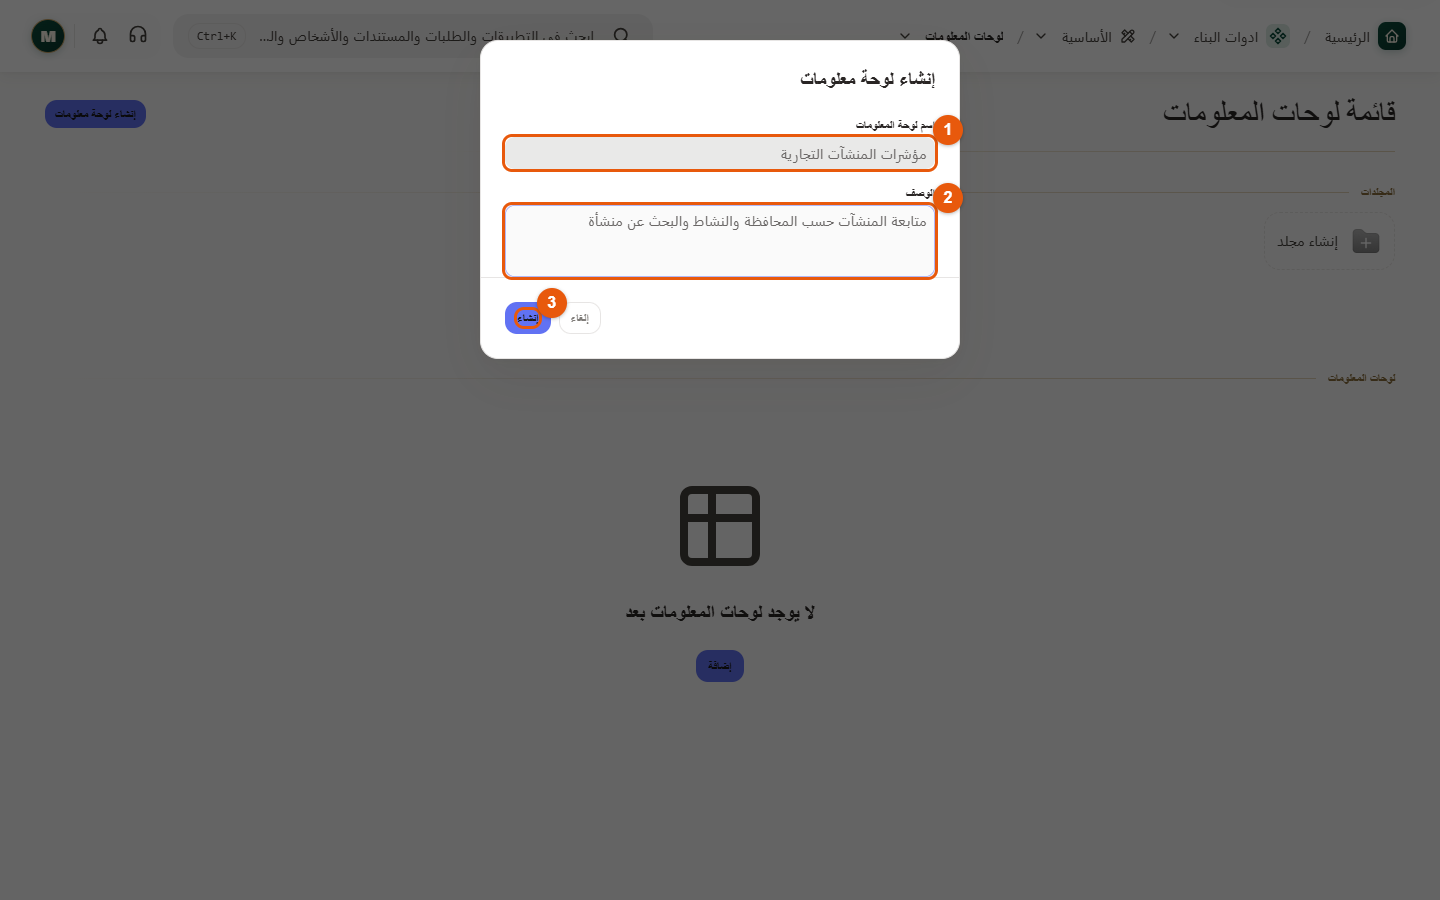
\includegraphics[width=0.95\linewidth]{assets/screens/org-dashboard-create.png}
\caption{إنشاء لوحة مؤشرات المنشآت التجارية}
\label{fig:dashboard-create}
\shotnote{① اسم اللوحة الذي سيظهر للفريق. ② وصف قصير لما سيجده المشاهد. ③ إنشاء اللوحة وفتح محررها. هذه شاشة إدخال قبل الإنشاء، وليست لوحة منشورة.}
\end{figure}

\subsection{تعرّف على المحرر}

\begin{itemize}
\item \textbf{الأزرار أعلى المحرر} أيقونات، يظهر اسم كل منها عند الوقوف عليه: «إدارة الوصول» (القفل)، و«المرشحات» (القمع)، و«الإعدادات» (الترس)، و«الإصدارات» (الساعة)، و«معاينة» (العين)، ثم «حفظ» و«نشر».
\item \textbf{شريط العناصر أسفل الشاشة} أيقونات أيضاً. نحتاج منها: «مؤشر أداء» (رقم كبير)، و«إضافة رسم بياني (Nivo)»، و«جدول».
\item \textbf{إعدادات العنصر:} اضغط على أي عنصر لتفتح لوحته بثلاثة تبويبات: «عام» (العنوان والعرض والارتفاع)، و«البيانات» (من أين يقرأ وكيف يحسب)، و«النمط» (الشكل والألوان).
\end{itemize}

\textbf{تحقق:} يظهر اسم اللوحة في المحرر. إنشاء اللوحة لا يجلب بيانات وحده؛ سنحدد مصدر كل عنصر في الخطوات التالية.

\subsection{خطط للوحة قبل إضافة عناصرها}

\begin{table}[H]
\centering
\caption{السؤال الذي يجيب عنه كل عنصر}
\label{tab:dashboard-design}
\begin{tabularx}{\linewidth}{Y Y Y}
\rcHeaderRow
\thh{سؤال أحمد} & \thh{العنصر المناسب} & \thh{الإعداد الذي يجيب عنه}\\
كم منشأة تطابق اختياراتي؟ & «مؤشر أداء» بعنوان «عدد المنشآت». & المصدر «المنشآت التجارية»، و«التجميع» «العدد».\\
كيف تتوزع حسب المحافظة؟ & رسم «أعمدة». & «حقل الفئة»: المحافظة؛ «نوع القيمة»: «عدد».\\
ما الأنشطة التي تغطيها؟ & رسم ثانٍ. & «حقل الفئة»: النشاط؛ «نوع القيمة»: «عدد».\\
ما أسماء هذه المنشآت وبياناتها؟ & «جدول». & المصدر نفسه، مع حقول الاسم والنشاط والمحافظة والعنوان.\\
كيف أصل إلى منشأة محددة؟ & مرشح من نوع «محدد». & يختار أحمد منشأة، فتتصفى العناصر بمعرّفها.\\
\end{tabularx}
\end{table}

كل صف في مصدرنا منشأة واحدة. لذلك المؤشر يعدّ المنشآت، لا الزيارات: كشفان على الفرن لا يجعلانه منشأتين. لو أردت عدّ الكشوف لاحقاً فاختر مصدراً آخر هو إجابات النموذج؛ تغيير العنوان إلى «الكشوف» لا يغيّر ما يعدّه.

\section{اربط مؤشر العدد بالمنشآت}
\label{sec:build-kpi}

\textbf{ما معنى مؤشر أداء؟} رقم كبير يجيب عن سؤال واحد. سؤالنا: كم منشأة لدينا؟ مصدر الرقم «المنشآت التجارية»، و«التجميع» هو طريقة الحساب.

\begin{enumerate}
\item اضغط «مؤشر أداء» في شريط العناصر. يظهر عنصر جديد في اللوحة.
\item اضغط على العنصر، وافتح «البيانات». في بطاقة «اختيار القيمة» خمس كتل: «القيمة»، و«القيمة السابقة (اختياري)»، و«قيمة الهدف»، و«الحد الأدنى»، و«الحد الأقصى». نحتاج «القيمة» فقط.
\item في كتلة «القيمة» افتح «نوع مصدر البيانات». يبدأ على «بيانات يدوية»، أي رقم تكتبه بيدك ولا يتغير. غيّره إلى «كيان».
\item في «اختر الكيان» اكتب «المنشآت» واختر «المنشآت التجارية».
\item في «التجميع» اختر «العدد». انتبه: يبدأ على «المجموع». «المجموع» يجمع أرقاماً في حقل رقمي، ولا معنى له هنا. اترك «حقل القيمة» فارغاً: العدد يعدّ المنشآت نفسها.
\item افتح «عام» واكتب في «العنوان» «عدد المنشآت». «العرض» و«الارتفاع» يقيسان المساحة بعدد خانات الشبكة؛ اجعلهما كافيين ليظهر الرقم كاملاً.
\item اضغط «حفظ» أعلى المحرر.
\end{enumerate}

\textbf{تحقق:} إذا كان «فرن الأمانة» المنشأة الوحيدة، فالرقم 1. إذا ظهر رقم لا يتغير مهما أضفت منشآت، فالمصدر ما زال «بيانات يدوية». وفي آخر تبويب «البيانات» زر «فحص البيانات» في «فاحص البيانات» يعرض ما قرأه العنصر فعلاً.

\subsection{اختر طريقة الحساب عن فهم}

\begin{table}[H]
\centering
\caption{خيارات «التجميع»}
\label{tab:aggregations}
\begin{tabularx}{\linewidth}{R{2.6cm} Y}
\rcHeaderRow
\thh{الخيار} & \thh{ماذا يحسب؟}\\
العدد & عدد السجلات. لا يحتاج حقلاً رقمياً. \textbf{اختيارنا}.\\
المجموع & يجمع قيم «حقل القيمة»، مثل مجموع عدد العمال.\\
المتوسط & مجموع القيم مقسوماً على عددها.\\
الحد الأدنى، الحد الأقصى & أصغر قيمة أو أكبرها.\\
\end{tabularx}
\end{table}

لا تجمع رقم السجل التجاري ولا تحسب متوسطه: هو معرّف لا كمية. و«حقل القيمة» لا يعرض أصلاً إلا الحقول الرقمية، أو حقول الاختيار التي تحمل خياراتها أرقاماً.

\begin{rcnote}[«مستوى الوصول» في كل عنصر]
في بطاقة «عناصر تحكم البيانات» داخل «البيانات» يوجد «مستوى الوصول»: «عرض جميع الخيارات» أو «حسب صلاحيات المستخدم». الثاني يجعل العنصر يعدّ فقط المنشآت التي يحق للمشاهد رؤيتها. ويمكنك معه تفعيل «إخفاء الودجت عند عدم وجود صلاحية».
\end{rcnote}

\textbf{تحقق:} تستطيع تفسير الرقم بهذه الجملة: «يعدّ هذا الرقم سجلات المنشآت التجارية التي تطابق المرشحات الحالية». إذا لم يطابق القائمة، راجع المصدر والصلاحيات والمرشحات قبل أن تفترض خطأ في الحساب.

\section{أضف توزيع المنشآت وجدول التفاصيل}
\label{sec:build-charts}

\textbf{لماذا؟} الرقم يعطي الإجمالي، والرسم يبين توزيعه، والجدول يبين المنشآت نفسها. «حقل الفئة» هو ما نقسّم المنشآت بحسبه، مثل المحافظة: كل محافظة عمود.

\begin{enumerate}
\item اضغط «إضافة رسم بياني (Nivo)». تظهر قائمة «نوع الرسم البياني»؛ اختر «أعمدة».
\item افتح «البيانات». في بطاقة «البيانات» غيّر «نوع مصدر البيانات» من «بيانات يدوية» إلى «كيان». الرسم الجديد يبدأ ببيانات تجريبية، وهي لا علاقة لها بالمنشآت.
\item اختر «المنشآت التجارية» في «اختر الكيان».
\item في بطاقة «تعيين الحقول» اختر «المحافظة» في «حقل الفئة»، واختر «عدد» في «نوع القيمة». الآن كل عمود هو عدد المنشآت في محافظة. اترك «التجميع حسب (اختياري)» فارغاً؛ هو يقسّم كل عمود إلى ألوان حسب حقل ثانٍ.
\item افتح «عام» وسمِّ الرسم «المنشآت حسب المحافظة».
\item أضف رسماً ثانياً بالطريقة نفسها، واجعل «حقل الفئة» «النشاط»، وسمِّه «المنشآت حسب النشاط». يمكنك اختيار «دائري» له إذا كانت الأنشطة قليلة.
\item اضغط «جدول» في شريط العناصر. في «البيانات» اختر «نوع مصدر البيانات» «كيان»، ثم «المنشآت التجارية».
\item في «اختر الحقول» ضع علامة على: اسم المنشأة، والمحافظة، والنشاط، والعنوان التفصيلي. كل حقل تختاره يصبح عموداً.
\item اترك «حد الصفوف» فارغاً لعرض كل المنشآت، أو اكتب رقماً مثل 50 لعرض أول 50 فقط. سمِّ الجدول «تفاصيل المنشآت»، ثم اضغط «حفظ».
\end{enumerate}

\textbf{تحقق:} يظهر فرن الأمانة في الجدول، ويُحسب ضمن محافظته ونشاطه في الرسمين. وبعد اعتماد تصحيح عنوانه في كشف ثم تحديث اللوحة، يظهر العنوان الجديد؛ لأن الجدول يقرأ الملف الذي حدّثه الكشف.

\subsection{افهم الفئة والقيمة وحدّ الصفوف}

\begin{itemize}
\item \textbf{الفئة:} في رسم المحافظة، الفئة هي المحافظة. لو اخترت «اسم المنشأة» فئةً لحصلت على عمود لكل منشأة، ولن يجيب الرسم عن التوزيع.
\item \textbf{نوع القيمة:} «عدد» يعدّ السجلات في كل فئة. «قيمة» يظهر معه «حقل القيمة» و«التجميع» («لا شيء» أو «المجموع» أو «المتوسط» أو «الحد الأدنى» أو «الحد الأقصى») لقياس حقل رقمي.
\item \textbf{حد الصفوف:} يقطع الجدول عند هذا العدد. لا يوجد ترقيم صفحات في الجدول؛ فإذا وضعت حداً، فلا تفترض أن الصفوف الظاهرة هي كل النتائج.
\item \textbf{القيم الفارغة:} المنشأة بلا محافظة لا تقع تحت أي محافظة. أكمل بياناتها بدل أن تخمّن.
\end{itemize}

\textbf{تحقق:} عند مقارنة مجموع الأعمدة بالمؤشر، تأكد أن الثلاثة تستخدم المصدر نفسه والمرشحات نفسها. وعند مقارنة الجدول بالمؤشر، راجع «حد الصفوف».

\section{أضف التصفية بالمحافظة والنشاط واربطها بالعناصر}
\label{sec:build-dashboard-filters}

\textbf{لماذا؟} قد يريد أحمد رؤية منشآت محافظة واحدة فقط. «المرشح» قائمة يختار منها المشاهد قيمة، فتتضيّق النتائج. الإعداد في مكانين، ولا يكفي أحدهما:

\begin{enumerate}
\item \textbf{المرشح نفسه} في زر «المرشحات» أعلى المحرر: يصنع القائمة التي يراها أحمد.
\item \textbf{الشرط داخل كل عنصر}: يقول للعنصر «قارن حقل المحافظة بما اختاره أحمد». بدون هذا الشرط تظهر القائمة ولا يتغير شيء.
\end{enumerate}

\subsection{أولاً: أنشئ مرشح المحافظة}

\begin{enumerate}
\item اضغط «المرشحات» أعلى المحرر، ثم «إضافة». يُضاف مرشح جديد من نوع «نطاق التاريخ» وتسميته الإنجليزية "Date Range"؛ سنغيّرهما.
\item غيّر «النوع» إلى «اختر الحقل»، واكتب في «التسمية» «المحافظة».
\item في «النطاق» اختر «لوحة التحكم كاملة»: يمكن للمرشح أن يؤثر في كل عناصر اللوحة. («أقسام محددة» و«عناصر محددة» تحصره في جزء منها.)
\item في «مصدر الخيارات» اختر «من حقل كيان»، ثم في «حقل المصدر (اختيار)» اختر حقل «المحافظة» من «المنشآت التجارية». هكذا تأتي أسماء المحافظات من خيارات الحقل نفسه، بقيمها المخزّنة نفسها. (الخيار الآخر «خيارات يدوية» تكتب فيه الخيارات بيدك، وقد لا تطابق قيم الحقل.)
\item أضف مرشحاً ثانياً بالطريقة نفسها: «التسمية» «النشاط»، و«حقل المصدر (اختيار)» حقل «النشاط».
\item اضغط «حفظ» في نافذة المرشحات.
\end{enumerate}

\subsection{ثانياً: اربط كل عنصر بالمرشح}

\begin{enumerate}
\item اضغط على عنصر «عدد المنشآت»، ثم «البيانات». في كتلة «القيمة» اضغط «المرشحات» ثم «تكوين مرشحات البيانات»، ثم «إضافة تصفية».
\item يظهر صف بثلاثة أجزاء: الحقل، والعامل، والقيمة. اختر الحقل «المحافظة»، والعامل «يساوي».
\item بجانب خانة القيمة زر صغير على شكل قمع اسمه «استخدام في المرشح». اضغطه، فتظهر قائمة «محددات الكيانات» فيها مرشحاتك. اختر «المحافظة». يكتب النظام في القيمة مرجعاً يبدأ بـ\en{$selector:}. هذا المرجع يعني «ما يختاره المشاهد في قائمة المحافظة». لا تكتب اسم محافظة ثابتاً، ولا تعدّل المرجع.
\item اضغط «إضافة تصفية» مرة أخرى: الحقل «النشاط»، والعامل «يساوي»، والقيمة من «استخدام في المرشح» ← «النشاط».
\item يبدأ الصف الأول بكلمة «حيث»، ويبدأ الثاني بـ«و». «و» تعني أن الشرطين يجب أن يتحققا معاً: المحافظة المختارة \textbf{و}النشاط المختار.
\item كرر الشرطين في «المنشآت حسب المحافظة»، و«المنشآت حسب النشاط»، و«تفاصيل المنشآت». في الرسوم والجدول تجد «المرشحات» داخل بطاقة «عناصر تحكم البيانات».
\item اضغط «حفظ» أعلى المحرر.
\end{enumerate}

\begin{rcnote}[إذا لم يظهر زر «استخدام في المرشح»]
يظهر الزر فقط عندما يوجد مرشح من نوع «اختر الحقل» أو «محدد» يشمل «نطاقه» هذا العنصر. إذا لم تره، فارجع إلى نافذة «المرشحات» وتأكد أنك حفظت المرشح وأن «النطاق» «لوحة التحكم كاملة».
\end{rcnote}

\textbf{تحقق:} اضغط «معاينة». اختر محافظة الفرن ونشاطه؛ يجب أن يظهر في الجدول ويُحسب في المؤشر. اختر محافظة أخرى فيختفي. اضغط «مسح الكل» لعرض كل المنشآت. إذا تغيّر عنصر واحد وبقي آخر، فذلك العنصر بلا شرط.

\subsection{ميّز المرشح الثابت عن اختيار المشاهد}

\begin{itemize}
\item \textbf{عندما لا يختار أحمد شيئاً}، يُهمل الشرط المرتبط بالمرشح تماماً، فيعرض العنصر كل المنشآت. لهذا يعمل «مسح الكل».
\item \textbf{المرشح الثابت} شرط تكتب قيمته بنفسك داخل العنصر، مثل مؤشر «عدد الأفران» الذي يعدّ نشاطاً واحداً دائماً. للنشاط اكتب \textbf{قيمة الخيار المخزّنة} من إعداد الحقل، لا نصه العربي. «مسح الكل» لا يحذف هذا الشرط.
\item \textbf{«و» و«أو»}: «و» تعرض ما يطابق الشرطين معاً. «أو» تعرض ما يطابق أحدهما، فقد تظهر منشآت من محافظة أخرى لأنها تطابق النشاط. لتجميع شروط بـ«أو» استخدم «إضافة مجموعة تصفية». في لوحتنا نستخدم «و».
\item \textbf{النطاق} يحدد العناصر التي يمكن أن يصلها المرشح، لكنه لا يربطه بها؛ الربط هو الشرط داخل العنصر.
\end{itemize}

\textbf{تحقق:} افتح إعدادات العناصر الأربعة واحداً واحداً: يجب أن يقرأ شرط المحافظة مرشح المحافظة، وشرط النشاط مرشح النشاط. إذا حمل أحدها قيمة ثابتة أو مرجع القائمة الأخرى، فلن تتطابق النتائج.

\section{أضف البحث عن منشأة واربط الاختيار باللوحة}
\label{sec:build-dashboard-search}

\textbf{ما الفرق بين البحث والتصفية؟} التصفية بالمحافظة تجمع منشآت لها الصفة نفسها. أما البحث فيوصلك إلى منشأة بعينها، مثل فرن الأمانة. سنضيف مرشحاً من نوع «محدد»: قائمة تكتب فيها جزءاً من الاسم، ثم تختار المنشأة.

\begin{enumerate}
\item افتح «المرشحات» واضغط «إضافة». غيّر «النوع» إلى «محدد»، واكتب في «التسمية» «ابحث عن منشأة».
\item في «اختر كيان» اختر «المنشآت التجارية». هذا الحقل مطلوب؛ إذا تركته ظهرت «الكيان مطلوب.».
\item اجعل «النطاق» «لوحة التحكم كاملة»، واترك «القيمة الافتراضية (اختياري)» على «لا شيء»، كي تعرض اللوحة كل المنشآت عند فتحها. ثم اضغط «حفظ».
\item افتح جدول «تفاصيل المنشآت» ← «البيانات» ← «المرشحات» ← «تكوين مرشحات البيانات»، واضغط «إضافة تصفية».
\item اختر الحقل «المعرف»، وهو أول حقل في القائمة، والعامل «يساوي». اضغط «استخدام في المرشح» واختر «ابحث عن منشأة». المحدد يرسل معرّف المنشأة المختارة، والمعرّف يميّز الملف حتى لو تشابه اسمان؛ لذلك نقارنه بـ«المعرف» لا بالاسم.
\item أضف الشرط نفسه إلى المؤشر والرسمين، مع إبقاء شرطي المحافظة والنشاط، ثم اضغط «حفظ».
\item في «معاينة» افتح «ابحث عن منشأة»، واكتب «الأمانة»، ثم اختر «فرن الأمانة». الكتابة تبحث في القائمة فقط؛ اختيار النتيجة هو الذي يصفّي اللوحة.
\end{enumerate}

\begin{rcwarn}[المحدد يعمل مع عناصر من النوع نفسه]
مرشح «محدد» على «المنشآت التجارية» يصفّي فقط العناصر التي تقرأ «المنشآت التجارية». كل عناصر لوحتنا كذلك. لكن لو أضفت لاحقاً عنصراً يقرأ إجابات الكشف، فلن يتأثر بهذا المحدد حتى لو أضفت فيه شرطاً.
\end{rcwarn}

\textbf{تحقق:} بعد مسح المرشحات الأخرى واختيار الفرن، يعرض الجدول ملفه وحده ويصبح عدد المنشآت 1. امسح الاختيار لعرض الجميع. وإذا اخترت الفرن مع محافظة لا ينتمي إليها، فالنتيجة صفر، لأن الشرطين لا يتحققان معاً.

\subsection{اختبر البحث والربط خطوة خطوة}

\begin{enumerate}
\item امسح كل الاختيارات، وافتح «ابحث عن منشأة». ابحث بجزء من الاسم «الأمانة». البحث هنا في الاسم المعروض للمنشأة، لا في العنوان أو الملاحظات.
\item اختر النتيجة، وانظر إلى الجدول أولاً. إذا ظهر الفرن وحده، فانظر إلى المؤشر والرسمين. العنصر الذي ما زال يعرض الجميع ينقصه شرط «المعرف».
\item امسح الاختيار من المحدد؛ تعود النتائج وفق المرشحات الأخرى إن بقيت مختارة.
\item اختر الفرن ومحافظة مختلفة عن محافظته؛ النتيجة الفارغة صحيحة. امسح المحافظة وحدها وتأكد من عودة الفرن. هذه التجربة تفرّق بين تعارض الشروط وبين فشل جلب البيانات.
\end{enumerate}

\textbf{تحقق:} تعرف الآن الفرق بين ألا تجد المنشأة في قائمة البحث، وبين أن تختارها ولا تتغير اللوحة. الأولى تعني مراجعة الاسم المعروض وصلاحية القراءة؛ والثانية تعني مراجعة شرط «المعرف» في العناصر.

\section{انشر اللوحة وجرّب البحث بحساب رئيس الفريق}
\label{sec:build-dashboard-publish}

\textbf{لماذا؟} «حفظ» يحتفظ بالإعداد كمسودة لا يراها أحد. «نشر» يجعل النسخة متاحة للمشاهدين. وقبل النشر لا يرى أحمد إلا «لم يتم نشر لوحة المعلومات بعد». ويحتاج أحمد إلى إذنين: مشاهدة اللوحة، وقراءة المنشآت التي تُحسب منها.

\begin{enumerate}
\item اضغط «الإعدادات» أعلى المحرر. في مجموعة «التنقل» فعّل «إظهار في التنقل»، واختر «حماية المستهلك» في «التطبيق» و«السجلات» في «قسم التطبيق». («قسم التطبيق» لا يُفتح قبل اختيار التطبيق.)
\item إذا ظهر «البيانات المعروضة»، اختر «بصلاحيات المشاهد»: يُحسب كل عنصر بصلاحيات من يفتح اللوحة. الخيار الآخر «بيانات المنظمة كاملة» يجعل كل من يفتح اللوحة يرى كل السجلات، ولا يختاره إلا مالكو المنظمة ومسؤولوها. ثم اضغط «حفظ».
\item اضغط «إدارة الوصول». تفتح نافذة «مشاركة مؤشرات المنشآت التجارية». ابحث عن «رئيس فريق الكشف الميداني — 01» واختره.
\item اختر مستوى الوصول «Viewer» (قد تكون مؤسستك أعادت تسميته). هذا المستوى يسمح بفتح اللوحة ورؤية إصداراتها، دون تعديل إعدادها. يظهر المنصب بعدها تحت «من لديه إذن الوصول».
\item تأكد أن رئيس الفريق يقرأ «المنشآت التجارية» عبر دور «مراقب حماية المستهلك» الذي أنشأناه. مشاركة اللوحة لا تمنح قراءة سجلاتها.
\item اضغط «نشر». تظهر «تم نشر لوحة المعلومات بنجاح».
\item ادخل بحساب أحمد، وافتح «حماية المستهلك» ← «السجلات» ← «مؤشرات المنشآت التجارية».
\item جرّب ثلاث عمليات بالترتيب: اعرض الجميع، ثم صفِّ حسب المحافظة والنشاط، ثم «مسح الكل» وابحث عن فرن الأمانة واختره. في كل مرة قارن رقم المؤشر بالمنشآت في الجدول.
\end{enumerate}

\begin{rcnote}[الإصدارات]
بعد النشر، أي «حفظ» جديد يبدأ مسودة، ويبقى الإصدار المنشور ظاهراً لأحمد حتى تنشر مرة أخرى. من «الإصدارات» ترى كل إصدار بشارة «منشور» أو «مسودة»، ويمكنك «استعادة» إصدار قديم.
\end{rcnote}

\textbf{تحقق:} يستطيع أحمد فتح اللوحة والبحث والتصفية، وتتغير العناصر الأربعة معاً. إذا لم تظهر البيانات، راجع صلاحية قراءة المنشآت. وإذا ظهرت إعدادات قديمة، انشر آخر تعديل. صار تسلسل العمل مكتملاً: ملف منشأة ← كشف واعتماد ← تحديث الملف ← متابعة وبحث في اللوحة.

\subsection{شخّص المشكلة من موضعها}

\begin{table}[H]
\centering
\caption{أعراض شائعة وما تفحصه أولاً}
\label{tab:builder-diagnosis}
\begin{tabularx}{\linewidth}{Y Y}
\rcHeaderRow
\thh{ما الذي تراه؟} & \thh{الفحص والإصلاح}\\
الصفحة لا تحفظ بعد «إنشاء» & ابحث عن «مطلوب» تحت أحد الحقول وأكمله.\\
المنشأة لا تظهر في سؤال السجل & راجع «نوع السجل»، وصلاحيتي «قائمة» و«فتح» على المنشآت، و«حقول الاسم المعروض».\\
تظهر المنشأة لكن عنوانها لا يُجلب & راجع قيمة العنوان في الملف، ثم «الاتجاه» في «ربط بالسجل».\\
لا يمكن إرسال الكشف & اقرأ «للإرسال:» وافتح السؤال المذكور؛ تأكد أن السؤال المطلوب ظاهر وغير مقفل.\\
لا يصل الكشف إلى ريم & راجع «تعمل في» و«تبدأ» في خطوة الموافقة، والمنصب في «محدد العضوية»، وتعيين ريم النشط.\\
بطاقة الربط تعرض «بانتظار موافقة مسؤول» & لم يُسمح للنموذج بالكتابة بعد؛ يوافق مسؤول «المنشآت التجارية» من «النماذج التي تكتب إلى…».\\
معاينة الخطة تعرض «دون مرشح» & اقرأ السبب؛ غالباً لا يوجد تعيين نشط لنور في منصب الباحث.\\
لا يظهر التكليف لنور & تأكد أنك ضغطت «إنشاء التكليفات»؛ الخطة التي بقيت «مسودة» لم ترسل أي عمل.\\
لا تستطيع ريم الضغط على زر التأكيد & التعليق «مطلوب» وفارغ، أو النتيجة تحتاج توقيعاً ولا تملك ريم مفتاح توقيع.\\
الكشف مقبول والملف لم يتغير & افتح «السجلات · …» في الكشف واقرأ «السبب:»؛ نجاح القرار لا يعني نجاح الكتابة.\\
المؤشر يعرض رقماً ثابتاً لا يتغير & «نوع مصدر البيانات» ما زال «بيانات يدوية».\\
المؤشر يعرض صفراً أو رقماً غريباً & «التجميع» على «المجموع»؛ اختر «العدد».\\
القائمة موجودة ولا تغير اللوحة & أضف الشرط داخل كل عنصر بزر «استخدام في المرشح».\\
اللوحة صفر بعد اختيار عدة مرشحات & امسحها وأعدها واحداً واحداً؛ قد لا توجد منشأة تحقق الشروط معاً.\\
المسؤول يرى بيانات وأحمد لا يراها & قارن صلاحيات قراءة المنشآت ومشاركة اللوحة.\\
الجدول أقصر من رقم المؤشر & راجع «حد الصفوف»، ثم تطابق المصدر والمرشحات.\\
التعديل يظهر في المحرر فقط & اضغط «نشر»، ثم افتح اللوحة من حساب المشاهد.\\
\end{tabularx}
\end{table}

\subsection{تطبيق أخير لتتأكد أنك فهمت أدوات البناء}

نفّذ دورة كاملة دون النظر إلى الدليل إلا عند الحاجة: كلّف نور بكشف جديد على الفرن، وصحح عنوانه في الكشف، ثم أعده من حساب ريم للتصحيح مع تعليق، ثم أرسله من حساب نور واعتمده من حساب ريم. ابحث عن الفرن في اللوحة وتأكد من العنوان الجديد، وجرّب المحافظة والنشاط و«مسح الكل». بعد ذلك اشرح لنفسك لماذا لم يتغير «عدد المنشآت» رغم إضافة كشف جديد.

\textbf{تحقق:} تستطيع تحديد مكان كل إعداد وتفسير أثره: السؤال يجمع الإجابة، والربط يحدد الملف وحقوله، والقاعدة تتحقق من الإجابة، والمسار يوجه القرار، والصلاحية تسمح بالفعل، والعنصر يحسب البيانات، والمرشح يحدد الجزء المعروض. إذا أخفقت تجربة، ارجع إلى الجزء المسؤول عنها وأعدها بعد التصحيح؛ هذا هو معيار إتقان التطبيق.
